\RequirePackage{lmodern}
\RequirePackage[T1]{fontenc}
% Overleaf TeX Live 2025 emits a spurious compatibility warning from microtype.
\RequirePackage{silence}
\WarningFilter{latex}{Command \showhyphens has changed}
\documentclass[EJP,preprint,NODS,nobera]{ejpecp}

% Packages, theorem environments, and notation specific to the revised paper.

\usepackage{enumitem}
\usepackage{placeins}
\usepackage{tabularx}
\usepackage{graphicx}
\usepackage{tikz}
\usetikzlibrary{arrows.meta,calc,patterns.meta}
\usepackage{yhmath}

% Number sets.
\newcommand{\R}{\mathbb{R}}
\newcommand{\Z}{\mathbb{Z}}
\newcommand{\N}{\mathbb{N}}

% Probability.
\newcommand{\pP}{\mathbb{P}}
\newcommand{\E}{\mathbb{E}}
\newcommand{\CE}[2]{\E\Cb{#1\,\middle|\,#2}}
\newcommand{\CP}[2]{\pP\bb{#1\,\middle|\,#2}}

% Delimiters.
\newcommand{\bb}[1]{\left(#1\right)}
\newcommand{\Cb}[1]{\left[#1\right]}
\newcommand{\cb}[1]{\left\{#1\right\}}
\newcommand{\norm}[1]{\left\Vert#1\right\Vert}
\newcommand{\abs}[1]{\left|#1\right|}

% Recurrent symbols.
\newcommand{\ind}{\mathbf{1}}
\newcommand{\vn}{\varnothing}
\newcommand{\mb}[1]{\mathbf{#1}}
\newcommand{\mbs}[1]{\boldsymbol{#1}}
\newcommand{\Lcal}{\mathcal{L}}
\newcommand{\Dcal}{\mathcal{D}}
\newcommand{\Ncal}{\mathcal{N}}

% Two- and three-branch cases.
\newcommand{\pw}[4]{\left\{\begin{array}{cl}
  #1 &\text{ if } #2 \\
  #3 &\text{ if } #4
\end{array}\right.}
\newcommand{\pwthree}[6]{\left\{\begin{array}{cl}
  #1 &\text{ if } #2 \\
  #3 &\text{ if } #4 \\
  #5 &\text{ if } #6
\end{array}\right.}

% Revision markup: text changed in this revision is dark green.
% To remove the colour, replace the definition by \newcommand{\chg}[1]{#1}.
\usepackage{xcolor}
\definecolor{changegreen}{rgb}{0,0.39,0}
\newcommand{\chg}[1]{{\color{changegreen}#1}}
% New prose in the Sections 4--5 revision is red.
\newcommand{\rev}[1]{{\color{red}#1}}

% Marks statements added during the restructuring that the authors must check.
\newcommand{\authorcheck}[1]{{\color{blue}[\textbf{Check:} #1]}}

\SHORTTITLE{Ergodicity without monotonicity}
\TITLE{Ergodicity without monotonicity: patch-positive spin systems}
\AUTHORS{%
Maciej~G{\l}uchowski\footnote{Department of Mathematics, University of
California, Los Angeles, CA 90095, USA. Corresponding author: Maciej
G{\l}uchowski. \mbox{\EMAIL{mgluchowski@math.ucla.edu}};
\mbox{\EMAIL{gmenz@math.ucla.edu}}}
\and
Georg~Menz\footnotemark[1]}%AUTHORS
\KEYWORDS{spin systems; interacting particle systems; kinetically constrained spin models;
  ergodicity; noise; positive rates problem; graphical representation; duality}
\AMSSUBJ{60K35}
\AMSSUBJSECONDARY{60E15; 82C22}

\ABSTRACT{%
Monotonicity is the standard tool for proving that an interacting particle
system is ergodic. What can replace it when the system is not monotone and its
invariant measure is unknown? The simplest such systems are kinetically
constrained models such as FA-1f and East exposed to noise. In these models
vacancies enable updates, so adding vacancies should help the system forget
its initial state. We prove
this for a broad class of spin systems, which we call patch-positive. If
vacancies are created spontaneously at a uniformly positive rate, the system
converges to the same equilibrium from a large class of initial states, and
from every initial state if the threshold density is at most~$\tfrac12$ or
the interactions are oriented. In particular, the East model with noise is
ergodic at every density, and we obtain new cases of the positive-rates
conjecture. The key idea is to compare the dual processes of the system with
and without the added vacancies.}

\begin{document}

\setcounter{tocdepth}{1}
\tableofcontents

{\color{red} Restructuring notes (remove before submission):
  \begin{itemize}
  \item The paper has been reorganized around ergodicity of non-monotone
    systems. The centered monomial order, the pure-death comparison of
    monomials, the BABP sandwich result and the contact process have been
    moved verbatim to \texttt{paper2-babp-draft.tex}.
  \item Blue \textbf{[Check: \dots]} marks are statements added during the
    restructuring that need to be checked by the authors.
  \item Definition of orientability: standard definition or not? Mention
    that it is equivalent to known definitions.
  \end{itemize}
}

\section{Introduction}
\label{sec:introduction}

Interacting particle systems are stochastic models in which local random
updates at many sites combine to produce collective behaviour. We study spin
systems, continuous-time Markov processes on~$\cb{0,1}^{\Lambda}$, where
$\Lambda$ is a countable set of sites, in which one spin is updated at a time
and the update rule may depend on nearby spins; see~\cite{Liggett1985} for the
general theory. A basic question is whether a given spin system is ergodic,
that is, whether it has a unique invariant measure~$\pi$ and the law of the
process converges to~$\pi$ from every initial configuration. This question is
difficult in general, and the answer depends on the local update rule in a
subtle way.

The classical tool for this question is monotonicity. A spin system is
monotone, traditionally called attractive, if processes started from
configurations ordered coordinatewise,~$\eta\leq\xi$, can be coupled so that
the order is preserved at all later times~\cite{Harris1977},
\cite[Chapter~III, Theorem~2.2]{Liggett1985}; equivalently, stochastically
ordered initial laws have stochastically ordered
evolutions~\cite[Chapter~II, Theorem~2.2 and Definition~2.3]{Liggett1985}.
Examples are independent Bernoulli flips, ferromagnetic stochastic Ising
models and the contact process. For monotone spin systems, evolutions started
from the all-$0$ and all-$1$ configurations are monotone in time and converge
to the lower and upper invariant measures~$\pi^-$ and~$\pi^+$, every other
evolution is sandwiched between them, and ergodicity reduces to showing
that~$\pi^-=\pi^+$~\cite[Chapter~III, Theorem~2.3 and
Corollary~2.4]{Liggett1985}. The question that motivates this paper is what
can be done without monotonicity, in particular when no explicit formula for
the candidate invariant measure is available.

The simplest way to break monotonicity is to constrain a monotone system. We
start from independent Bernoulli refreshes: every site is resampled
from~$\operatorname{Bern}(p)$ at rate one, regardless of the other spins.
These dynamics are monotone, since two ordered initial configurations driven
by the same clocks and the same coins stay ordered. We then constrain the
dynamics: an update at a site is carried out only if a local condition on the
neighbouring spins is satisfied. This gives the kinetically constrained spin
models (KCSMs)~\cite{FredricksonAndersen1984,CancriniEtAl2008,HartarskyToninelli2025}.
We use the convention that state~$0$ is vacant and facilitating. In the
Fredrickson--Andersen one-spin facilitated model (FA-1f), an update at~$i$ is
allowed when at least one neighbouring site is vacant. The East model imposes
the same constraint on an oriented neighbourhood graph; on~$\Z$, a site can
update only if its right neighbour is vacant. KCSMs are toy models for the
freezing and melting of glasses: fully occupied regions are frozen and can
only be unfrozen by vacancies arriving from outside.

The constraint destroys monotonicity. For example, in FA-1f or East
let~$j\in N(i)$, $\eta(x)=\ind(x\neq i,j)$ and~$\xi(x)=\ind(x\neq i)$.
Then~$\eta\leq\xi$, but an update at~$i$ that refreshes to~$1$ is legal
in~$\eta$ and blocked in~$\xi$, so afterwards~$\eta(i)=1>\xi(i)=0$. The
reason is general. Monotonicity requires the~$0\to1$ rate to increase and
the~$1\to0$ rate to decrease as spins are added~\cite[Chapter~III,
Definition~2.1 and Theorem~2.2]{Liggett1985}, but in a KCSM both rates are
proportional to the same constraint. Hence a KCSM is monotone only if its
constraint is trivial. On the other hand, the constraint does not change the
equilibrium: the Bernoulli product measure~$\mu_p$ is reversible for every
KCSM with refresh density~$p$. Precise definitions of the models used in this
paper are given in Section~\ref{sec:setup}.

Since vacancies facilitate updates, adding vacancies should unfreeze
blocked regions and remove the bottlenecks that slow down the relaxation of
KCSMs. It is therefore natural to ask whether adding noise, for example
independent~$1\to0$ transitions or independent Bernoulli refreshes at a small
rate~$\varepsilon>0$, makes a KCSM ergodic. More generally one may ask
whether adding noise to an interacting particle system causes, facilitates,
or at least preserves ergodicity.
\authorcheck{Add references on the effect of noise on ergodicity, if any.}

Even for KCSMs this question is not easy. The constraint has already removed
monotonicity. The other structure on which the analysis of KCSMs rests is the
explicit reversible measure~$\mu_p$, which makes spectral-gap and
Dirichlet-form methods available~\cite{CancriniEtAl2008}. Noise that is not
itself reversible with respect to~$\mu_p$ destroys this structure, and the
invariant measures of the perturbed system are not known explicitly. Thus
KCSMs with added noise are a natural test case for the problem of proving
ergodicity for a non-monotone system without an explicit formula for its
invariant measure.

Even without noise, the out-of-equilibrium behaviour of KCSMs is an active
area of research; see~\cite{HartarskyToninelli2024,MartinelliShapiraToninelli2025}
for surveys. For FA-1f, Cancrini, Martinelli, Roberto and Toninelli proved
that the spectral gap is positive for every~$p<1$~\cite{CancriniEtAl2008}.
In infinite volume this does not suffice to control the evolution from
initial laws far from~$\mu_p$, such as deterministic configurations, and no
uniform logarithmic Sobolev inequality is available for these models.
\authorcheck{Reference for the absence of a uniform log-Sobolev inequality.}
Convergence to equilibrium from out-of-equilibrium initial laws has been
proved in particular regimes, for instance for FA-1f in the high facilitating
regime~\cite{BlondelEtAl2013}, and for the East
model~\cite{CancriniEtAl2010,Mareche2019}; see
also~\cite{MountfordValle2019,HartarskyToninelli2024,MartinelliShapiraToninelli2025}.
The general question remains open. Since the all-$1$ configuration is frozen,
convergence can only be expected from initial states containing a vacancy.

\begin{conjecture}[\cite{MartinelliShapiraToninelli2025}]
\label{conj:fa1f}
Consider FA-1f on~$\Z^d$ with refresh density~$p\in(0,1)$. For every initial
configuration~$\eta$ with~$\eta(i)=0$ for some~$i\in\Z^d$, the law of the
process started from~$\eta$ converges to~$\mu_p$.
\authorcheck{Precise formulation (initial states, dimension, notion of
convergence) to be matched with~\cite{MartinelliShapiraToninelli2025}.}
\end{conjecture}

Adding noise also connects KCSMs with the positive-rates problem. For
one-dimensional finite-range spin systems with positive rates the natural
conjecture that they are ergodic is false in general, as shown by
G\'acs~\cite{Gacs1986,Gacs2001}; see also Gray's guide~\cite{Gray2001}.
For simple spin systems, binary systems on~$\Z$ in which the update at~$i$
depends only on the spins at~$i$ and~$i+1$, the problem remains open, and
earlier work covers large parts of the parameter
space~\cite{GluchowskiMenz2025,GluchowskiMenz2026}. The part that remains
open consists of East models with added noise.

\begin{conjecture}
\label{conj:east-deaths}
Let~$p\in(0,1)$,~$\varepsilon>0$ and~$s\in[0,1)$. The East model on~$\Z$ with
refresh density~$p$, in which in addition every site is resampled
from~$\operatorname{Bern}(s)$ at rate~$\varepsilon$, is ergodic.
\end{conjecture}

For~$s\in(0,1)$ these systems have positive rates, and the open part of the
positive-rates conjecture for simple spin systems consists of such models
with~$s<p$; see Remark~\ref{rem:simple-remaining-region}. The case~$s=0$, in
which the noise consists of independent~$1\to0$ transitions only, lies at
the boundary of the positive-rates region and is the most constrained case.
\authorcheck{Check which parameters of Conjecture~\ref{conj:east-deaths}
with~$s<p$ are already covered by~\cite{GluchowskiMenz2025,GluchowskiMenz2026}.}

We introduce a class of spin systems, called \emph{patch-positive}, defined
by an explicit sign condition on the local update rates
(Definition~\ref{def:patch-positivity}). The class contains FA-1f and East,
but not FA-$j$f with~$j\geq2$. It also contains models outside the KCSM
class, such as the biased annihilating branching process (BABP). Each
patch-positive system has a threshold profile~$\mb p^\star\in[0,1]^\Lambda$;
for FA-1f and East it equals the refresh density~$p$.

Our main result, Theorem~\ref{thm:common-invariant-limit}, states that for
patch-positive systems noise causes ergodicity on a large class of initial
laws. Suppose that the neighbourhood graph has polynomial growth and that the
system contains independent~$1\to0$ transitions, which we call pure deaths,
at a uniformly positive rate~$\varepsilon$. Then there is an invariant
measure~$\pi$ such that the law of the process converges to~$\pi$ from every
initial law in an explicit class~$\mathcal M_-$, and the convergence is
exponential, uniformly over the initial laws in suitable subclasses. The
class~$\mathcal M_-$ is defined through the joint moments
\begin{equation*}
\mu\bb{\chi_A^\star},
\qquad
\chi_A^\star(\eta)
=
\prod_{i\in A}\bb{\eta(i)-p_i^\star},
\end{equation*}
of the spins centered at the threshold profile, see
Definition~\ref{def:m-minus}. It contains every configuration with finitely
many vacancies, every product measure with densities at
least~$\max\cb{2p_i^\star-1,0}$, and, if~$\mb p^\star\leq\mbs{\tfrac12}$,
every probability measure.

Two consequences give convergence uniformly over all initial configurations.
If~$\mb p^\star\leq\mbs{\tfrac12}$, the system is uniformly exponentially
ergodic (Corollary~\ref{cor:uniform-exponential-ergodicity}). If the
neighbourhood graph is orientable, as for the East model, the system is
uniformly ergodic without any restriction on~$\mb p^\star$
(Corollary~\ref{cor:oriented-ergodicity}).

For KCSMs the noise is added as independent Bernoulli refreshes at
rate~$\varepsilon$ with density~$s_i$ at site~$i$. The perturbed FA-1f is
patch-positive if and only if~$s_i\geq p$ for every~$i$, and it then contains
pure deaths at rate~$\varepsilon\inf_i(1-s_i)$. Hence FA-1f with such noise
is uniformly exponentially ergodic if~$p\leq\tfrac12$, and the East model
with such noise is uniformly ergodic for every~$p\in(0,1)$
(Corollary~\ref{cor:perturbed-fa-babp-ergodicity}). The same results hold for BABP. Applied to
simple spin systems, the orientable case gives a new region of the parameter
space in which the positive-rates conjecture holds
(Corollary~\ref{cor:simple-positive-rates}).

Thus Conjecture~\ref{conj:east-deaths} holds for~$s\geq p$. The
restriction~$s_i\geq p$ is essential for our method, so the conjecture
remains open for~$s<p$, including the case~$s=0$: adding only pure deaths to
FA-1f or East leaves the patch-positive class for every~$p\in(0,1)$. Conversely, removing pure deaths from a patch-positive
system keeps it patch-positive (Proposition~\ref{prop:death-removal}).
Conjecture~\ref{conj:fa1f}, which concerns the dynamics without noise, is
also not addressed by our results.

The main construction is a representation of the action of the Markov
semigroup on monomials. For~$\chi_A(\eta)=\prod_{i\in A}\eta(i)$, the
starting point is the set-valued Feynman--Kac representation
\begin{equation}
\label{eq:intro-signed-duality}
P_t\chi_A(\eta)
=
\E_A\Cb{
\sigma_t
\exp\bb{\int_0^t V(A_s)\,ds}
\chi_{A_t}(\eta)
}.
\end{equation}
Here~$A_s$ is the finite set-valued dual process,~$\sigma_s\in\cb{+,-}$, and~$V$
is the Feynman--Kac potential. Set-valued dual constructions for spin systems
are standard; see, for example,
\cite{Harris1974,Harris1978,Griffeath1979,HolleyStroock1979,Gray1986,JansenKurt2014}.
For non-monotone systems the right-hand side
of~\eqref{eq:intro-signed-duality} is signed, which is an obstruction for
convergence arguments. \chg{In infinite volume the expectation need not even
converge absolutely. We therefore prove the representation in finite volume,
where it holds for every spin system, and pass to infinite volume using the
positivity described below.}

The new step is to reveal only part of the graphical construction. We define a~$\sigma$-algebra
$\mathcal G_t$ that records interactions between sites that occur in the
dual up to time~$t$, including their times and the sites they connect, while
forgetting their type and the purely local events between them. Once this
information is fixed, the recorded interactions divide each site line~$\cb{i}\times[0,t]$ into
consecutive time intervals. We call these intervals \emph{patches}. Thus a
patch is a piece of one site line between two consecutive recorded
interactions, or between such an interaction and the observation time.
Conditioning on~$\mathcal G_t$, the forgotten randomness has a conditional
law that factorizes over the patches, and the signed random variable
in~\eqref{eq:intro-signed-duality} is itself a product of local factors.
Consequently, schematically,
\begin{equation}
\label{eq:intro-patch-factorization}
\E_A\Cb{
\sigma_t
\exp\bb{\int_0^t V(A_s)\,ds}
\chi_{A_t}(\eta)
\,\middle|\,
\mathcal G_t
}
=
\prod_{\substack{ \text{patch }P\text{ ending}\\\text{before }t}} C(P)
\prod_{\substack{\text{patch }P\text{ reaching}\\\text{time }t}}
C\bb{\eta\bb{i(P)},P}.
\end{equation}
Patches and their contributions are defined precisely in
Section~\ref{sec:patches}. The conditioning allows for local averaging, which
gives explicit contributions and captures the cancellations of the sign
process in~\eqref{eq:intro-signed-duality}.

Patch positivity means exactly that every contribution~$C(P)$ of a patch
ending before time~$t$ is nonnegative. A patch reaching time~$t$
contributes~$C(z,P)$, an affine function of the remaining spin argument~$z$,
and the threshold~$p_i^\star$ is the smallest~$p\in[0,1]$ for which
$C(p,P)\geq0$ for every such patch at~$i$. For initial laws with nonnegative
centered moments~$\mu(\chi_A^\star)$, the representation then involves only
nonnegative quantities. This is the role of the class~$\mathcal M_-$.

The main technical idea is a natural coupling of two dual processes.
Removing the pure deaths from the system does not change the dual jump
process, the recorded interactions or the patches; it only increases the
Feynman--Kac potential. This holds for every spin system, but in general the
dual weights carry signs and the coupling gives no inequality. Patch
positivity makes the comparison termwise:
every patch contribution of the original system is dominated by the
corresponding contribution of the system without the added deaths, and on
patches that end with an outgoing interaction the original contribution is
smaller by the factor~$e^{-\varepsilon u}$, where~$u$ is the length of the
patch. The ancestry of a successful interaction at time~$u$ consists of such
patches, with lengths adding up to~$u$. Since the system without the added
deaths still gives an integrable bound, realizations
of the dual with a successful interaction after a late time~$T$ contribute
only~$O(e^{-\varepsilon T})$. On the remaining event the dependence on the
initial law decays because end patches relax, and polynomial growth together
with finite propagation controls the number of end patches. Thus the two
coupled duals play the role that the two coupled extremal evolutions play in
the monotone case.

The patch representation is not restricted to patch-positive systems. Patch
positivity makes the patch contributions nonnegative and allows termwise
comparison. A different possibility is quantitative contraction even when the
contributions have mixed signs: if the relevant patch factors satisfy a
uniform bound of the form~$\abs{C(z,P)}\leq1-\varepsilon$, then realizations
with many patches have small contribution, while realizations with few
patches have long patches whose terminal contributions depend only weakly on
the initial configuration. Models such as FA-2f, which are not
patch-positive, are a natural test case for this possibility.

Corollaries~\ref{cor:uniform-exponential-ergodicity}
and~\ref{cor:oriented-ergodicity} reach all initial configurations in two
different ways: the first because~$\mathcal M_-$ contains every probability
measure when~$\mb p^\star\leq\mbs{\tfrac12}$, the second by a burn-in
argument explained in Remark~\ref{rem:threshold-one-half}.

The duality in~\eqref{eq:intro-signed-duality} belongs to the standard
graphical and set-valued duality framework for spin systems
\cite{Harris1974,Harris1978,Griffeath1979,HolleyStroock1979,Gray1986,JansenKurt2014}.
The new ingredient is the choice of the smaller~$\sigma$-algebra~$\mathcal G_t$.
It is this conditional factorization, rather than the duality itself, that
exposes the local cancellations used in our arguments. Information
percolation also records updates that carry information
\cite{LubetzkySly2016}, but uses them for a different decomposition.
Classical comparison results for monotone spin systems are based on couplings
that preserve the coordinatewise order on configurations and on related
association inequalities \cite{Harris1977,Liggett1985,Liggett2006}. Duality
can also yield correlation inequalities in particular interacting particle
systems \cite{GiardinaRedigVafayi2010}. Patch-positive systems need not admit
such couplings; the comparison used here takes place between dual processes.
Patch positivity also yields a comparison principle on the level of
probability laws, which will be developed in a companion paper together with
applications to BABP. \authorcheck{Keep or remove the pointer to the
companion paper.}

The paper is organized so that the results can be read without the patch
construction. Section~\ref{sec:setup} introduces the spin-system framework
and the examples. Section~\ref{sec:main-results} defines patch positivity,
states the main theorem and its consequences, and applies them to FA-1f, the
East model, BABP and simple spin systems.
\chg{Section~\ref{sec:probabilistic-interpretation} introduces the dual process
and the patch representation, and states the two properties of the patch
contributions used in the proofs. Section~\ref{sec:proofs} proves these
results and the main results.} Appendix~\ref{app:dependencies} shows how the
results depend on each other.

\section{Setup and examples}
\label{sec:setup}

This section fixes the spin-system setup and notation used throughout the paper.
We describe the dynamics through a neighbourhood-dependent update rate and
refresh parameter, which directly extends the usual KCSM formulation. We also give examples of spin models that are particularly relevant to this article. For a comprehensive introduction to spin systems, with proofs of existence and basic properties, we point to~\cite{Liggett1985}.

Let~$\Lambda$ be a countable set of sites and let
$\Omega=\cb{0,1}^{\Lambda}$ be the configuration space. We write~$\cdot \Subset \Lambda$ for a finite set of sites. For each~$i\in\Lambda$,
fix a  neighbourhood~$N(i)\Subset\Lambda\setminus\cb{i}$ and assume
\begin{equation*}
\sup_{i\in\Lambda}\abs{N(i)}<\infty.
\end{equation*}
For~$\eta\in\Omega$, $i\in\Lambda$, and~$x\in\cb{0,1}$,
let~$\eta^{i,x}$ be the configuration obtained from~$\eta$ by setting the spin
at~$i$ equal to~$x$, and let~$\eta^i$ be the configuration obtained by flipping
the spin at~$i$. A function~$f:\Omega\to\R$ is called local if it depends on only finitely many
coordinates. For~$p\in[0,1]$, define the Bernoulli refresh operator at~$i$ by
\begin{equation*}
E_{i,p}f(\eta)
:=
pf(\eta^{i,1})+(1-p)f(\eta^{i,0}).
\end{equation*}

\begin{definition}[Spin system]
A spin system is specified by functions
\begin{equation*}
\lambda_i:\Omega\to[0,\infty),
\qquad
\rho_i:\Omega\to[0,1],
\qquad i\in\Lambda,
\end{equation*}
which depend only on the spins in~$N(i)$ and satisfy
$\sup_{i,\eta}\lambda_i(\eta)<\infty$. Its generator acts on local functions
by
\begin{equation}
\label{eq:spin-generator-revision}
\Lcal f(\eta)
=
\sum_{i\in\Lambda}
\lambda_i(\eta)
\bb{E_{i,\rho_i(\eta)}-I}f(\eta).
\end{equation}
Thus, at rate~$\lambda_i(\eta)$ the state of site~$i$ is updated, and upon update its new state is a~$\operatorname{Bern}(\rho_i(\eta))$ random variable. We call~$\lambda_i$ the update rate and~$\rho_i$ the refresh parameter.
\end{definition}

\begin{remark}
The generator~\eqref{eq:spin-generator-revision} can also be written in the
usual flip-rate form
\begin{equation*}
\Lcal f(\eta)
=
\sum_{i\in\Lambda}
c_i(\eta)\bb{f(\eta^i)-f(\eta)},
\end{equation*}
where
\begin{equation*}
c_i(\eta)
=
\lambda_i(\eta)
\bb{
\bb{1-\eta(i)}\rho_i(\eta)
+
\eta(i)\bb{1-\rho_i(\eta)}
}.
\end{equation*}
Conversely any spin system given by flip rates~$c$ can also be described by an update rate and refresh parameter. Indeed since the two rates
$c_i(\eta^{i,0})$ and~$c_i(\eta^{i,1})$ depend only on the spins in~$N(i)$, the refresh representation is given by
\begin{equation*}
\lambda_i(\eta)
=
c_i(\eta^{i,0})+c_i(\eta^{i,1}),
\qquad
\rho_i(\eta)
=
\frac{c_i(\eta^{i,0})}{\lambda_i(\eta)}
\end{equation*}
when~$\lambda_i(\eta)>0$; if~$\lambda_i(\eta)=0$, the value of
$\rho_i(\eta)$ is irrelevant. 
\end{remark}

The uniform bound on the update rates gives a Feller process
$\cb{\eta_t}_{t\geq0}$ by the standard Harris construction
\cite{Harris1978,Liggett1985}. Its semigroup~$(P_t)_{t\geq0}$ is defined by
\begin{equation*}
P_tf(\eta)=\E_\eta\Cb{f(\eta_t)}.
\end{equation*}
For an initial law~$\mu$, we write~$\mu P_t$ for the law at time~$t$, so that
$(\mu P_t)(f)=\mu(P_tf)$. We also use the shorthand~$\mu(f) = \int_\Omega f d\mu$.

\begin{definition}
For probability measures~$\mu_t$ and~$\mu$ on~$\Omega$, we write
$\mu_t\Rightarrow\mu$ if
\begin{equation*}
\mu_t(f)\longrightarrow\mu(f)
\end{equation*}
for every local function~$f$. A probability measure~$\pi$ is invariant if
$\pi P_t=\pi$ for every~$t\geq0$. The spin system is \emph{ergodic} if there
is an invariant measure~$\pi$ such that
\begin{equation*}
\mu P_t\Rightarrow\pi
\end{equation*}
for every initial law~$\mu$. It is \emph{uniformly ergodic} if, for every local
function~$f$,
\begin{equation*}
\sup_{\eta\in\Omega}
\abs{P_tf(\eta)-\pi(f)}
\longrightarrow0.
\end{equation*}
It is \emph{uniformly exponentially ergodic} if there is~$\gamma>0$ such that,
for every local function~$f$, some~$C_f<\infty$ satisfies
\begin{equation*}
\sup_{\eta\in\Omega}
\abs{P_tf(\eta)-\pi(f)}
\leq C_fe^{-\gamma t}.
\end{equation*}
\end{definition}

\begin{remark}
Since~$\Omega$ is compact in the product topology, convergence against local
functions is equivalent to weak convergence of probability measures.
\end{remark}

We now give a few examples of familiar spin systems and how to represent them using the refresh convention.

\begin{example}[Independent refreshes]
The simplest spin system has~$\lambda_i\equiv1$ and~$\rho_i\equiv p_i$:
every site is refreshed from~$\operatorname{Bern}(p_i)$ at rate one,
independently of all other spins. Its unique invariant measure is the
Bernoulli product measure with profile~$(p_i)_{i\in\Lambda}$. These dynamics
are monotone and serve as the starting point for the kinetically constrained
models below.
\end{example}

\begin{example}[Kinetically constrained spin models]
In a kinetically constrained spin model (KCSM), the refresh parameter is
constant,
\begin{equation*}
\rho_i(\eta)=p,
\qquad p\in(0,1),
\end{equation*}
while the update rate~$\lambda_i$ is a constraint depending on the neighbouring
spins. We use the convention that state~$0$ is vacant and state~$1$ is occupied. The constraint is typically that at least one of a few prescribed subsets of~$N(i)$ is filled with vacancies. 
Whenever the constraint at~$i$ is satisfied, the spin at~$i$ is refreshed
from the Bernoulli law with parameter~$p$. This construction ensures that~$\otimes_{i\in \Lambda}\operatorname{Bern}(p)$ is a reversible invariant measure.
\end{example}

\begin{example}[Fredrickson-Andersen one spin facilitated model (FA-1f)]
For FA-1f~\cite{FredricksonAndersen1984,CancriniEtAl2008,HartarskyToninelli2025},
assume that~$N(i)\neq\vn$ for every~$i\in\Lambda$ and set
\begin{equation*}
\lambda_i(\eta)=1-\prod_{j\in N(i)}\eta(j),
\qquad
\rho_i(\eta)=p.
\end{equation*}
Thus a site can update whenever at least one site in its neighbourhood is
vacant. This model is a standard example of a KCSM.
\end{example}

\begin{example}[East model]
Let~$\Lambda=\Z^d$ and let~$\cb{e_k}_{k\leq d}$ be the standard basis of
$\Z^d$. The East models is a particular case of FA-1f, with
\begin{equation*}
N(i)=\cb{i+e_k:k\leq d}.
\end{equation*}
The neighbourhoods create an oriented lattice where sites only interact one-way. 
\end{example}



\begin{example}[Biased annihilating branching process]
The biased annihilating branching process (BABP)~\cite{NeuhauserSudbury1993}
has
\begin{equation*}
\lambda_i(\eta)
=
\sum_{j\in N(i)}\bb{1-\eta(j)},
\qquad
\rho_i(\eta)=p.
\end{equation*}
Thus the update rate is the number of vacant neighbours. In the complementary
variables~$\xi(i)=1-\eta(i)$, vacancies are particles.
\end{example}

We also consider spin systems obtained by adding noise in the form of independent refreshes to
the dynamics. 

\begin{definition}[Independent refresh noise]
For~$\mb s=(s_i)_{i\in\Lambda}\in[0,1]^\Lambda$ and~$\varepsilon\geq0$, define
\begin{equation*}
\Ncal^{\mb s}f
:=
\sum_{i\in\Lambda}\bb{E_{i,s_i}-I}f,
\qquad
\Lcal^{\varepsilon,\mb s}
:=
\Lcal+\varepsilon\Ncal^{\mb s}.
\end{equation*}
The generator~$\Lcal^{\varepsilon,\mb s}$ is again of the form
\eqref{eq:spin-generator-revision}, with update rate and refresh parameter
\begin{equation*}
\lambda_i^{\varepsilon,\mb s}
=
\lambda_i+\varepsilon,
\qquad
\rho_i^{\varepsilon,\mb s}
=
\frac{\lambda_i\rho_i+\varepsilon s_i}
{\lambda_i+\varepsilon}.
\end{equation*}
\end{definition}

\begin{definition}[Pure-death component]
We say that~$\Lcal$ contains a pure-death component of rate~$\varepsilon>0$ if
there is another spin-system generator~$\widetilde\Lcal$ such that
\begin{equation}
\label{eq:pure-death-component-revision}
\Lcal
=
\widetilde\Lcal
+
\varepsilon\Ncal^{\mb 0}.
\end{equation}
\end{definition}

\begin{remark}
Equivalently, the~$1\to0$ transition rate is at least~$\varepsilon$ at every
site and in every configuration:
\begin{equation*}
c_i(\eta^{i,1})
=
\lambda_i(\eta)\bb{1-\rho_i(\eta)}
\geq\varepsilon.
\end{equation*}
\end{remark}

Some of our results require assumptions on geometry of~$\Lambda$. For~$i\in\Lambda$, we set
\begin{equation*}
N_*(i):=N(i)\cup\cb{i},
\end{equation*}
and for~$A\subseteq\Lambda$ set
\begin{equation*}
N_*(A)=\bigcup_{i\in A}N_*(i),
\qquad
B(A,0)=A,
\qquad
B(A,n+1)=N_*\bb{B(A,n)}.
\end{equation*}
For~$i\in\Lambda$, write~$B(i,n)=B(\cb{i},n)$. 

\begin{definition}[Polynomial growth]
    We say that the
neighbourhood graph has polynomial growth if there are~$K,D<\infty$ such that
\begin{equation}
\label{eq:polynomial-growth-revision}
\abs{B(i,n)}
\leq
K(1+n)^D
\qquad
\text{for every }i\in\Lambda\text{ and }n\in\N.
\end{equation}
\end{definition}

\begin{definition}[Orientability]
A set~$V\subseteq\Lambda$ is \emph{autonomous} if~$N_*(V)=V$. The
neighbourhood graph is \emph{orientable} if every finite set~$A\subseteq\Lambda$
is contained in a finite set~$\bar A$ for which there is
$U\subseteq\Lambda\setminus\bar A$ such that
\begin{equation*}
N_*(U)=U,
\qquad
N_*(\bar A\cup U)=\bar A\cup U.
\end{equation*}
\end{definition}

\begin{example}
\label{ex:east-orientable}
The neighbourhood graph of the East model is orientable. Indeed, for any
$A\Subset\Z^d$, choose a finite box
\begin{equation*}
\bar A=\prod_{k=1}^d \cb{a_k, a_k +1,\dots,b_k}
\end{equation*}
containing~$A$, and set
\begin{equation*}
U=\prod_{k=1}^d \cb{a_k, a_k+1\dots} \setminus \bar{A}.
\end{equation*}
Then~$N_*(U)=U$ and~$N_*(\bar A\cup U)=\bar A\cup U$.
\end{example}

For~$A\Subset\Lambda$, define the monomial
\begin{equation*}
\chi_A(\eta)
:=
\prod_{i\in A}\eta(i),
\qquad
\chi_\vn:=1.
\end{equation*}
The family~$\cb{\chi_A:A\Subset \Lambda}$ is a basis for the local
functions. Thus, every local function~$g$ has a unique
expansion
\begin{equation}
\label{eq:rate-expansion-revision}
g(\eta)
=
\sum_{S\Subset \Lambda}
\widehat g(S)\chi_S(\eta).
\end{equation}
We call~$\widehat g(S)$ the coefficient of~$\chi_S$ in this expansion.

 Finally, for a profile
$\mb p=(p_i)_{i\in\Lambda}\in[0,1]^\Lambda$, let~$\mu_{\mb p}$ be the Bernoulli product measure~$\otimes_{i\in\Lambda}\operatorname{Ber}(p)$.
For a constant profile, we write~$\mu_p$.
\section{Main results}
\label{sec:main-results}

We now state the main results. We first introduce a condition on the update
rates called patch positivity, together with a threshold profile and the
class of initial laws for which our convergence result holds. The name comes
from the representation developed in Sections~\ref{sec:dual}
and~\ref{sec:patches}, where the condition is shown to have a probabilistic
interpretation; see Proposition~\ref{prop:patch-contribution-positivity}. We
check the condition for FA-1f, the East model, BABP and their noisy
versions, state the main theorem with its applications to these models, and
finally apply it to the positive-rates problem for simple spin systems.

\subsection{Patch positivity}
\label{subsec:patch-positivity}

\begin{definition}[Patch positivity]
\label{def:patch-positivity}
A spin system is \emph{patch-positive} if, for every~$i\in\Lambda$ and every
nonempty~$S\subseteq N(i)$,
\begin{equation}
\label{eq:patch-positivity}
\widehat{\lambda_i}(S)\leq0,
\qquad
\widehat{\lambda_i\bb{\rho_i-\rho_i(\mb 0)}}(S)\geq0.
\end{equation}
\end{definition}

\begin{definition}[Threshold profile]
For a patch-positive spin system, define~$\mb p^\star=(p_i^\star)_{i\in\Lambda}$ by
\begin{equation}
\label{eq:threshold-profile}
p_i^\star
=
\max\bb{
\cb{0}
\cup
\cb{
\frac{\widehat{\lambda_i\rho_i}(S)}
{\widehat{\lambda_i}(S)}
:
\vn\neq S\subseteq N(i),\ 
\widehat{\lambda_i}(S)<0
}
}.
\end{equation}
We call~$\mb p^\star$ the \emph{threshold profile}.
\end{definition}

Patch positivity is a sign condition on the coefficients of the expansions of
$\lambda_i$ and~$\lambda_i\rho_i$ in the monomial basis. We check it for the
examples of Section~\ref{sec:setup}.

\begin{example}[FA-1f and East]
\label{ex:pp-fa-east}
For FA-1f, the only nonzero nonconstant coefficient of the update rate~$\lambda_i=1-\chi_{N(i)}$ is
\begin{equation*}
\widehat{\lambda_i}\bb{N(i)}=-1.
\end{equation*}
Since~$\rho_i=p$ is constant,
\begin{equation*}
\lambda_i\bb{\rho_i-\rho_i(\mb 0)}=0.
\end{equation*}
Thus FA-1f is patch-positive. Moreover,
\begin{equation*}
\frac{\widehat{\lambda_i\rho_i}\bb{N(i)}}
{\widehat{\lambda_i}\bb{N(i)}}
=p,
\end{equation*}
so its threshold profile is~$\mb p^\star=\mb p$.
The East model is a particular case of FA-1f, hence it is also patch-positive with the same threshold profile.
\end{example}

\begin{example}[FA-$j$f, $j\geq2$]
\label{ex:pp-fajf}
Patch positivity does not hold for all FA models. For FA-$j$f with~$j\geq2$,
the update rate is the indicator that at least~$j$ sites in~$N(i)$ are vacant.
Its expansion in the monomials~$\chi_S$ contains positive nonconstant
coefficients, so the first condition in~\eqref{eq:patch-positivity} fails.
\end{example}

\begin{example}[BABP]
\label{ex:pp-babp}
For BABP, the only nonzero nonconstant coefficients of
\begin{equation*}
\lambda_i(\eta)
=
\sum_{j\in N(i)}\bb{1-\eta(j)}
\end{equation*}
are
\begin{equation*}
\widehat{\lambda_i}\bb{\cb{j}}=-1,
\qquad j\in N(i).
\end{equation*}
Again~$\rho_i=p$ is constant, so
$\lambda_i\bb{\rho_i-\rho_i(\mb0)}=0$. Hence BABP is patch-positive.
Moreover, for every~$j\in N(i)$,
\begin{equation*}
\frac{\widehat{\lambda_i\rho_i}\bb{\cb{j}}}
{\widehat{\lambda_i}\bb{\cb{j}}}
=
p,
\end{equation*}
so its threshold profile is~$\mb p^\star=\mb p$.
Without noise, qualitative convergence of BABP from translation-invariant
initial laws was proved by Sudbury~\cite{Sudbury1997}, and on~$\Z^d$ every
homogeneous product law~$\mu_u$ with~$u<1$ converges exponentially
to~$\mu_p$ \cite[Application~2 and Section~5.1.1]{MartinelliShapiraToninelli2025}.
\end{example}

\begin{example}[FA-1f, East and BABP with noise]
\label{ex:pp-noisy}
Let~$\Lcal$ denote either FA-1f or BABP with refresh parameter~$p\in(0,1)$,
and assume that~$N(i)\neq\vn$ for every~$i\in\Lambda$. For
$\varepsilon>0$ and~$\mb s\in[0,1]^\Lambda$, consider
\begin{equation*}
\Lcal^{\varepsilon,\mb s}
=
\Lcal+\varepsilon\Ncal^{\mb s}.
\end{equation*}
Its update rate and refresh parameter are
\begin{equation*}
\lambda_i^{\varepsilon,\mb s}
=
\lambda_i+\varepsilon,
\qquad
\rho_i^{\varepsilon,\mb s}
=
\frac{p\lambda_i+\varepsilon s_i}
{\lambda_i+\varepsilon}.
\end{equation*}
For every nonempty~$S\subseteq N(i)$,
\begin{equation*}
\widehat{\lambda_i^{\varepsilon,\mb s}}(S)
=
\widehat{\lambda_i}(S),
\qquad
\widehat{\lambda_i^{\varepsilon,\mb s}
\rho_i^{\varepsilon,\mb s}}(S)
=
p\widehat{\lambda_i}(S),
\end{equation*}
and therefore
\begin{equation*}
\widehat{\lambda_i^{\varepsilon,\mb s}
\bb{\rho_i^{\varepsilon,\mb s}
-\rho_i^{\varepsilon,\mb s}(\mb0)}}(S)
=
\bb{p-\rho_i^{\varepsilon,\mb s}(\mb0)}
\widehat{\lambda_i}(S).
\end{equation*}
The nonconstant coefficients of~$\lambda_i$ are nonpositive in both models,
and at least one is strictly negative. Hence~$\Lcal^{\varepsilon,\mb s}$ is
patch-positive if and only if
\begin{equation}
\label{eq:perturbed-fa-babp-patch-positive}
\mb s\geq\mb p.
\end{equation}
Whenever this holds, its threshold profile remains~$\mb p^\star=\mb p$.
\end{example}

\begin{remark}
\label{rem:pure-deaths-not-patch-positive}
Condition~\eqref{eq:perturbed-fa-babp-patch-positive} excludes noise that
consists only of pure deaths,~$\mb s=\mb 0$. Thus FA-1f and East with added
pure deaths are not patch-positive for any~$p\in(0,1)$, and the
case~$s<p$ of Conjecture~\ref{conj:east-deaths} lies outside the scope of our
results. In the opposite
direction, removing pure deaths from a patch-positive system preserves patch
positivity and the threshold profile; see
Proposition~\ref{prop:death-removal}. This is the direction used in the
proof of Theorem~\ref{thm:common-invariant-limit}.
\end{remark}

The threshold profile determines the centering of the spins. For~$A\Subset\Lambda$, define the centered monomial
\begin{equation*}
\chi_A^\star(\eta)
=
\prod_{i\in A}\bb{\eta(i)-p_i^\star},
\qquad
\chi_\vn^\star=1,
\end{equation*}
and let
\begin{equation}
\label{eq:m-star-definition-revision}
\mathcal M_\star
=
\cb{
\mu:
\mu\bb{\chi_A^\star}\geq0
\text{ for every }A\Subset\Lambda
}.
\end{equation}
Thus~$\mathcal M_\star$ consists of the laws under which, on every finite
set, the spins exceed the threshold profile jointly in the sense of
nonnegative centered moments. The Bernoulli product measure~$\mu_{\mb p^\star}$
belongs to~$\mathcal M_\star$, since all of its nonconstant centered
monomials have expectation zero, and so do~$\mu_{\mb 1}$ and every product
measure~$\mu_{\mb p}$ with~$\mb p\geq\mb p^\star$. For the convergence results
we use a larger class of initial measures.

\begin{definition}
\label{def:m-minus}
For~$K\geq0$, let~$\mathcal M_{-,K}$ be the set of probability measures~$\mu$
whose centered moments satisfy the lower bounds
\begin{equation}
\label{eq:m-minus-moment-bound}
\mu\bb{\chi_A^\star}
\geq
-K\prod_{i\in A}\bb{1-p_i^\star}
\qquad
\text{for every }A\Subset\Lambda,
\end{equation}
and set
\begin{equation*}
\mathcal M_-
=
\bigcup_{K\geq0}\mathcal M_{-,K}.
\end{equation*}
Since~$\mu_{\mb 1}\bb{\chi_A^\star}=\prod_{i\in A}\bb{1-p_i^\star}$,
condition~\eqref{eq:m-minus-moment-bound} is equivalent to
\begin{equation}
\label{eq:m-minus-affine-characterization}
\frac{\mu+K\mu_{\mb 1}}{1+K}\in\mathcal M_\star .
\end{equation}
\end{definition}

\begin{remark}
\label{rem:m-minus-examples}
We have~$\mathcal M_{-,0}=\mathcal M_\star$, while~$\mathcal M_-$ also
contains measures whose centered moments may be negative, but not more
negative than a fixed multiple of those of~$\mu_{\mb 1}$. If
$p_i^-:=\max\cb{2p_i^\star-1,0}$, then a Bernoulli product
measure~$\mu_{\mb p}$ belongs to~$\mathcal M_{-,1}$ exactly
when~$\mb p\geq\mb p^-$. In particular, if~$\mb p^\star\leq\mbs{\tfrac12}$,
then~$\abs{\chi_A^\star}\leq\prod_{i\in A}\bb{1-p_i^\star}$, so every
probability measure on~$\Omega$ belongs to~$\mathcal M_{-,1}$. Moreover,
if the system contains a pure-death component, then every point mass on a
configuration with finitely many~$0$s belongs to~$\mathcal M_-$; see
Section~\ref{subsec:proof-common-invariant-limit}.
\end{remark}

\subsection{Ergodicity of patch-positive spin systems}
\label{subsec:main-theorem}

The main result of the paper states that, for patch-positive spin systems, a
uniformly positive rate of pure deaths causes convergence to a common
invariant measure from every initial law in~$\mathcal M_-$.

\begin{theorem}[Common invariant limit]
\label{thm:common-invariant-limit}
Suppose that the neighbourhood graph has polynomial growth with exponent~$D$,
the spin system is patch-positive, and it contains a pure-death component of
rate~$\varepsilon>0$. Then there is an invariant probability measure~$\pi$
such that, for every local function~$f$, there is~$K_f<\infty$ satisfying
\begin{equation}
\label{eq:uniform-m-minus-convergence}
\sup_{\mu\in\mathcal M_{-,K}}
\abs{(\mu P_t)(f)-\pi(f)}
\leq
(1+2K)K_f(1+t)^D e^{-\varepsilon t/2}
\end{equation}
for every~$K\geq0$ and~$t\geq0$. Consequently,
\begin{equation*}
\mu P_t\Rightarrow\pi
\qquad
\text{for every }\mu\in\mathcal M_-.
\end{equation*}
\end{theorem}

Theorem~\ref{thm:common-invariant-limit} is proved in
Section~\ref{subsec:proof-common-invariant-limit}; the main idea is to compare,
in the patch representation, the system with the one obtained by removing the
pure deaths (Proposition~\ref{prop:death-removal}), which shows that dual
interactions after time~$T$ contribute only~$O(e^{-\varepsilon T})$, while the
end patches relax at rate~$\varepsilon$.

A direct consequence of Theorem~\ref{thm:common-invariant-limit} and the fact
that~$\mathcal M_{-,1}$ contains every probability measure
if~$\mb p^\star\leq\mbs{\tfrac12}$ (Remark~\ref{rem:m-minus-examples}) is the
following corollary.

\begin{corollary}[Uniform exponential ergodicity]
\label{cor:uniform-exponential-ergodicity}
Under the hypotheses of Theorem~\ref{thm:common-invariant-limit}, suppose also
that
\begin{equation*}
\mb p^\star\leq\mbs{\tfrac12}.
\end{equation*}
Then~$\pi$ is the unique invariant measure and, for every local function~$f$,
\begin{equation}
\label{eq:uniform-pointwise-convergence}
\sup_{\eta\in\Omega}
\abs{P_tf(\eta)-\pi(f)}
\leq
K_f(1+t)^D e^{-\varepsilon t/2}.
\end{equation}
\end{corollary}

\begin{corollary}[Uniform ergodicity under orientability]
\label{cor:oriented-ergodicity}
Under the hypotheses of Theorem~\ref{thm:common-invariant-limit}, suppose also
that the neighbourhood graph is orientable. Then~$\pi$ is the unique invariant
measure and, for every local function~$f$,
\begin{equation*}
\lim_{t\to\infty}
\sup_{\eta\in\Omega}
\abs{P_tf(\eta)-\pi(f)}
=
0.
\end{equation*}
\end{corollary}

Corollary~\ref{cor:oriented-ergodicity} is proved in
Section~\ref{subsec:proof-orientability} by a burn-in argument: orientability
reduces the dynamics near a finite set to a finite patch-positive system,
which drives every evolution towards~$\mathcal M_\star$, where
Theorem~\ref{thm:common-invariant-limit} applies.

\begin{remark}
\label{rem:threshold-one-half}
The burn-in argument for Corollary~\ref{cor:oriented-ergodicity} shows that
every evolution approaches~$\mathcal M_\star$ on finite sets,
\begin{equation*}
\liminf_{t\to\infty}\inf_{\eta\in\Omega}P_t\chi_A^\star(\eta)\geq0
\qquad\text{for every }A\Subset\Lambda,
\end{equation*}
and then applies Theorem~\ref{thm:common-invariant-limit}. Orientability makes
this possible because, after conditioning on the dynamics on an autonomous
set outside a finite box around~$A$, the dynamics inside the box is a finite
patch-positive system with a time-dependent boundary condition. Such a system
preserves nonnegative centered moments and, thanks to the pure deaths, enters
$\mathcal M_\star$ with a uniformly positive probability in every unit of
time; see Section~\ref{subsec:proof-orientability}.
\end{remark}

\paragraph{Applications.}
\label{subsec:fa-east-applications}
Without noise, FA-1f and East have the explicit reversible measure~$\mu_p$, but
convergence to it is known only from restricted classes of initial laws; see
Conjecture~\ref{conj:fa1f}. Once independent refreshes with
density~$\mb s\neq\mb p$ are added, the invariant measure is no longer known
explicitly. Theorem~\ref{thm:common-invariant-limit} and its corollaries apply
directly to the noisy models of Example~\ref{ex:pp-noisy}.

\begin{corollary}[FA-1f and BABP with noise]
\label{cor:perturbed-fa-babp-ergodicity}
\label{prop:perturbed-fa-babp-convergence}
Let~$\Lcal$ be FA-1f or BABP with refresh density~$p\in(0,1)$ on a
neighbourhood graph of polynomial growth with exponent~$D$, and assume
that~$N(i)\neq\vn$ for every~$i\in\Lambda$. Let~$\varepsilon>0$
and~$\mb s\in[0,1]^\Lambda$ satisfy
\begin{equation*}
\mb s\geq\mb p,
\qquad
\delta
:=
\varepsilon\inf_{i\in\Lambda}\bb{1-s_i}
>0,
\end{equation*}
and let~$P_t^{\varepsilon,\mb s}$ be the semigroup of
$\Lcal^{\varepsilon,\mb s}=\Lcal+\varepsilon\Ncal^{\mb s}$.
\begin{enumerate}[label=\textup{(\roman*)}]
\item There is an invariant probability measure~$\pi$ such that, for every
local function~$f$, there is~$K_f<\infty$ satisfying
\begin{equation}
\label{eq:perturbed-fa-babp-convergence}
\sup_{\mu\in\mathcal M_{-,K}}
\abs{(\mu P_t^{\varepsilon,\mb s})(f)-\pi(f)}
\leq
(1+2K)K_f(1+t)^D e^{-\delta t/2}
\end{equation}
for every~$K\geq0$ and~$t\geq0$. In particular,
$\mu P_t^{\varepsilon,\mb s}\Rightarrow\pi$ for every homogeneous product
law~$\mu_u$ with~$u\geq\max\cb{2p-1,0}$ and for every point mass on a
configuration with finitely many~$0$s. If~$\mb s=\mb p$, then~$\pi=\mu_p$.

\item If~$p\leq\frac12$, then~$\pi$ is the unique invariant measure and,
for every local function~$f$,
\begin{equation*}
\sup_{\eta\in\Omega}
\abs{P_t^{\varepsilon,\mb s}f(\eta)-\pi(f)}
\leq
K_f(1+t)^D e^{-\delta t/2}.
\end{equation*}

\item If the neighbourhood graph is orientable, then~$\pi$ is the unique
invariant measure and, for every local function~$f$,
\begin{equation*}
\lim_{t\to\infty}
\sup_{\eta\in\Omega}
\abs{P_t^{\varepsilon,\mb s}f(\eta)-\pi(f)}
=
0.
\end{equation*}
In particular, since the East model on~$\Z^d$ is FA-1f on the orientable
neighbourhood graph~$N(i)=\cb{i+e_k:k\leq d}$
(Example~\ref{ex:east-orientable}), the East model with such noise is
uniformly ergodic for every~$p\in(0,1)$.
\end{enumerate}
\end{corollary}

\begin{proof}
By Example~\ref{ex:pp-noisy},~$\Lcal^{\varepsilon,\mb s}$ is patch-positive
with threshold profile~$\mb p$. The added refreshes contain~$1\to0$
transitions at site~$i$ at rate~$\varepsilon(1-s_i)\geq\delta$, so
$\Lcal^{\varepsilon,\mb s}$ contains a pure-death component of rate~$\delta$.
Part~\textup{(i)} therefore follows from
Theorem~\ref{thm:common-invariant-limit} and
Remark~\ref{rem:m-minus-examples}, part~\textup{(ii)} from
Corollary~\ref{cor:uniform-exponential-ergodicity}, and part~\textup{(iii)}
from Corollary~\ref{cor:oriented-ergodicity}. If~$\mb s=\mb p$, then~$\mu_p$ is
invariant both for~$\Lcal$ and for~$\Ncal^{\mb p}$, hence
for~$\Lcal^{\varepsilon,\mb p}$. Since~$\mu_p\in\mathcal M_\star$, convergence
from~$\mu_p$ gives~$\pi=\mu_p$.
\end{proof}

\subsection{Positive rates for simple spin systems}
\label{subsec:simple-positive-rates}

We now turn to the positive-rates problem for a class of one-dimensional spin
systems.

\begin{definition}[Simple spin systems]
\label{def:simple-spin-systems}
A simple spin system~\cite{GluchowskiMenz2025, GluchowskiMenz2026} is a translation-invariant spin system on~$\Z$ with
$N(i)=\cb{i+1}$. It is parametrized by four numbers
$p_{1\mid ab}\in[0,1]$, $a,b\in\cb{0,1}$. When the spins at~$i$ and~$i+1$
are~$a$ and~$b$, respectively, a rate-one update at~$i$ sets the spin to~$1$
with probability~$p_{1\mid ab}$, and to~$0$ with probability~$p_{0\mid ab} = 1 -p_{1\mid ab}$. Equivalently, its refresh representation is
\begin{equation*}
\lambda_i(\eta)
=
p_{1\mid0\eta(i+1)}+1-p_{1\mid1\eta(i+1)},
\qquad
\rho_i(\eta)
=
\frac{p_{1\mid0\eta(i+1)}}{\lambda_i(\eta)}
\end{equation*}
when~$\lambda_i(\eta)>0$; again, if~$\lambda_i(\eta)=0$ then~$\rho_i(\eta)$ is irrelevant.
\end{definition}

Both flips have
positive rates for either value of the right neighbour precisely when
\begin{equation}
\label{eq:simple-positive-rates}
p_{1\mid11},p_{1\mid10}<1,
\qquad
p_{1\mid01},p_{1\mid00}>0.
\end{equation}
The broad positive-rates conjecture for one-dimensional finite-range systems
is false in general: G\'acs constructed counterexamples
\cite{Gacs1986,Gacs2001}; see also Gray's guide~\cite{Gray2001}. Classical
positive-rate results for monotone nearest-neighbour spin systems include
\cite{Gray1982}. The binary, one-sided nearest-neighbour problem considered
here remains open.

\begin{conjecture}[Positive rates for simple spin systems]
\label{conj:simple-positive-rates}
Every simple spin system satisfying~\eqref{eq:simple-positive-rates} is ergodic.
\end{conjecture}

Earlier sufficient conditions cover parts of the parameter space
\cite{GluchowskiMenz2025,GluchowskiMenz2026}. The orientability result above
gives an additional region. The remaining region consists of noisy East
models that are not patch-positive; see
Remark~\ref{rem:simple-remaining-region}.

\begin{corollary}[Positive rates for simple spin systems]
\label{cor:simple-positive-rates}
Suppose that a simple spin system satisfies~\eqref{eq:simple-positive-rates}
and
\begin{equation}
\label{eq:simple-positive-rates-criterion}
p_{1\mid01}(1-p_{1\mid10})
\geq
p_{1\mid00}(1-p_{1\mid11}).
\end{equation}
Then the system has a unique invariant measure~$\pi$ and, for every local
function~$f$,
\begin{equation*}
\lim_{t\to\infty}
\sup_{\eta\in\Omega}
\abs{P_tf(\eta)-\pi(f)}
=
0.
\end{equation*}
\end{corollary}

\begin{proof}
In the refresh representation,
\begin{equation*}
\lambda_i(\eta)
=
p_{1\mid0\eta(i+1)}+1-p_{1\mid1\eta(i+1)},
\qquad
\rho_i(\eta)
=
\frac{p_{1\mid0\eta(i+1)}}{\lambda_i(\eta)}.
\end{equation*}
Since~$\lambda_i$ is translation invariant and depend only on a single coordinate we write~$\lambda(0)=\lambda_i(\eta^{i,0})$ and~$\lambda(1)=\lambda_i(\eta^{i,1})$.  Exchanging the roles of~$0$ and~$1$ swaps the two values of~$\lambda$ and
leaves~\eqref{eq:simple-positive-rates-criterion} unchanged. We may therefore
assume that~$\lambda(1)\leq\lambda(0)$. Since
$N(i)=\cb{i+1}$,
\begin{align*}
\widehat{\lambda_i}\bb{\cb{i+1}}
&=
p_{1\mid01}-p_{1\mid11}-p_{1\mid00}+p_{1\mid10}\\
&= \lambda(1)-\lambda(0)
\leq0,\\
\widehat{\lambda_i\bb{\rho_i-\rho_i(\mb0)}}\bb{\cb{i+1}}
&=
\frac{
p_{1\mid01}(1-p_{1\mid10})
-
p_{1\mid00}(1-p_{1\mid11})
}{
p_{1\mid00}+1-p_{1\mid10}
}
\geq0.
\end{align*}
Thus the system is patch-positive. Its~$1\to0$ rates are bounded below by
\begin{equation*}
\min\cb{1-p_{1\mid11},1-p_{1\mid10}}>0,
\end{equation*}
so it contains a pure-death component. The one-sided neighbourhood graph has
polynomial growth and is orientable. Corollary~\ref{cor:oriented-ergodicity}
therefore applies.
\end{proof}

To compare this criterion with the earlier sufficient conditions, we use the
same normalization as in~\cite{GluchowskiMenz2025}. Symmetry of exchanging the two states and a time-scaling trick~\cite{GluchowskiMenz2025} reduce the problem to two cubes in the parameter space
\begin{equation*}
\cb{p_{1\mid11}=0, p_{1\mid 10}<1, p_{1\mid 01}>0, p_{1\mid 00}>0}
\qquad\text{or}\qquad
\cb{p_{1\mid11}<1, p_{1\mid 10}=0, p_{1\mid 01}>0, p_{1\mid 00}>0}.
\end{equation*}
The spin systems with parameters in the second cube are already known to be ergodic
\cite[Section~7]{GluchowskiMenz2025}, so we focus on~$p_{1\mid11}=0$. On this
face,~\eqref{eq:simple-positive-rates-criterion} becomes
\begin{equation}
\label{eq:simple-positive-rates-face}
p_{1\mid00}
\leq
(1-p_{1\mid10})p_{1\mid01}.
\end{equation}
Figure~\ref{fig:simple-ips-ergodicity-regions} compares this condition with
the earlier sufficient conditions on three sections of the parameter space.

\begin{figure}[htbp]
\centering
% Adapted from Figure 3 in the arXiv source of Gluchowski--Menz,
% arXiv:2508.08459v1, main.tex (https://arxiv.org/src/2508.08459v1).
% Retains the unit squares, axes and ticks of the source figure.
% Uses three positive slices and exact intersections; red is the added region.
% Coordinates: x=p_{1|10}, y=p_{1|01}, z=p_{1|00}, with p_{1|11}=0.
% Earlier light gray: x<1/2 or x<y+z or y<=z.
% Earlier dark gray: max(y,z)<sqrt(2)*(1-x), outside light gray.
% New red: z<=y*(1-x), outside light and dark gray.
% Its additional region is nonempty only when z<3-2*sqrt(2).
\begingroup
\color{black}
\begin{tikzpicture}[scale=4, line cap=round, line join=round]
  \pgfmathsetmacro{\criticalz}{3-2*sqrt(2)}
  \foreach \z/\xshift/\yshift/\denom in
    {0.01/0/0/100,0.125/1.55/0/8,0.25/0/-1.55/4} {
    \begin{scope}[xshift=\xshift cm,yshift=\yshift cm]
      \pgfmathsetmacro{\oldcross}{(sqrt(2)+\z)/(1+sqrt(2))}
      \pgfmathsetmacro{\redend}{1-\z/sqrt(2)}

      % Regions in the earlier figure, with rounded vertices replaced
      % by their exact expressions.
      \fill[lightgray!25] (0,0) -- (1,0) -- (1,\z) -- (0.5,\z)
        -- (0.5,{0.5-\z}) -- (1,{1-\z})
        -- (1,1) -- (0,1) -- cycle;
      \fill[darkgray!25] (0.5,\z) -- (\redend,\z)
        -- (\oldcross,{\oldcross-\z})
        -- (0.5,{0.5-\z}) -- cycle;

      % Additional coverage: above both y=sqrt(2)*(1-x) and
      % y=z/(1-x), and below y=x-z. There is none for z=1/4.
      \ifdim\z pt<\criticalz pt
        \pgfmathsetmacro{\newcross}{1-sqrt(\z/sqrt(2))}
        \pgfmathsetmacro{\newend}{(1+\z+sqrt(1-6*\z+\z*\z))/2}
        \fill[red!25] (\oldcross,{\oldcross-\z})
          -- (\newend,{\newend-\z})
          -- plot[domain=\newend:\newcross,samples=100,variable=\x]
            ({\x},{\z/(1-\x)}) -- cycle;
      \fi

      % Boundaries between the regions. The red curve is the new
      % criterion's boundary outside the previously shaded regions.
      \draw[thick] (0.5,\z) -- (0.5,{0.5-\z}) -- (1,{1-\z});
      \draw[thick] (0.5,\z) -- (1,\z);
      \draw[thick,dashed,darkgray!70!black]
        (\oldcross,{\oldcross-\z}) -- (\redend,\z);
      \ifdim\z pt<\criticalz pt
        \draw[thick,red!70!black]
          plot[domain=\newcross:\newend,samples=100,variable=\x]
            ({\x},{\z/(1-\x)});
      \fi

      % Axes and ticks follow the source figure.
      \draw (0,0) rectangle (1,1);
      \draw[->] (-0.02,0) -- (1.08,0)
        node[below right] {$p_{1\mid10}$};
      \draw[->] (0,-0.02) -- (0,1.08)
        node[above left] {$p_{1\mid01}$};
      \foreach \t in {0,1} {
        \draw (\t,0) -- (\t,-0.02) node[below] {\small $\t$};
        \draw (0,\t) -- (-0.02,\t) node[left] {\small $\t$};
      }
      \draw (0.5,0) -- (0.5,-0.02) node[below] {\small $\tfrac12$};
      \draw (0,0.5) -- (-0.02,0.5) node[left] {\small $\tfrac12$};
      \node at (0.5,-0.20) {$p_{1\mid00}=\tfrac1{\denom}$};
    \end{scope}
  }
  % The legend occupies the open position beside the third panel.
  \begin{scope}[shift={(1.43,-0.75)},every node/.style={anchor=west,font=\small}]
    \fill[lightgray!25] (0,0) rectangle (0.065,0.055);
    \node at (0.09,0.0275) {Corollaries 7.1 and 7.2 in~\cite{GluchowskiMenz2025}};
    \fill[darkgray!25] (0,-0.15) rectangle (0.065,-0.095);
    \node at (0.09,-0.1225) {Long-lived-state criterion~\cite{GluchowskiMenz2026}};
    \fill[red!25] (0,-0.30) rectangle (0.065,-0.245);
    \node at (0.09,-0.2725) {Corollary~\ref{cor:oriented-ergodicity}};
    \draw (0,-0.45) rectangle (0.065,-0.395);
    \node at (0.09,-0.4225) {Not proven};
  \end{scope}
\end{tikzpicture}
\endgroup
\caption{Sections of the cube~$\cb{p_{1\mid11}=0}$. The horizontal coordinate is
$p_{1\mid10}$ and the vertical coordinate is~$p_{1\mid01}$; the three panels
have~$p_{1\mid00}=1/100$,~$1/8$, and~$1/4$. Light gray is the region covered
by~\cite{GluchowskiMenz2025}, where
$p_{1\mid10}<\tfrac12$, or
$p_{1\mid10}<p_{1\mid01}+p_{1\mid00}$, or
$p_{1\mid01}\leq p_{1\mid00}$. Dark gray is the additional region from~\cite{GluchowskiMenz2026}, where
$\max\cb{p_{1\mid01},p_{1\mid00}}<\sqrt2(1-p_{1\mid10})$, and red is the
additional region given by Corollary~\ref{cor:simple-positive-rates}, where
$p_{1\mid00}\leq(1-p_{1\mid10})p_{1\mid01}$. White denotes parameters not
covered by these criteria. The improvement is greatest when spontaneous births are sparse, meaning~$p_{1\mid 00}\approx 0$.}
\label{fig:simple-ips-ergodicity-regions}
\end{figure}
\FloatBarrier

\begin{remark}[The remaining region]
\label{rem:simple-remaining-region}
The parameters left uncovered in
Figure~\ref{fig:simple-ips-ergodicity-regions} correspond to noisy East models
with~$\mb s<\mb p$. Indeed, on the face~$p_{1\mid11}=0$ these parameters
satisfy~$p_{1\mid01}>p_{1\mid00}$. After exchanging the states~$0$ and~$1$
and changing time by the factor
$c=p_{1\mid10}+p_{1\mid01}-p_{1\mid00}>0$, such a system becomes the East
model on~$\Z$ with refresh density~$p$ and added noise~$\varepsilon\Ncal^{\mb s}$
with constant~$\mb s\equiv s$, where
\begin{equation*}
p=\frac{p_{1\mid10}}{c},
\qquad
\varepsilon=\frac{1-p_{1\mid10}+p_{1\mid00}}{c},
\qquad
s=\frac{1-p_{1\mid10}}{1-p_{1\mid10}+p_{1\mid00}},
\end{equation*}
and~$p,s\in(0,1)$,~$\varepsilon>0$. In these coordinates
\begin{equation*}
p_{1\mid01}\bb{1-p_{1\mid10}}-p_{1\mid00}\bb{1-p_{1\mid11}}
=
c^2\varepsilon\,(s-p),
\end{equation*}
so criterion~\eqref{eq:simple-positive-rates-criterion} is exactly the
patch-positivity condition~$s\geq p$ of Example~\ref{ex:pp-noisy}. Consequently,
removing the restriction~$\mb s\geq\mb p$ from
Corollary~\ref{cor:perturbed-fa-babp-ergodicity}\textup{(iii)} for the East
model, that is, proving uniform ergodicity of the East model with added
noise~$\varepsilon\Ncal^{s}$ for all~$\varepsilon>0$ and~$s\in(0,1)$, would,
together with the reductions and results
of~\cite{GluchowskiMenz2025,GluchowskiMenz2026}, prove
Conjecture~\ref{conj:simple-positive-rates}; this is the case~$s\in(0,p)$ of
Conjecture~\ref{conj:east-deaths}. Its endpoint~$s=0$, pure deaths, lies
outside the positive-rates region, since there~\eqref{eq:simple-positive-rates}
fails.
\authorcheck{Verify this reduction, in particular that the reductions
of~\cite{GluchowskiMenz2025} leave only the face~$p_{1\mid11}=0$.}
\end{remark}
\section{The patch representation}
\label{sec:probabilistic-interpretation}
\label{subsec:proofs-section-4}

{\color{red}
This section gives the probabilistic meaning of patch positivity and of the
threshold profile. We construct the signed dual, reveal its successful
interactions, and average the remaining randomness over the resulting patches.
The contributions obtained in this way are nonnegative precisely under the
conditions of Section~\ref{subsec:patch-positivity}. We first establish the
representation in finite volume, where all weights are integrable.
}

\subsection{Dual process}
\label{sec:dual}

The dual traces the dependence on the initial configuration backward in
time: the dual set~$A_s$ consists of the sites whose spins at time~$t-s$ the
value~$\chi_A(\eta_t)$ may still depend on. Roughly speaking, when a site
of~$A_s$ is updated, it is removed if its new spin is drawn independently of
all other spins (a \emph{death}); it is replaced by a set~$S$ of neighbours
if the new spin is determined by the spins in~$S$ (a \emph{split}); and~$S$
is added if the outcome depends both on its earlier spin and on~$S$, for
example because the update may be blocked (a \emph{birth}). If the dual set
becomes empty,~$\chi_A(\eta_t)$ no longer depends on the initial
configuration; see Figure~\ref{fig:dual-idea}. Such set-valued duals go back
to Harris~\cite{Harris1978} and Griffeath~\cite{Griffeath1979} for additive
and cancellative systems; see also~\cite{Liggett1985,Gray1986,JansenKurt2014},
and~\cite{LubetzkySly2016} for a related backward exploration. In general the
dual transitions carry signs, recorded in a second
coordinate~$\sigma_s\in\cb{+,-}$; they implement the inclusion--exclusion in
the expansion of the rates and cause the cancellations treated in
Section~\ref{sec:patches}.
\authorcheck{Add precise chapter and section references for the set-valued
duals in~\cite{Liggett1985} and~\cite{Griffeath1979}.}

\begin{figure}[htbp]
\centering
\begingroup
% Match the site-column design of Figure~\ref{fig:patch-geometry}.
\definecolor{dualfigactive}{gray}{0.86}
\definecolor{dualfigused}{gray}{0.32}
\definecolor{dualfigoutline}{gray}{0.15}
\begin{tikzpicture}[x=0.92cm,y=0.78cm]
\tikzset{
  dualfig site/.style={draw=dualfigoutline,line width=0.48pt},
  dualfig active/.style={fill=dualfigactive,draw=none},
  dualfig interaction/.style={draw=black,line width=0.86pt,
    -{Stealth[length=2.0mm,width=1.35mm]}},
  dualfig horizon/.style={draw=dualfigoutline,line width=0.72pt},
  dualfig guide/.style={draw=gray!50,line width=0.40pt,densely dotted},
  dualfig label/.style={font=\footnotesize,text=black,inner sep=1pt},
  dualfig small/.style={font=\scriptsize,text=dualfigoutline,inner sep=1pt},
  dualfig death/.style={font=\normalsize,text=dualfigused,inner sep=0pt}
}
% Each unit-width column represents one site; gray blocks mark activity.
\path[dualfig active] (2,0) rectangle (3,2);
\path[dualfig active] (3,0) rectangle (4,1);
\path[dualfig active] (1,2) rectangle (2,4.4);
\path[dualfig active] (0,3.2) rectangle (1,4.4);
\foreach \x in {0,...,6}{\draw[dualfig site] (\x,0)--(\x,4.4);}
\draw[dualfig horizon] (0,0)--(6,0);
\draw[dualfig horizon] (0,4.4)--(6,4.4);
\foreach \x/\n in {0.5/1,1.5/2,2.5/3,3.5/4,4.5/5,5.5/6}{
  \node[dualfig small,anchor=north] at (\x,-0.10) {$\n$};
}
% A death removes site 4 from the dual set.
\node[dualfig death] at (3.5,1) {$\times$};
\draw[dualfig guide] (3.75,1)--(6.35,1);
\node[dualfig label,anchor=west] at (6.55,1)
  {death: site~$4$ is removed};
% A split replaces site 3 by site 2.
\draw[dualfig interaction] (2.5,2)--(1.5,2);
\fill[black] (2.5,2) circle[radius=1.25pt];
\draw[dualfig guide] (2.75,2)--(6.35,2);
\node[dualfig label,anchor=west] at (6.55,2)
  {split: site~$3$ is replaced by~$\cb{2}$};
% A birth adds site 1 and keeps site 2 active.
\draw[dualfig interaction] (1.5,3.2)--(0.5,3.2);
\fill[black] (1.5,3.2) circle[radius=1.25pt];
\draw[dualfig guide] (1.75,3.2)--(6.35,3.2);
\node[dualfig label,anchor=west] at (6.55,3.2)
  {birth: $\cb{1}$ is added, site~$2$ is kept};
% Dual time increases upward, opposite to the time of the spin system.
\draw[dualfig interaction] (-0.75,0)--(-0.75,4.4);
\node[dualfig label,rotate=90,anchor=south] at (-0.92,2.2)
  {dual time~$s$};
\node[dualfig small,anchor=east] at (-0.87,0) {$0$};
\node[dualfig small,anchor=east] at (-0.87,4.4) {$t$};
\node[dualfig label,anchor=west] at (6.55,0)
  {$A_0=A=\cb{3,4}$, time~$t$};
\node[dualfig label,anchor=west] at (6.55,4.4)
  {$A_t=\cb{1,2}$, time~$0$};
\end{tikzpicture}
\endgroup
\caption{A trajectory of the dual set, with dual time going up. Gray shading
marks membership in the dual set. At dual time~$0$ the dual set
is~$A=\cb{3,4}$. Going backward in the original time,
site~$4$ is refreshed independently (death), the spin at site~$3$ is
determined by site~$2$ (split), and the update at site~$2$ depends also on
site~$1$ (birth). Hence~$\chi_A(\eta_t)$ depends on the initial configuration
only through the spins at sites~$1$ and~$2$. The sign part of the dual process is not shown.}
\label{fig:dual-idea}
\end{figure}

The duality function we choose is given through monomials. For~$A\Subset\Lambda$ and~$\sigma\in\cb{+,-}$  define
\begin{equation}
\label{eq:monomial-duality-function}
H((A,\sigma),\eta)
=
\sigma\chi_A(\eta).
\end{equation}
We seek a signed set-valued Markov process~$(A_t,\sigma_t)$ and a potential~$V$
such that
\begin{equation}
\label{eq:monomial-generator-duality}
\Lcal_\eta H((A,\sigma),\eta)
=
\Dcal H((A,\sigma),\eta)
+
V(A)H((A,\sigma),\eta),
\end{equation}
where~$\Dcal$ is the generator of~$(A_t,\sigma_t)$. The transitions and the
potential are read off from the expansion of~$\Lcal\chi_A$ in the monomial
basis,
\begin{equation}
\label{eq:signed-dual-generator-expansion}
\Lcal\chi_A
=
\sum_{i\in A}\sum_{S\subseteq N(i)}
a_i^\delta(S)\chi_{\bb{A\setminus\cb{i}}\cup S}
+
\sum_{i\in A}\sum_{S\subseteq N(i)}
a_i^\beta(S)\chi_{A\cup S},
\end{equation}
where
\begin{equation}
\label{eq:signed-dual-coefficients}
a_i^\delta(S)
=
\widehat{\lambda_i\rho_i}(S),
\qquad
a_i^\beta(S)
=
-\widehat{\lambda_i}(S).
\end{equation}
(see the proof of Proposition~\ref{thm:monomial-duality}). In the second
sum, the term with~$S=\varnothing$ leaves the index unchanged; it is a diagonal
term with coefficient~$a_i^\beta(\varnothing)=-\widehat{\lambda_i}(\varnothing)
=-\lambda_i(\mb 0)$. The off-diagonal coefficients become jump rates after
taking absolute values, and their signs are carried by the second coordinate.

\begin{definition}[Signed dual]
\label{def:signed-dual}
With~$\operatorname{sgn}_{\pm}(r)=+$ for~$r\geq0$
and~$\operatorname{sgn}_{\pm}(r)=-$ for~$r<0$, set, for~$S\subseteq N(i)$,
\begin{equation}
\label{eq:death-split-data}
\delta_i(S)
=
\abs{a_i^\delta(S)},
\qquad
\sigma_i^\delta(S)
=
\operatorname{sgn}_{\pm}\bb{a_i^\delta(S)},
\end{equation}
and, for~$\varnothing\neq S\subseteq N(i)$,
\begin{equation}
\label{eq:birth-data}
\beta_i(S)
=
\abs{a_i^\beta(S)},
\qquad
\sigma_i^\beta(S)
=
\operatorname{sgn}_{\pm}\bb{a_i^\beta(S)}.
\end{equation}
For~$i\in A$, define
\begin{align*}
D_{i,S}(A,\sigma)
&=
\bb{
\bb{A\setminus\cb{i}}\cup S,
\sigma\sigma_i^\delta(S)
},
\\
B_{i,S}(A,\sigma)
&=
\bb{
A\cup S,
\sigma\sigma_i^\beta(S)
}.
\end{align*}
The \emph{signed dual} is the Markov process~$(A_t,\sigma_t)$ with generator
\begin{align}
\label{eq:signed-dual-generator}
\Dcal g(A,\sigma)
={}&
\sum_{i\in A}\sum_{S\subseteq N(i)}
\delta_i(S)
\bb{
g\bb{D_{i,S}(A,\sigma)}-g(A,\sigma)
}
\notag\\
&+
\sum_{i\in A}
\sum_{\substack{S\subseteq N(i)\\S\neq\varnothing}}
\beta_i(S)
\bb{
g\bb{B_{i,S}(A,\sigma)}-g(A,\sigma)
}.
\end{align}
and \emph{potential}
\begin{equation}
\label{eq:dual-potential}
V(A)
=
\sum_{i\in A}V_i,
\qquad
V_i
=
\sum_{S\subseteq N(i)}\delta_i(S)
+
\sum_{\substack{S\subseteq N(i)\\S\neq\varnothing}}\beta_i(S)
+
a_i^\beta(\varnothing).
\end{equation}
We write~$\pP_A$ and~$\E_A$ for the law and expectation of the signed dual
started from~$(A,+)$.
\end{definition}

\begin{remark}
The map~$D_{i,\varnothing}$ removes~$i$ (death),~$D_{i,S}$
with~$S\neq\varnothing$ replaces~$i$ by~$S$ (split), and~$B_{i,S}$ adds~$S$
(birth). By the uniform bounds on~$\abs{N(i)}$ and the rates, the dual jump
rate per active site and~$\abs{V_i}$ are uniformly bounded.
\end{remark}

The duality holds in finite volume for every spin system. For~$R\Subset\Lambda$
and~$\eta\in\Omega$, let~$\eta^{R,0}$ agree with~$\eta$ on~$R$ and vanish
outside~$R$.

\begin{definition}[Zero-boundary dynamics and exit time]
\label{def:finite-volume}
Let~$R\Subset\Lambda$. The \emph{zero-boundary dynamics in~$R$} is the
Markov chain on~$\cb{0,1}^R$ with generator
\begin{equation}
\label{eq:zero-boundary-generator}
\Lcal^{R,0}f(\eta)
=
\sum_{i\in R}
\lambda_i\bb{\eta^{R,0}}
\bb{E_{i,\rho_i(\eta^{R,0})}-I}f(\eta),
\end{equation}
acting on functions~$f$ that depend only on the spins in~$R$. We write~$P_t^{R,0}$
for its semigroup. For the signed dual started from~$A\subseteq R$, the
\emph{exit time} from~$R$ and the \emph{confinement event} are
\begin{equation}
\label{eq:confinement-event}
\tau_R=\inf\cb{s\geq0:A_s\nsubseteq R},
\qquad
E_t^R=\cb{\tau_R>t}.
\end{equation}
\end{definition}

\begin{proposition}[Monomial Feynman--Kac duality in finite volume]
\label{thm:monomial-duality}
For every~$R\Subset\Lambda$,~$A\subseteq R$,~$t\geq0$, and~$\eta\in\Omega$,
\begin{equation}
\label{eq:monomial-feynman-kac-duality}
P_t^{R,0}\chi_A(\eta)
=
\E_A\Cb{
\sigma_t
\exp\bb{\int_0^t V(A_s)\,ds}
\chi_{A_t}(\eta)
\ind\bb{E_t^R}
}.
\end{equation}
\end{proposition}


\begin{proof}[Proof of Proposition~\ref{thm:monomial-duality}]
If~$i\notin A$, then~$\bb{E_{i,\rho_i(\eta)}-I}\chi_A=0$. If~$i\in A$, then
\begin{equation*}
\lambda_i\bb{E_{i,\rho_i}-I}\chi_A
=
\lambda_i\rho_i\chi_{A\setminus\cb{i}}
-
\lambda_i\chi_A.
\end{equation*}
Expanding~$\lambda_i\rho_i$ and~$\lambda_i$ in monomials and
using~$\chi_S\chi_B=\chi_{S\cup B}$ gives~\eqref{eq:signed-dual-generator-expansion}
with the coefficients~\eqref{eq:signed-dual-coefficients}.
By~\eqref{eq:death-split-data} and~\eqref{eq:birth-data}, each dual rate
multiplied by its sign is the corresponding coefficient, so~$\Dcal H$
reproduces the off-diagonal terms of~\eqref{eq:signed-dual-generator-expansion},
and adding~$V(A)H$ with~$V$ from~\eqref{eq:dual-potential} gives the diagonal
terms. This is the generator identity~\eqref{eq:monomial-generator-duality}.

Now fix~$R\Subset\Lambda$. For~$S\Subset\Lambda$ we
have~$\chi_S(\eta^{R,0})=\chi_S(\eta)\ind\cb{S\subseteq R}$. Hence the same
computation with the rates evaluated at~$\eta^{R,0}$ gives, for~$B\subseteq R$,
\begin{equation}
\label{eq:confined-spin-generator-on-H}
\Lcal^{R,0}\chi_B
=
\sum_{i\in B}
\sum_{S\subseteq N(i)\cap R}
a_i^\delta(S)
\chi_{\bb{B\setminus\cb{i}}\cup S}
+
\sum_{i\in B}
\sum_{S\subseteq N(i)\cap R}
a_i^\beta(S)
\chi_{B\cup S}.
\end{equation}
Let~$\Dcal_R$ be the generator of the signed set process on the finite
state space
\begin{equation*}
\cb{(B,\sigma):B\subseteq R,\ \sigma\in\cb{+,-}}
\end{equation*}
obtained from~$\Dcal$ by removing the jumps with target~$S\nsubseteq R$, and let
\begin{equation*}
\kappa_R(B)
=
\sum_{i\in B}
\sum_{\substack{\varnothing\neq S\subseteq N(i)\\S\nsubseteq R}}
\bb{\delta_i(S)+\beta_i(S)}
\end{equation*}
be the total rate of the removed jumps. Comparing~\eqref{eq:confined-spin-generator-on-H}
with~\eqref{eq:signed-dual-generator} and~\eqref{eq:dual-potential} as above gives
\begin{equation}
\label{eq:confined-generator-duality}
\Lcal_\eta^{R,0}H((B,\sigma),\eta)
=
\Dcal_RH((B,\sigma),\eta)
+
\bb{V(B)-\kappa_R(B)}H((B,\sigma),\eta),
\qquad B\subseteq R.
\end{equation}
Both generators are bounded operators on finite spaces, so this identity
integrates to
\begin{equation*}
P_t^{R,0}H((A,+),\cdot)(\eta)
=
e^{t\bb{\Dcal_R+V-\kappa_R}}H(\cdot,\eta)(A,+),
\end{equation*}
see for example~\cite{JansenKurt2014}. By the Feynman--Kac formula for the
finite-state chain with generator~$\Dcal_R$, the right-hand side is the
expectation of~$\exp\bb{\int_0^t(V-\kappa_R)}\,H$ along that chain. Up to
time~$\tau_R$, this chain and the signed dual make the same jumps at the same
rates; the dual additionally makes the removed jumps, at total
rate~$\kappa_R$, and the first of them occurs exactly at~$\tau_R$. Hence the
weight~$\exp\bb{-\int_0^t\kappa_R}$ is the probability that the dual makes no
removed jump along a given path of the chain, and the right-hand side
equals
\begin{equation*}
\E_A\Cb{\sigma_t\exp\bb{\int_0^tV(A_s)\,ds}\chi_{A_t}(\eta)\ind\bb{E_t^R}}.
\end{equation*}
This proves~\eqref{eq:monomial-feynman-kac-duality}.
\end{proof}

\subsection{Patches}
\label{sec:patches}

Without the sign~$\sigma_t$, the duality~\eqref{eq:monomial-feynman-kac-duality}
would express~$P_t^{R,0}\chi_A$ through nonnegative weights, and inequalities
between the potentials of two systems would carry over directly to the
semigroups. To control the cancellations of the signs, we introduce
a~$\sigma$-algebra that reveals when sites interact, but not how. The
interactions divide each site line into intervals, the patches, and
conditionally on the interactions the dual factorizes over the patches
(Section~\ref{subsec:patch-representation}).
Figure~\ref{fig:patch-geometry} shows the outcome of this section: a
realization of the dual (left) and the patches it induces, split at a finite
time~$t$ into bulk patches and end patches (right). We first construct the dual
graphically.

\begin{definition}[Graphical construction]
\label{def:graphical-construction}
For
every~$i\in\Lambda$ and~$S\subseteq N(i)$, let
$I_{i,S}^\delta\subseteq(0,\infty)$ be a Poisson point process of
rate~$\delta_i(S)$. For every nonempty~$S\subseteq N(i)$, let
$I_{i,S}^\beta\subseteq(0,\infty)$ be a Poisson point process of
rate~$\beta_i(S)$. All these processes are independent, and we set
$I_{i,\varnothing}^\beta=\varnothing$. We denote the resulting collection of
Poisson marks by
\begin{equation*}
I^{\mathrm P}
=
\cb{
(i,t,\alpha,S):
i\in\Lambda,\ 
\alpha\in\cb{\delta,\beta},\ 
S\subseteq N(i),\ 
t\in I_{i,S}^\alpha
}.
\end{equation*}
For a mark~$(i,t,\alpha,S)$, the site~$i$ is its \emph{source},~$S$ its
\emph{target}, and~$\alpha$ its \emph{kind}. Starting from~$(A,+)$, a
mark~$(i,t,\delta,S)$ with~$i\in A_{t-}$ applies~$D_{i,S}$, while a
mark~$(i,t,\beta,S)$ with~$i\in A_{t-}$ applies~$B_{i,S}$. A mark whose
source is not active does not change the process.
\end{definition}
This gives the signed dual with generator~$\Dcal$
from~\eqref{eq:signed-dual-generator}. The marks through which dependence passes between distinct sites are exactly
those with nonempty target that occur at active sources.
\begin{definition}[Successful interaction and its record]
\label{def:successful-interaction}
A mark~$(i,t,\alpha,S)\in I^{\mathrm P}$ is a \emph{successful
interaction} if
\begin{equation*}
S\neq\varnothing
\qquad\text{and}\qquad
i\in A_{t-}.
\end{equation*}
Its \emph{record} is the triple~$(i,t,S)$.
Together with the formal initial record~$(\infty,0,A)$, with
source~$\infty\notin\Lambda$, the \emph{successful-interaction skeleton} up
to time~$T<\infty$ is
\begin{equation}
\label{eq:successful-interaction-skeleton}
\mathcal I_T
=
\cb{(\infty,0,A)}
\cup
\cb{
(i,t,S):
t\leq T
\text{ and }(i,t,\alpha,S)\text{ is successful for some }
\alpha\in\cb{\delta,\beta}
}.
\end{equation}
We also set
\begin{equation*}
\mathcal I
=
\bigcup_{T<\infty}\mathcal I_T,
\qquad
\mathcal G_T
=
\sigma\bb{\mathcal I_T}.
\end{equation*}
\end{definition}

\begin{remark}
The record omits the kind~$\alpha$, since a split and a birth with the same
source and target connect the same sites; deaths and marks at inactive
sources do not connect sites. Thus~$\mathcal G_T$ reveals all interactions
between sites up to time~$T$, but not deaths, marks at inactive sources, or
the kind of an interaction.
\end{remark}

\begin{lemma}[Local finiteness]
\label{lem:dual-local-finiteness}
For every~$T<\infty$, the successful-interaction skeleton~$\mathcal I_T$ is
almost surely finite.
\end{lemma}

\begin{proof}[Proof of Lemma~\ref{lem:dual-local-finiteness}]
The total rate of marks whose source is active is bounded by~$C\abs{A_t}$ for some finite~$C$, uniformly in the state. Moreover, a single
mark can add at most
\begin{equation*}
\sup_{i\in\Lambda}\abs{N(i)}<\infty
\end{equation*}
sites to the active set. Hence~$\abs{A_t}$ is dominated by a nonexplosive
continuous-time branching process. Almost surely only finitely many marks occur
at active sources on~$[0,T]$, and therefore only finitely many of them are
successful interactions.
\end{proof}

Each record~$(i,t,S)\in\mathcal I$ is outgoing at~$i$ and incoming at every
site of~$S$. On each site line these times cut time into consecutive
intervals, the patches.

\begin{definition}[Patch]
\label{def:patch}
For~$i\in\Lambda$, the times of incoming and outgoing successful interactions
at~$i$ are
\begin{align*}
\mathcal T^{\mathsf I}(i)
&=
\cb{t\geq0:(j,t,S)\in\mathcal I
  \text{ for some }j,S\text{ with }i\in S},
\\
\mathcal T^{\mathsf O}(i)
&=
\cb{t>0:(i,t,S)\in\mathcal I\text{ for some }S},
\\
\mathcal T(i)
&=
\mathcal T^{\mathsf I}(i)\cup\mathcal T^{\mathsf O}(i).
\end{align*}
By the formal record,~$0\in\mathcal T^{\mathsf I}(i)$ for~$i\in A$: the
initial set counts as an incoming interaction. For~$s\in\mathcal T(i)$, the
next successful interaction at~$i$ occurs at
\begin{equation*}
e_i(s)
=
\inf\cb{u>s:u\in\mathcal T(i)},
\qquad
\inf\varnothing=\infty.
\end{equation*}
Let~$(j,s,S)\in\mathcal I$ be a record for which~$i=j$ or~$i\in S$. The patch
beginning at~$(i,s)$ is
\begin{equation*}
P
=
\bb{i(P),[s(P),e(P)),\mathsf X(P)\mathsf Y(P),S(P)},
\end{equation*}
where
\begin{equation*}
i(P)=i,
\qquad
s(P)=s,
\qquad
e(P)=e_i(s),
\qquad
S(P)=S.
\end{equation*}
The initial label~$\mathsf X(P)$ records whether the interaction at~$s(P)$ is
incoming or outgoing:
\begin{equation*}
\mathsf X(P)
=
\pw{\mathsf I}{i(P)\in S(P)}{\mathsf O}{i(P)\notin S(P)}.
\end{equation*}
The terminal label~$\mathsf Y(P)$ records the next successful interaction on
the same site line, with~$\mathsf E$ meaning that there is no such interaction:
\begin{equation*}
\mathsf Y(P)
=
\pwthree
{\mathsf I}{e(P)<\infty\text{ and }e(P)\in\mathcal T^{\mathsf I}\bb{i(P)}}
{\mathsf O}{e(P)<\infty\text{ and }e(P)\in\mathcal T^{\mathsf O}\bb{i(P)}}
{\mathsf E}{e(P)=\infty}.
\end{equation*}
Let~$\mathcal P$ be the family of all patches.
\end{definition}

\begin{definition}[Bulk and end patches]
\label{def:bulk-end-patches}
Fix a finite time~$t\geq0$. For~$P\in\mathcal P$ with~$s(P)\leq t$, the patch
\emph{cut at time~$t$} is
\begin{equation*}
\begin{aligned}
P^{\downarrow t}
&=
\bb{
 i(P),
 [s(P),\min\cb{e(P),t}),
 \mathsf X(P)\mathsf Y^{\downarrow t}(P),
 S(P)
},
\\
\mathsf Y^{\downarrow t}(P)
&=
\pw{\mathsf Y(P)}{e(P)\leq t}{\mathsf E}{t<e(P)}.
\end{aligned}
\end{equation*}
The families of \emph{bulk patches}, \emph{end patches}, and
\emph{finite-horizon patches} are
\begin{align*}
\mathcal B_t
&=
\cb{P\in\mathcal P:e(P)\leq t},
\
\mathcal E_t
&=
\cb{P^{\downarrow t}:P\in\mathcal P,\ s(P)\leq t<e(P)},
\
\mathcal P_t
&=
\mathcal B_t\cup\mathcal E_t.
\end{align*}
For~$P\in\mathcal E_t$ and finite~$u\geq t$, the \emph{extension} of~$P$
through time~$u$ is
\begin{equation}
\label{eq:geometric-patch-extension}
P^{\uparrow u}
=
\bb{i(P),[s(P),u),\mathsf X(P)\mathsf E,S(P)}.
\end{equation}
\end{definition}

\begin{remark}
In the infinite-horizon family~$\mathcal P$, a patch with terminal
label~$\mathsf E$ is infinite, while a patch with terminal label~$\mathsf I$
or~$\mathsf O$ is finite. Bulk patches end by time~$t$; end patches cross~$t$ and are cut there, and
$P^{\uparrow t}=P$ for~$P\in\mathcal E_t$. By
Lemma~\ref{lem:dual-local-finiteness},~$\mathcal P_t$ is almost surely
finite, and distinct end patches have distinct sites.
Figure~\ref{fig:patch-geometry} shows a realization and its patch family; the
thick red line separates~$\mathcal B_t$ from~$\mathcal E_t$.
\end{remark}
\begin{figure}[htbp]
\centering
\resizebox{\linewidth}{!}{\begingroup
\definecolor{patchfigred}{RGB}{175,32,38}
\definecolor{patchfigactive}{gray}{0.86}
\definecolor{patchfigused}{gray}{0.32}
\definecolor{patchfigunused}{gray}{0.50}
\definecolor{patchfigoutline}{gray}{0.15}
\begin{tikzpicture}[x=0.92cm,y=0.78cm]
\tikzset{
  patchfig site/.style={draw=patchfigoutline,line width=0.48pt},
  patchfig active/.style={fill=patchfigactive,draw=none},
  patchfig success/.style={draw=black,line width=0.86pt,-{Stealth[length=2.0mm,width=1.35mm]}},
  patchfig unused/.style={draw=patchfigunused,line width=0.68pt,-{Stealth[length=1.75mm,width=1.18mm]}},
  patchfig horizon/.style={draw=patchfigoutline,line width=0.72pt},
  patchfig boundary/.style={draw=patchfigoutline,line width=0.40pt},
  patchfig label/.style={font=\scriptsize,text=black,inner sep=0pt},
  patchfig separator/.style={draw=patchfigred,line width=2.70pt,line cap=butt,line join=miter},
  patchfig small/.style={font=\scriptsize,text=patchfigoutline},
  patchfig used death/.style={font=\normalsize,text=patchfigused,inner sep=0pt},
  patchfig unused death/.style={font=\normalsize,text=patchfigunused,inner sep=0pt}
}
\newcommand{\PatchFigGrid}{%
  \foreach \x in {0,...,7}{\draw[patchfig site](\x,0)--(\x,8.4);}
  \draw[patchfig horizon](0,0)--(7,0);
  \draw[patchfig horizon](0,8.4)--(7,8.4);}
\newcommand{\PatchFigBarrier}[3]{%
  \path[
    pattern={Lines[angle=33,distance=3.65pt,line width=1.65pt]},
    pattern color=patchfigred
  ] (#1,#2) rectangle ({#1+0.105},#3);
  \path[
    pattern={Lines[angle=33,distance=3.65pt,line width=1.65pt]},
    pattern color=patchfigred
  ] ({#1+0.895},#2) rectangle ({#1+1},#3);}
\newcommand{\PatchFigInitial}{%
  \node[font=\small,inner sep=0pt](patchfiginf) at (3.5,-0.92){$\infty$};
  \draw[patchfig success]([xshift=-1.4mm]patchfiginf.north west)..controls(2.95,-0.40)and(2.05,-0.31)..(1.5,0);
  \draw[patchfig success](patchfiginf.north)--(3.5,0);
  \draw[patchfig success]([xshift=1.4mm]patchfiginf.north east)..controls(4.05,-0.40)and(4.95,-0.31)..(5.5,0);}
\begin{scope}
  \path[patchfig active] (0,1.1) rectangle (1,1.65);
  \path[patchfig active] (0,3.1) rectangle (1,8.4);
  \path[patchfig active] (1,0) rectangle (2,8.4);
  \path[patchfig active] (2,1.1) rectangle (3,5.7);
  \path[patchfig active] (2,7.85) rectangle (3,8.4);
  \path[patchfig active] (3,0) rectangle (4,2.1);
  \path[patchfig active] (3,4.1) rectangle (4,8.4);
  \path[patchfig active] (4,2.1) rectangle (5,6.1);
  \path[patchfig active] (4,7.1) rectangle (5,8.4);
  \path[patchfig active] (5,0) rectangle (6,8.4);
  \path[patchfig active] (6,7.1) rectangle (7,7.55);
  \PatchFigGrid
  \draw[patchfig success] (1.5,1.1)--(0.5,1.1);
  \draw[patchfig success] (1.5,1.1)--(2.5,1.1);
  \fill[black] (1.5,1.1) circle[radius=1.25pt];
  \draw[patchfig success] (3.5,2.1)--(2.5,2.1);
  \draw[patchfig success] (3.5,2.1)--(4.5,2.1);
  \fill[black] (3.5,2.1) circle[radius=1.25pt];
  \draw[patchfig success] (1.5,3.1)--(0.5,3.1);
  \draw[patchfig success] (1.5,3.1)--(2.5,3.1);
  \fill[black] (1.5,3.1) circle[radius=1.25pt];
  \draw[patchfig success] (2.5,4.1)--(1.5,4.1);
  \draw[patchfig success] (2.5,4.1)--(3.5,4.1);
  \fill[black] (2.5,4.1) circle[radius=1.25pt];
  \draw[patchfig success] (3.5,5.1)--(2.5,5.1);
  \draw[patchfig success] (3.5,5.1)--(4.5,5.1);
  \fill[black] (3.5,5.1) circle[radius=1.25pt];
  \draw[patchfig success] (4.5,6.1)--(3.5,6.1);
  \draw[patchfig success] (4.5,6.1)--(5.5,6.1);
  \fill[black] (4.5,6.1) circle[radius=1.25pt];
  \draw[patchfig success] (5.5,7.1)--(4.5,7.1);
  \draw[patchfig success] (5.5,7.1)--(6.5,7.1);
  \fill[black] (5.5,7.1) circle[radius=1.25pt];
  \draw[patchfig success] (1.5,7.85)--(0.5,7.85);
  \draw[patchfig success] (1.5,7.85)--(2.5,7.85);
  \fill[black] (1.5,7.85) circle[radius=1.25pt];
  \draw[patchfig unused] (4.5,0.55)--(3.5,0.55);
  \draw[patchfig unused] (4.5,0.55)--(5.5,0.55);
  \node[patchfig used death] at (0.5,1.65) {$\times$};
  \node[patchfig used death] at (2.5,5.7) {$\times$};
  \node[patchfig used death] at (6.5,7.55) {$\times$};
  \node[patchfig unused death] at (6.5,2.65) {$\times$};
  \PatchFigInitial
  \node[patchfig small,anchor=west] at (7.08,8.4){$t$};
  \node[patchfig small,anchor=west] at (7.08,0){$0$};
\end{scope}
\begin{scope}[shift={(8.10,0)}]
  \path[patchfig active] (1,0) rectangle (2,1.1);
  \path[patchfig active] (1,1.1) rectangle (2,3.1);
  \path[patchfig active] (1,4.1) rectangle (2,7.85);
  \path[patchfig active] (2,3.1) rectangle (3,4.1);
  \path[patchfig active] (3,0) rectangle (4,2.1);
  \path[patchfig active] (3,4.1) rectangle (4,5.1);
  \path[patchfig active] (4,5.1) rectangle (5,6.1);
  \path[patchfig active] (5,6.1) rectangle (6,7.1);
  \PatchFigBarrier{0}{1.1}{3.1}
  \PatchFigBarrier{0}{3.1}{7.85}
  \PatchFigBarrier{0}{7.85}{8.4}
  \PatchFigBarrier{1}{0}{1.1}
  \PatchFigBarrier{1}{1.1}{3.1}
  \PatchFigBarrier{1}{3.1}{4.1}
  \PatchFigBarrier{1}{4.1}{7.85}
  \PatchFigBarrier{1}{7.85}{8.4}
  \PatchFigBarrier{2}{1.1}{2.1}
  \PatchFigBarrier{2}{2.1}{3.1}
  \PatchFigBarrier{2}{3.1}{4.1}
  \PatchFigBarrier{2}{4.1}{5.1}
  \PatchFigBarrier{2}{5.1}{7.85}
  \PatchFigBarrier{2}{7.85}{8.4}
  \PatchFigBarrier{3}{0}{2.1}
  \PatchFigBarrier{3}{2.1}{4.1}
  \PatchFigBarrier{3}{4.1}{5.1}
  \PatchFigBarrier{3}{5.1}{6.1}
  \PatchFigBarrier{3}{6.1}{8.4}
  \PatchFigBarrier{4}{2.1}{5.1}
  \PatchFigBarrier{4}{5.1}{6.1}
  \PatchFigBarrier{4}{6.1}{7.1}
  \PatchFigBarrier{4}{7.1}{8.4}
  \PatchFigBarrier{5}{0}{6.1}
  \PatchFigBarrier{5}{6.1}{7.1}
  \PatchFigBarrier{5}{7.1}{8.4}
  \PatchFigBarrier{6}{7.1}{8.4}
  \PatchFigGrid
  \draw[patchfig boundary] (0,1.1)--(1,1.1);
  \draw[patchfig boundary] (0,3.1)--(1,3.1);
  \draw[patchfig boundary] (0,7.85)--(1,7.85);
  \draw[patchfig boundary] (0,8.4)--(1,8.4);
  \draw[patchfig boundary] (1,0)--(2,0);
  \draw[patchfig boundary] (1,1.1)--(2,1.1);
  \draw[patchfig boundary] (1,3.1)--(2,3.1);
  \draw[patchfig boundary] (1,4.1)--(2,4.1);
  \draw[patchfig boundary] (1,7.85)--(2,7.85);
  \draw[patchfig boundary] (1,8.4)--(2,8.4);
  \draw[patchfig boundary] (2,1.1)--(3,1.1);
  \draw[patchfig boundary] (2,2.1)--(3,2.1);
  \draw[patchfig boundary] (2,3.1)--(3,3.1);
  \draw[patchfig boundary] (2,4.1)--(3,4.1);
  \draw[patchfig boundary] (2,5.1)--(3,5.1);
  \draw[patchfig boundary] (2,7.85)--(3,7.85);
  \draw[patchfig boundary] (2,8.4)--(3,8.4);
  \draw[patchfig boundary] (3,0)--(4,0);
  \draw[patchfig boundary] (3,2.1)--(4,2.1);
  \draw[patchfig boundary] (3,4.1)--(4,4.1);
  \draw[patchfig boundary] (3,5.1)--(4,5.1);
  \draw[patchfig boundary] (3,6.1)--(4,6.1);
  \draw[patchfig boundary] (3,8.4)--(4,8.4);
  \draw[patchfig boundary] (4,2.1)--(5,2.1);
  \draw[patchfig boundary] (4,5.1)--(5,5.1);
  \draw[patchfig boundary] (4,6.1)--(5,6.1);
  \draw[patchfig boundary] (4,7.1)--(5,7.1);
  \draw[patchfig boundary] (4,8.4)--(5,8.4);
  \draw[patchfig boundary] (5,0)--(6,0);
  \draw[patchfig boundary] (5,6.1)--(6,6.1);
  \draw[patchfig boundary] (5,7.1)--(6,7.1);
  \draw[patchfig boundary] (5,8.4)--(6,8.4);
  \draw[patchfig boundary] (6,7.1)--(7,7.1);
  \draw[patchfig boundary] (6,8.4)--(7,8.4);
  \node[patchfig label] at (0.5,2.1) {$\mathsf{II}$};
  \node[patchfig label] at (0.5,5.475) {$\mathsf{II}$};
  \node[patchfig label] at (0.5,8.125) {$\mathsf{IE}$};
  \node[patchfig label] at (1.5,0.55) {$\mathsf{IO}$};
  \node[patchfig label] at (1.5,2.1) {$\mathsf{OO}$};
  \node[patchfig label] at (1.5,3.6) {$\mathsf{OI}$};
  \node[patchfig label] at (1.5,5.975) {$\mathsf{IO}$};
  \node[patchfig label] at (1.5,8.125) {$\mathsf{OE}$};
  \node[patchfig label] at (2.5,1.6) {$\mathsf{II}$};
  \node[patchfig label] at (2.5,2.6) {$\mathsf{II}$};
  \node[patchfig label] at (2.5,3.6) {$\mathsf{IO}$};
  \node[patchfig label] at (2.5,4.6) {$\mathsf{OI}$};
  \node[patchfig label] at (2.5,6.475) {$\mathsf{II}$};
  \node[patchfig label] at (2.5,8.125) {$\mathsf{IE}$};
  \node[patchfig label] at (3.5,1.05) {$\mathsf{IO}$};
  \node[patchfig label] at (3.5,3.1) {$\mathsf{OI}$};
  \node[patchfig label] at (3.5,4.6) {$\mathsf{IO}$};
  \node[patchfig label] at (3.5,5.6) {$\mathsf{OI}$};
  \node[patchfig label] at (3.5,7.25) {$\mathsf{IE}$};
  \node[patchfig label] at (4.5,3.6) {$\mathsf{II}$};
  \node[patchfig label] at (4.5,5.6) {$\mathsf{IO}$};
  \node[patchfig label] at (4.5,6.6) {$\mathsf{OI}$};
  \node[patchfig label] at (4.5,7.75) {$\mathsf{IE}$};
  \node[patchfig label] at (5.5,3.05) {$\mathsf{II}$};
  \node[patchfig label] at (5.5,6.6) {$\mathsf{IO}$};
  \node[patchfig label] at (5.5,7.75) {$\mathsf{OE}$};
  \node[patchfig label] at (6.5,7.75) {$\mathsf{IE}$};
  \draw[patchfig separator] (0,7.85) -- (1,7.85) -- (2,7.85) -- (3,7.85) -- (3,6.1) -- (4,6.1) -- (4,7.1) -- (5,7.1) -- (6,7.1) -- (7,7.1);
  \draw[patchfig success] (1.5,1.1)--(0.5,1.1);
  \draw[patchfig success] (1.5,1.1)--(2.5,1.1);
  \fill[black] (1.5,1.1) circle[radius=1.25pt];
  \draw[patchfig success] (3.5,2.1)--(2.5,2.1);
  \draw[patchfig success] (3.5,2.1)--(4.5,2.1);
  \fill[black] (3.5,2.1) circle[radius=1.25pt];
  \draw[patchfig success] (1.5,3.1)--(0.5,3.1);
  \draw[patchfig success] (1.5,3.1)--(2.5,3.1);
  \fill[black] (1.5,3.1) circle[radius=1.25pt];
  \draw[patchfig success] (2.5,4.1)--(1.5,4.1);
  \draw[patchfig success] (2.5,4.1)--(3.5,4.1);
  \fill[black] (2.5,4.1) circle[radius=1.25pt];
  \draw[patchfig success] (3.5,5.1)--(2.5,5.1);
  \draw[patchfig success] (3.5,5.1)--(4.5,5.1);
  \fill[black] (3.5,5.1) circle[radius=1.25pt];
  \draw[patchfig success] (4.5,6.1)--(3.5,6.1);
  \draw[patchfig success] (4.5,6.1)--(5.5,6.1);
  \fill[black] (4.5,6.1) circle[radius=1.25pt];
  \draw[patchfig success] (5.5,7.1)--(4.5,7.1);
  \draw[patchfig success] (5.5,7.1)--(6.5,7.1);
  \fill[black] (5.5,7.1) circle[radius=1.25pt];
  \draw[patchfig success] (1.5,7.85)--(0.5,7.85);
  \draw[patchfig success] (1.5,7.85)--(2.5,7.85);
  \fill[black] (1.5,7.85) circle[radius=1.25pt];
  \PatchFigInitial
  \node[patchfig small,anchor=west] at (7.08,8.4){$t$};
  \node[patchfig small,anchor=west] at (7.08,0){$0$};
\end{scope}
\end{tikzpicture}
\endgroup}
\caption{A realization of the graphical construction (left) and the induced
finite-horizon patch family at time~$t$ (right). On the left, gray shading marks
times when a site is dual-active, black arrows are successful interactions,
gray arrows are rings at inactive sources, and crosses are deaths. On the right,
gray shading highlights patches with outgoing terminal boundary, which remain
active throughout. Red striped sides delimit patches, the labels give their
initial and terminal boundary types, and the thick red line separates bulk
patches from end patches.}
\label{fig:patch-geometry}
\end{figure}
\FloatBarrier

\subsection{\texorpdfstring{\rev{Conditional patch laws}}{Conditional patch laws}}
\label{subsec:patch-laws}

\rev{We now describe the randomness hidden by the successful-interaction skeleton.} Conditioning on~$\mathcal G_T$
fixes the skeleton and hence the patch family~$\mathcal P_T$. What remains
random are the deaths inside patches and the kind, split or birth, of each
interaction. We first describe this randomness for one patch.

\begin{definition}[Patch law]
\label{def:patch-law}
Fix a patch~$P$, write~$i=i(P)$,~$s=s(P)$,~$e=e(P)$,~$S=S(P)$, and let
\begin{equation*}
\Sigma_P^\circ
=
\cb{(i,u,\gamma,R)\in I^{\mathrm P}:s<u<e}.
\end{equation*}
be the marks from~$i$ inside the patch; for each~$R$, the~$(\delta,R)$
and~$(\beta,R)$ marks are independent Poisson processes with
rates~$\delta_i(R)$ and~$\beta_i(R)$. If~$\mathsf X(P)=\mathsf I$, the initial
boundary is incoming and we set~$\Sigma_P=\Sigma_P^\circ$.
If~$\mathsf X(P)=\mathsf O$, the boundary record specifies the target~$S$ but
not whether the interaction is a split or a birth; let
$\alpha(P)\in\cb{\delta,\beta}$ denote its kind, independent
of~$\Sigma_P^\circ$, with
\begin{equation}
\label{eq:patch-initial-kind-law}
\pP_P\bb{\alpha(P)=\delta}
=
\frac{\delta_i(S)}{\delta_i(S)+\beta_i(S)},
\qquad
\pP_P\bb{\alpha(P)=\beta}
=
\frac{\beta_i(S)}{\delta_i(S)+\beta_i(S)}.
\end{equation}
and set
\begin{equation*}
\Sigma_P
=
\Sigma_P^\circ\cup\cb{(i,s,\alpha(P),S)}.
\end{equation*}
The \emph{patch law}~$\pP_P$ is the law of~$\Sigma_P$, and~$\E_P$ denotes
expectation under~$\pP_P$.
The marks in~$\Sigma_P$ determine a one-site process~$X^P\in\cb{0,1}$, where
$X_u^P=1$ means that the patch site is active at time~$u$. Its initial value is
\begin{equation*}
X_s^P
=
\pw{1}{\mathsf X(P)=\mathsf I}
{\ind\cb{\alpha(P)=\beta}}{\mathsf X(P)=\mathsf O}.
\end{equation*}
The interior marks are then read in chronological order. When~$X_{u-}^P=1$, a
$\delta$-mark sets~$X_u^P=0$ and a~$\beta$-mark leaves~$X_u^P=1$; when
$X_{u-}^P=0$, either mark leaves~$X_u^P=0$. Between marks,~$X^P$ is constant.
For a finite patch with terminal label~$\mathsf E$, set~$X_e^P=X_{e-}^P$.
\end{definition}

Almost surely~$\delta_i(S)+\beta_i(S)>0$ in~\eqref{eq:patch-initial-kind-law},
since the interaction starting the patch has positive rate.

\begin{definition}[Consistent patch law]
\label{def:consistent-patch-law}
The \emph{consistency event} of~$P$ is
\begin{equation*}
\operatorname{Con}(P)
=
\cb{
\begin{aligned}
X_{u-}^P=0
&\quad\text{for every }(i,u,\gamma,R)\in\Sigma_P^\circ\\[-0.2em]
&\quad\text{with }R\neq\varnothing
\end{aligned}
}
\cap
\pw{\cb{X_{e-}^P=1}}{\mathsf Y(P)=\mathsf O}
{\Omega_P}{\mathsf Y(P)\in\cb{\mathsf I,\mathsf E}},
\end{equation*}
where~$\Omega_P$ is the sample space of the patch law.
If~$\pP_P\bb{\operatorname{Con}(P)}>0$, the \emph{consistent patch law} is
\begin{equation*}
\pP_P^{\mathrm{con}}(\cdot)
=
\pP_P\bb{\,\cdot\,\middle|\,\operatorname{Con}(P)},
\end{equation*}
and~$\E_P^{\mathrm{con}}$ denotes expectation under this law.
\end{definition}

\begin{remark}[Meaning of consistency]
\label{rem:consistency}
The skeleton fixes the boundaries of~$P$, and~$\operatorname{Con}(P)$ is the
event that the hidden randomness of~$P$ does not contradict them. First, the
patch contains no further successful interaction: every mark from~$i$ with
nonempty target inside the patch occurs while the site is inactive. Second, if
the patch ends with an outgoing interaction, this interaction is successful,
so the site is active just before~$e$. For the patch types this means:
\begin{itemize}
\item $\mathsf{IO}$: the site stays active, so there is no mark from~$i$
inside the patch;
\item $\mathsf{OO}$: in addition, the initial interaction is a birth;
\item $\mathsf{II}$,~$\mathsf{IE}$: no mark with nonempty target occurs before
the first death;
\item $\mathsf{OI}$,~$\mathsf{OE}$: either the initial interaction is a split,
and there is no further constraint, or it is a birth, and the constraint is as
for~$\mathsf{II}$.
\end{itemize}
Figure~\ref{fig:patch-interiors} shows the resulting trajectories of~$X^P$.
\end{remark}

\begin{figure}[p]
\centering
% Final flushed patch-interior figures: IO, OO, II, OI.
\begingroup
\definecolor{patchred}{RGB}{180,34,40}
\definecolor{activefront}{gray}{0.84}
\definecolor{activeback}{gray}{0.89}
\definecolor{activetop}{gray}{0.80}
\definecolor{secondary}{gray}{0.68}
\definecolor{outline}{gray}{0.17}
\tikzset{
  patch outline/.style={draw=outline,line width=0.62pt,line join=round},
  slice outline/.style={draw=outline,line width=0.43pt},
  active front/.style={fill=activefront,draw=none},
  active back/.style={fill=activeback,draw=none},
  active top/.style={fill=activetop,draw=none},
  inactive face/.style={fill=white,draw=none},
  inactive side/.style={fill=white,draw=none},
  patch stripe/.style={fill=patchred,draw=none},
  patch stripe back/.style={fill=patchred,fill opacity=0.66,draw=none},
  boundary interaction/.style={draw=black,line width=0.86pt,-{Stealth[length=1.8mm,width=1.25mm]}},
  external secondary/.style={draw=secondary,line width=0.52pt,-{Stealth[length=1.35mm,width=0.95mm]}},
  used death/.style={font=\large,text=black,inner sep=0pt},
  patch type label/.style={font=\large,inner sep=0pt},
  patch case label/.style={font=\fontsize{11}{12}\selectfont,text=outline,align=center,inner sep=0pt},
  patch decomposition arrow/.style={draw=black,line width=0.95pt,-{Stealth[length=2.4mm,width=1.55mm]}},
}

\newcommand{\PatchCoordinates}{%
  \coordinate (W) at (-1.18,0);
  \coordinate (N) at (0,0.42);
  \coordinate (E) at (1.18,0);
  \coordinate (S) at (0,-0.42);
  \coordinate (Wt) at (-1.18,3.2);
  \coordinate (Nt) at (0,3.62);
  \coordinate (Et) at (1.18,3.2);
  \coordinate (St) at (0,2.78);
}

\newcommand{\PatchOutline}{%
  \draw[patch outline] (W)--(N)--(E)--(S)--cycle;
  \draw[patch outline] (Wt)--(Nt)--(Et)--(St)--cycle;
  \draw[patch outline] (W)--(Wt) (N)--(Nt) (E)--(Et) (S)--(St);
}

\newcommand{\PatchStripeFamily}[3]{%
  \begin{scope}
    \coordinate (root) at (#1);
    \coordinate (inner) at ($(#1)!0.16!(#2)$);
    \clip (root)--(inner)--($(inner)+(0,3.2)$)--($(root)+(0,3.2)$)--cycle;
    \foreach \zz in {-0.4,-0.235,...,3.56}{%
      \pgfmathsetmacro{\zza}{\zz+0.075}
      \pgfmathsetmacro{\zzb}{\zz+0.2003}
      \pgfmathsetmacro{\zzc}{\zz+0.2753}
      \path[#3] ($(root)+(0,\zz)$)--($(root)+(0,\zza)$)--($(inner)+(0,\zzc)$)--($(inner)+(0,\zzb)$)--cycle;
    }
  \end{scope}
  \begin{scope}
    \coordinate (root) at (#2);
    \coordinate (inner) at ($(#2)!0.16!(#1)$);
    \clip (root)--(inner)--($(inner)+(0,3.2)$)--($(root)+(0,3.2)$)--cycle;
    \foreach \zz in {-0.4,-0.235,...,3.56}{%
      \pgfmathsetmacro{\zza}{\zz+0.075}
      \pgfmathsetmacro{\zzb}{\zz+0.2003}
      \pgfmathsetmacro{\zzc}{\zz+0.2753}
      \path[#3] ($(root)+(0,\zz)$)--($(root)+(0,\zza)$)--($(inner)+(0,\zzc)$)--($(inner)+(0,\zzb)$)--cycle;
    }
  \end{scope}
}

\newcommand{\RearPatchBarriers}{%
  \PatchStripeFamily{W}{N}{patch stripe back}%
  \PatchStripeFamily{N}{E}{patch stripe back}%
}
\newcommand{\FrontPatchBarriers}{%
  \PatchStripeFamily{E}{S}{patch stripe}%
  \PatchStripeFamily{S}{W}{patch stripe}%
}

\newcommand{\SourceDot}[2]{%
  \fill[white] (#1,#2) circle[radius=2.15pt];
  \fill[black] (#1,#2) circle[radius=1.55pt];
}
\newcommand{\OutgoingAt}[1]{%
  \draw[boundary interaction] (0,#1)--(1.18,{#1+0.42});
  \draw[boundary interaction] (0,#1)--(-1.18,{#1-0.42});
  \draw[boundary interaction] (0,#1)--(1.18,{#1-0.42});
  \draw[boundary interaction] (0,#1)--(-1.18,{#1+0.42});
  \SourceDot{0}{#1}%
}
\newcommand{\IncomingInitial}{%
  \draw[boundary interaction] (-1.18,-0.42)--(0,0);
  \draw[external secondary] (-1.18,-0.42)--(-2.36,-0.84);
  \draw[external secondary] (-1.18,-0.42)--(0,-0.84);
  \draw[external secondary] (-1.18,-0.42)--(-2.36,0);
  \SourceDot{-1.18}{-0.42}%
}
\newcommand{\IncomingTerminal}{%
  \draw[boundary interaction] (-1.18,3.62)--(0,3.2);
  \draw[external secondary] (-1.18,3.62)--(-2.36,4.04);
  \draw[external secondary] (-1.18,3.62)--(0,4.04);
  \draw[external secondary] (-1.18,3.62)--(-2.36,3.2);
  \SourceDot{-1.18}{3.62}%
}

\newcommand{\PatchBlock}[2]{%
  \PatchCoordinates
  \RearPatchBarriers
  \PatchOutline
  #1#2
  \FrontPatchBarriers
  \draw[patch outline] (W)--(N)--(E)--(S)--cycle;
  \draw[patch outline] (Wt)--(Nt)--(Et)--(St)--cycle;
  \draw[patch outline] (E)--(Et) (S)--(St) (W)--(Wt);
}

\newcommand{\PrismBase}[2]{%
  \PatchCoordinates
  \path[#1] (W)--(N)--(E)--(S)--cycle;
  \path[inactive side] (W)--(N)--(Nt)--(Wt)--cycle;
  \path[inactive side] (N)--(E)--(Et)--(Nt)--cycle;
  \path[inactive side] (E)--(S)--(St)--(Et)--cycle;
  \path[inactive side] (S)--(W)--(Wt)--(St)--cycle;
  #2
}
\newcommand{\FullPrism}{%
  \PrismBase{active top}{%
    \path[active back] (W)--(N)--(Nt)--(Wt)--cycle;
    \path[active back] (N)--(E)--(Et)--(Nt)--cycle;
    \path[active front] (E)--(S)--(St)--(Et)--cycle;
    \path[active front] (S)--(W)--(Wt)--(St)--cycle;
    \path[active top] (Wt)--(Nt)--(Et)--(St)--cycle;
  }%
  \PatchOutline
}
\newcommand{\EmptyPrism}{%
  \PrismBase{inactive face}{}%
  \path[inactive face] (Wt)--(Nt)--(Et)--(St)--cycle;
  \PatchOutline
}
\newcommand{\DeathPrism}{%
  \PatchCoordinates
  \path[active top] (W)--(N)--(E)--(S)--cycle;
  \path[inactive side] (W)--(N)--(Nt)--(Wt)--cycle;
  \path[inactive side] (N)--(E)--(Et)--(Nt)--cycle;
  \path[inactive side] (E)--(S)--(St)--(Et)--cycle;
  \path[inactive side] (S)--(W)--(Wt)--(St)--cycle;
  \coordinate (Wd) at (-1.18,1.55);
  \coordinate (Nd) at (0,1.97);
  \coordinate (Ed) at (1.18,1.55);
  \coordinate (Sd) at (0,1.13);
  \path[active back] (W)--(N)--(Nd)--(Wd)--cycle;
  \path[active back] (N)--(E)--(Ed)--(Nd)--cycle;
  \path[active front] (E)--(S)--(Sd)--(Ed)--cycle;
  \path[active front] (S)--(W)--(Wd)--(Sd)--cycle;
  \path[active top] (Wd)--(Nd)--(Ed)--(Sd)--cycle;
  \draw[slice outline] (Wd)--(Nd)--(Ed)--(Sd)--cycle;
  \path[inactive face] (Wt)--(Nt)--(Et)--(St)--cycle;
  \PatchOutline
  \node[used death] at (0,1.55) {$\times$};
}

\newcommand{\PatchRowIO}{%
\begin{tikzpicture}[x=1cm,y=1cm]
\path[use as bounding box] (-3.25,-1.50) rectangle (8.6,4.18);
\node[patch type label,anchor=east] at (-2.58,1.42) {$\mathsf{IO}$};
\begin{scope}[scale=0.88]\PatchBlock{\IncomingInitial}{\OutgoingAt{3.2}}\end{scope}
\draw[patch decomposition arrow] (1.80,1.42)--(4.43,1.42);
\begin{scope}[shift={(6.15,0)},scale=0.88]\FullPrism\IncomingInitial\OutgoingAt{3.2}\node[patch case label] at (0,-1.20) {no death};\end{scope}
\end{tikzpicture}}

\newcommand{\PatchRowOO}{%
\begin{tikzpicture}[x=1cm,y=1cm]
\path[use as bounding box] (-3.25,-1.50) rectangle (8.6,4.18);
\node[patch type label,anchor=east] at (-2.58,1.42) {$\mathsf{OO}$};
\begin{scope}[scale=0.88]\PatchBlock{\OutgoingAt{0}}{\OutgoingAt{3.2}}\end{scope}
\draw[patch decomposition arrow] (1.80,1.42)--(4.43,1.42);
\begin{scope}[shift={(6.15,0)},scale=0.88]\FullPrism\OutgoingAt{0}\OutgoingAt{3.2}\node[patch case label] at (0,-1.20) {birth, no death};\end{scope}
\end{tikzpicture}}

\newcommand{\PatchRowII}{%
\begin{tikzpicture}[x=1cm,y=1cm]
\path[use as bounding box] (-3.25,-1.50) rectangle (12.95,4.18);
\node[patch type label,anchor=east] at (-2.58,1.42) {$\mathsf{II}$};
\begin{scope}[scale=0.88]\PatchBlock{\IncomingInitial}{\IncomingTerminal}\end{scope}
\draw[patch decomposition arrow] (1.80,1.42)--(4.43,1.42);
\begin{scope}[shift={(5.95,0)},scale=0.88]\FullPrism\IncomingInitial\IncomingTerminal\node[patch case label] at (0,-1.20) {no death};\end{scope}
\begin{scope}[shift={(10.70,0)},scale=0.88]\DeathPrism\IncomingInitial\IncomingTerminal\node[patch case label] at (0,-1.20) {death};\end{scope}
\end{tikzpicture}}

\newcommand{\PatchRowOI}{%
\begin{tikzpicture}[x=1cm,y=1cm]
\path[use as bounding box] (-3.25,-1.50) rectangle (17.3,4.18);
\node[patch type label,anchor=east] at (-2.58,1.42) {$\mathsf{OI}$};
\begin{scope}[scale=0.88]\PatchBlock{\OutgoingAt{0}}{\IncomingTerminal}\end{scope}
\draw[patch decomposition arrow] (1.80,1.42)--(4.43,1.42);
\begin{scope}[shift={(5.85,0)},scale=0.88]\FullPrism\OutgoingAt{0}\IncomingTerminal\node[patch case label] at (0,-1.20) {birth, no death};\end{scope}
\begin{scope}[shift={(10.5,0)},scale=0.88]\DeathPrism\OutgoingAt{0}\IncomingTerminal\node[patch case label] at (0,-1.20) {birth, then death};\end{scope}
\begin{scope}[shift={(15.15,0)},scale=0.88]\EmptyPrism\OutgoingAt{0}\IncomingTerminal\node[patch case label] at (0,-1.20) {split};\end{scope}
\end{tikzpicture}}

\noindent\makebox[\textwidth][l]{\scalebox{0.72}{\PatchRowIO}}
\par\vspace{-0.65em}
\noindent\makebox[\textwidth][l]{\scalebox{0.72}{\PatchRowOO}}
\par\vspace{-0.65em}
\noindent\makebox[\textwidth][l]{\scalebox{0.72}{\PatchRowII}}
\par\vspace{-0.65em}
\noindent\makebox[\textwidth][l]{\scalebox{0.72}{\PatchRowOI}}
\endgroup
\caption{One-site processes compatible with the four patch types. For each type, the diagram on the left specifies the incoming or
outgoing boundary interactions, and the diagrams on the right show the
possible activity trajectories of the patch site that are consistent with
these boundary interactions. Gray shading indicates times at which the patch
site is active.}
\label{fig:patch-interiors}
\end{figure}
\FloatBarrier

The next lemma shows that, conditionally on~$\mathcal G_T$, the patches are
independent with their consistent laws.

\begin{lemma}[Patch factorization]
\label{thm:patch-factorization}
Fix~$T<\infty$. Almost surely,~$\pP_P\bb{\operatorname{Con}(P)}>0$
for every~$P\in\mathcal P_T$. Conditional on~$\mathcal G_T$, the variables~$\Sigma_P$ are
independent, and the conditional law of~$\Sigma_P$ is
$\pP_P^{\mathrm{con}}$ for each~$P\in\mathcal P_T$. Equivalently, for
bounded measurable functions~$f_P$ such that either all~$f_P$ are nonnegative
or the product on the left below is integrable,
\begin{equation}
\label{eq:patch-factorization}
\CE{
\prod_{P\in\mathcal P_T}f_P\bb{\Sigma_P}
}{\mathcal G_T}
=
\prod_{P\in\mathcal P_T}
\E_P^{\mathrm{con}}\Cb{f_P\bb{\Sigma_P}}.
\end{equation}
\end{lemma}

{\color{red}
The proof, which computes the joint law of the skeleton and the patch variables, is given in Appendix~\ref{app:conditional-factorization}.
}

\subsection{\texorpdfstring{\rev{Patch contributions and representation}}{Patch contributions and representation}}
\label{subsec:patch-representation}

To apply Lemma~\ref{thm:patch-factorization} to the Feynman--Kac weight,
fix~$t\geq0$ and~$\eta\in\Omega$, and write
\begin{equation*}
Z_t^\eta
=
\sigma_t
\exp\bb{\int_0^tV(A_u)\,du}
\chi_{A_t}(\eta).
\end{equation*}

\begin{definition}[Patch weights]
\label{def:patch-weights}
The \emph{sign} of a patch~$P$ is
\begin{equation*}
\sigma(P)
=
\pw{+}{\mathsf X(P)=\mathsf I}
{\sigma_{i(P)}^{\alpha(P)}\bb{S(P)}}{\mathsf X(P)=\mathsf O},
\end{equation*}
For a full patch~$P\in\mathcal P$, set
\begin{equation*}
F(P)
=
\sigma(P)
\exp\bb{
V_{i(P)}\int_{s(P)}^{e(P)}X_u^P\,du
}.
\end{equation*}
When~$e(P)=\infty$, the exponential is interpreted as the limit over finite
upper endpoints. For an end patch~$P\in\mathcal E_t$ and~$z\in[0,1]$, set
\begin{equation*}
F(z,P)
=
\sigma(P)
\exp\bb{
V_{i(P)}\int_{s(P)}^tX_u^P\,du
}
z^{X_t^P}.
\end{equation*}
\end{definition}

\begin{lemma}[Pathwise factorization]
\label{lem:pathwise-factorization}
For every~$t\geq0$ and~$\eta\in\Omega$,
\begin{equation}
\label{eq:pathwise-patch-factorization}
Z_t^\eta
=
\prod_{P\in\mathcal B_t}F(P)
\prod_{P\in\mathcal E_t}F\bb{\eta\bb{i(P)},P}.
\end{equation}
\end{lemma}

\begin{proof}[Proof of Lemma~\ref{lem:pathwise-factorization}]
Each successful interaction contributes its sign to the outgoing patch at
its source; deaths have positive sign since
\begin{equation*}
a_i^\delta(\varnothing)
=
\widehat{\lambda_i\rho_i}(\varnothing)
=
\lambda_i(\mb 0)\rho_i(\mb 0)
\geq0.
\end{equation*}
Hence
\begin{equation*}
\sigma_t
=
\prod_{P\in\mathcal B_t}\sigma(P)
\prod_{P\in\mathcal E_t}\sigma(P).
\end{equation*}
Since~$V(A_u)=\sum_{i\in A_u}V_i$, the patch intervals split the potential
integral, while the end patches describe the active set at time~$t$. Hence
\begin{align*}
\int_0^tV(A_u)\,du
&=
\sum_{P\in\mathcal B_t}
V_{i(P)}\int_{s(P)}^{e(P)}X_u^P\,du
+
\sum_{P\in\mathcal E_t}
V_{i(P)}\int_{s(P)}^tX_u^P\,du,
\\
\chi_{A_t}(\eta)
&=
\prod_{P\in\mathcal E_t}
\eta\bb{i(P)}^{X_t^P}.
\end{align*}
Multiplying these identities gives~\eqref{eq:pathwise-patch-factorization}.
\end{proof}

Conditioning on~$\mathcal G_T$ fixes the skeleton and hence the patch
family~$\mathcal P_T$. What remains random inside a patch are the deaths at
its site and, if the patch starts with an outgoing interaction, the kind of
this interaction, split or birth. Averaging the Feynman--Kac weight over this
hidden randomness gives one number per patch, its contribution. The
contributions are explicit.

\begin{definition}[Patch contributions]
\label{def:patch-contributions}
For~$i\in\Lambda$, let
\begin{equation*}
\alpha_i
=
\sum_{R\subseteq N(i)}\delta_i(R)
+
\sum_{\substack{R\subseteq N(i)\\R\neq\varnothing}}\beta_i(R).
\end{equation*}
\rev{be the total rate of marks based at~$i$}, so
that~$V_i=\alpha_i+a_i^\beta(\varnothing)$. For~$\Delta\in[0,\infty]$
and~$z\in[0,1]$, set
\begin{align}
\varphi_i(\Delta)
&=
e^{-\alpha_i\Delta}
+
\delta_i(\varnothing)
\int_0^\Delta e^{-\alpha_i u}\,du,
\label{eq:patch-phi}
\\
\psi_i(\Delta,z)
&=
\delta_i(\varnothing)
\int_0^\Delta e^{a_i^\beta(\varnothing)u}\,du
+
z e^{a_i^\beta(\varnothing)\Delta}.
\label{eq:patch-psi}
\end{align}
interpreted by their limits at~$\Delta=\infty$. Let~$P$ be a patch and write
\begin{equation*}
i=i(P),
\qquad
S=S(P),
\qquad
\Delta=e(P)-s(P).
\end{equation*}
\begin{enumerate}[label=\textup{(\alph*)}]
\item If~$P$ is an end patch, its \emph{contribution} with terminal
value~$z\in[0,1]$ is
\begin{equation}
\label{eq:end-contribution-formulas}
C(z,P)
=
\pw{
\displaystyle
\frac{\psi_i(\Delta,z)}{\varphi_i(\Delta)}
}{\mathsf X(P)=\mathsf I}
{
\displaystyle
\frac{
\delta_i(S)\sigma_i^\delta(S)
+
\beta_i(S)\sigma_i^\beta(S)\psi_i(\Delta,z)
}{
\delta_i(S)+\beta_i(S)\varphi_i(\Delta)
}
}{\mathsf X(P)=\mathsf O}.
\end{equation}
\item If~$P\in\mathcal P$, its \emph{contribution} is
\begin{equation}
\label{eq:full-contribution-formulas}
C(P)
=
\begin{cases}
\displaystyle
\frac{\psi_i(\Delta,1)}{\varphi_i(\Delta)},
&\mathsf X(P)\mathsf Y(P)\in\cb{\mathsf{II},\mathsf{IE}},
\\[1.4em]
e^{V_i\Delta},
&\mathsf X(P)\mathsf Y(P)=\mathsf{IO},
\\[0.8em]
\displaystyle
\frac{
\delta_i(S)\sigma_i^\delta(S)
+
\beta_i(S)\sigma_i^\beta(S)\psi_i(\Delta,1)
}{
\delta_i(S)+\beta_i(S)\varphi_i(\Delta)
},
&\mathsf X(P)\mathsf Y(P)\in\cb{\mathsf{OI},\mathsf{OE}},
\\[1.4em]
\sigma_i^\beta(S)e^{V_i\Delta},
&\mathsf X(P)\mathsf Y(P)=\mathsf{OO}.
\end{cases}
\end{equation}
An infinite patch has type~$\mathsf{IE}$ or~$\mathsf{OE}$, and the
corresponding row is read at~$\Delta=\infty$.
\end{enumerate}
\end{definition}

\begin{lemma}[Patch contributions as conditional averages]
\label{lem:contribution-formulas}
Let~$P$ be a patch, and write~$i=i(P)$,~$S=S(P)$,~$\Delta=e(P)-s(P)$. If
$\mathsf X(P)\mathsf Y(P)\in\cb{\mathsf{II},\mathsf{IE}}$, then
\begin{equation*}
\pP_P\bb{\operatorname{Con}(P)}
=
\varphi_i(\Delta),
\end{equation*}
and if~$\mathsf X(P)\mathsf Y(P)\in\cb{\mathsf{OI},\mathsf{OE}}$, then
\begin{equation*}
\pP_P\bb{\operatorname{Con}(P)}
=
\frac{
\delta_i(S)+\beta_i(S)\varphi_i(\Delta)
}{
\delta_i(S)+\beta_i(S)
}.
\end{equation*}
Whenever~$\pP_P\bb{\operatorname{Con}(P)}>0$, the contributions of
Definition~\ref{def:patch-contributions} satisfy
\begin{equation*}
C(P)=\E_P^{\mathrm{con}}\Cb{F(P)},
\qquad
C(z,P)=\E_P^{\mathrm{con}}\Cb{F(z,P)}.
\end{equation*}
\end{lemma}

\begin{proof}[Proof of Lemma~\ref{lem:contribution-formulas}]
By definition,~$\E_P^{\mathrm{con}}\Cb{F}
=\E_P\Cb{F\ind_{\operatorname{Con}(P)}}/\pP_P\bb{\operatorname{Con}(P)}$; we
compute numerator and denominator.
Suppose first that the initial interaction is incoming, so~$X_s^P=1$, and the terminal interaction is incoming or absent,
corresponding to~$\mathsf I$ or~$\mathsf E$. Consistency occurs either when
there is no outgoing interaction before the endpoint or death. Therefore
\begin{equation*}
\pP_P\bb{\operatorname{Con}(P)}
=
e^{-\alpha_i\Delta}
+
\delta_i(\varnothing)
\int_0^\Delta e^{-\alpha_i u}\,du
=
\varphi_i(\Delta).
\end{equation*}
To compute~$C(z,P)$, we also need the numerator of
the conditional expectation defining the patch contribution,
\begin{equation*}
\E_P\Cb{F(z,P)\ind_{\operatorname{Con}(P)}}.
\end{equation*}
If there is a death at time~$u$, the site is active
until~$u$ and contributes~$e^{V_i u}$. If there is no death,
the site remains active for the whole patch and contributes the terminal
factor~$z$. Hence
\begin{equation*}
\E_P\Cb{F(z,P)\ind_{\operatorname{Con}(P)}}
=
\delta_i(\varnothing)
\int_0^\Delta e^{\bb{V_i-\alpha_i}u}\,du
+
z e^{\bb{V_i-\alpha_i}\Delta}
=
\psi_i(\Delta,z).
\end{equation*}
Thus the first formula in~\eqref{eq:end-contribution-formulas} is justified.
Setting~$z=1$ gives the~$\mathsf{II}$ and~$\mathsf{IE}$ formulas in
\eqref{eq:full-contribution-formulas}.

Suppose next that the initial interaction is outgoing and the
terminal interaction is incoming or absent, corresponding to~$\mathsf I$ or~$\mathsf E$. If~$\alpha(P)=\delta$, the source becomes inactive at
the initial interaction, so consistency is automatic and the local factor
is~$\sigma_i^\delta(S)$. If~$\alpha(P)=\beta$, the source remains active
and the preceding calculation applies. By~\eqref{eq:patch-initial-kind-law},
we have
\begin{align*}
\pP_P\bb{\operatorname{Con}(P)} &= 
\frac{
\delta_i(S)+\beta_i(S)\varphi_i(\Delta)
}{
\delta_i(S)+\beta_i(S)
},\\
\E_P\Cb{F(z,P)\ind_{\operatorname{Con}(P)}} &= \frac{
\delta_i(S)\sigma_i^\delta(S)
+
\beta_i(S)\sigma_i^\beta(S)\psi_i(\Delta,z)
}{
\delta_i(S)+\beta_i(S)
}.
\end{align*}
Their ratio gives the second formula of~\eqref{eq:end-contribution-formulas} and
the~$\mathsf{OI}$,~$\mathsf{OE}$ formulas of
\eqref{eq:full-contribution-formulas}. If the terminal interaction is outgoing, the source must
remain active throughout the patch. If the initial interaction is
incoming, the patch contributes~$e^{V_i\Delta}$. If the initial interaction
is outgoing, consistency also forces~$\alpha(P)=\beta$, leaving~$\sigma_i^\beta(S)e^{V_i\Delta}$. These are the remaining two formulas of~\eqref{eq:full-contribution-formulas}. The formulas extend to~$\Delta=\infty$ by taking limits.
\end{proof}

\begin{theorem}[Patch representation in finite volume]
\label{thm:patch-representation}
For a probability measure~$\mu$ on~$\Omega$ and~$t\geq0$, let
\begin{equation}
\label{eq:finite-horizon-weight}
W_t^\mu
=
\prod_{P\in\mathcal B_t}C(P)\,
\mu\bb{
\prod_{P\in\mathcal E_t}C\bb{\eta\bb{i(P)},P}
}.
\end{equation}
Then, for every~$R\Subset\Lambda$,~$A\subseteq R$, and~$t\geq0$,
\begin{equation}
\label{eq:patch-representation}
(\mu P_t^{R,0})(\chi_A)
=
\E_A\Cb{W_t^\mu\ind\bb{E_t^R}}.
\end{equation}
\end{theorem}

\begin{proof}[Proof of Theorem~\ref{thm:patch-representation}]
Fix~$\eta\in\Omega$. On~$E_t^R$ we have~$A_s\subseteq R$ for~$s\leq t$, so
$\abs{Z_t^\eta\ind(E_t^R)}\leq\exp\bb{t\abs R\sup_i\abs{V_i}}$, and
Proposition~\ref{thm:monomial-duality} gives
\begin{equation*}
P_t^{R,0}\chi_A(\eta)=\E_A\Cb{Z_t^\eta\ind\bb{E_t^R}}.
\end{equation*}
Sites enter the dual set only through successful interactions, so~$E_t^R$
is the event that every successful interaction up to time~$t$ has its target
in~$R$; in particular~$E_t^R\in\mathcal G_t$. Since~$F(P)$ and~$F(z,P)$ are
functions of~$\Sigma_P$, the pathwise factorization~\eqref{eq:pathwise-patch-factorization}
and Lemmas~\ref{thm:patch-factorization} and~\ref{lem:contribution-formulas}
give
\begin{equation*}
\CE{Z_t^\eta\ind\bb{E_t^R}}{\mathcal G_t}
=
\ind\bb{E_t^R}
\prod_{P\in\mathcal B_t}C(P)
\prod_{P\in\mathcal E_t}C\bb{\eta\bb{i(P)},P}
=\ind\bb{E_t^R}\,W_t^{\delta_\eta}.
\end{equation*}
Taking expectations and integrating over~$\eta$ with respect to~$\mu$, which
is allowed since the integrand is bounded, proves~\eqref{eq:patch-representation}.
\end{proof}

\begin{remark}[Meaning of the contributions]
\label{rem:meaning-contributions}
Every end contribution is affine in~$z$. The contribution of a patch is the
average of its share of the Feynman--Kac weight---the sign of its initial
interaction, the potential collected while its site is active and, for an end
patch, the terminal monomial---over the deaths at its site and the kind of its
initial interaction, given that these are consistent with the skeleton
(Lemma~\ref{lem:contribution-formulas}). A denominator
in~\eqref{eq:end-contribution-formulas}
or~\eqref{eq:full-contribution-formulas} vanishes only for patches that occur
with probability zero. Figure~\ref{fig:patch-interiors} shows the possible
activity trajectories of the patch site for each patch type. When a split and
a birth with the same target carry opposite signs, they cancel inside~$C(P)$
or~$C(z,P)$; this is where the cancellations of the sign process are
captured.
\end{remark}

\begin{remark}[Contributions in terms of the spin rates]
\label{rem:spin-rate-contributions}
In terms of the spin rates,
\begin{equation}
\label{eq:dual-to-spin-contribution-data}
\begin{aligned}
\alpha_i
&=
\sum_{R\subseteq N(i)}\abs{\widehat{\lambda_i\rho_i}(R)}
+
\sum_{\substack{R\subseteq N(i)\\R\neq\varnothing}}
\abs{\widehat{\lambda_i}(R)},
\\
a_i^\beta(\varnothing)
&=
-\widehat{\lambda_i}(\varnothing)
=
-\lambda_i(\mb 0),
\\
\delta_i(S)\sigma_i^\delta(S)
&=
\widehat{\lambda_i\rho_i}(S),
&\delta_i(S)
&=
\abs{\widehat{\lambda_i\rho_i}(S)},
\\
\beta_i(S)\sigma_i^\beta(S)
&=
-\widehat{\lambda_i}(S),
&\beta_i(S)
&=
\abs{\widehat{\lambda_i}(S)}.
\end{aligned}
\end{equation}
Since
\begin{equation*}
\widehat{\lambda_i}(\varnothing)=\lambda_i(\mb 0),
\qquad
\widehat{\lambda_i\rho_i}(\varnothing)
=
\lambda_i(\mb 0)\rho_i(\mb 0),
\end{equation*}
we also have
\begin{align*}
\varphi_i(\Delta)
&=
e^{-\alpha_i\Delta}
+
\lambda_i(\mb 0)\rho_i(\mb 0)
\int_0^\Delta e^{-\alpha_i u}\,du,
\\
\psi_i(\Delta,z)
&=
\lambda_i(\mb 0)\rho_i(\mb 0)
\int_0^\Delta e^{-\lambda_i(\mb 0)u}\,du
+
z e^{-\lambda_i(\mb 0)\Delta}.
\end{align*}

If~$\lambda_i(\mb 0)>0$, then
\begin{equation}
\label{eq:all-zero-neighbourhood-relaxation}
\psi_i(u,z)
=
\rho_i(\mb 0)
+
\bb{z-\rho_i(\mb 0)}e^{-\lambda_i(\mb 0)u},
\qquad
\psi_i(u+v,z)
=
\psi_i\bb{u,\psi_i(v,z)}.
\end{equation}
If~$\lambda_i(\mb 0)=0$, then~$\psi_i(u,z)=z$, and the second identity remains
valid.
Thus, when~$\lambda_i(\mb 0)>0$, the value~$z$ is forgotten exponentially
fast and replaced by~$\rho_i(\mb 0)$.
\end{remark}

\subsection{\texorpdfstring{\rev{Patch positivity and the threshold}}{Patch positivity and the threshold}}
\label{subsec:proof-patch-positivity-threshold}

{\color{red}
The formulas now give the promised interpretation: full patch contributions are nonnegative, and~$p_i^\star$ is the smallest terminal density making every end contribution at~$i$ nonnegative.
}

\begin{proposition}
\label{prop:patch-contribution-positivity}
A spin system is patch positive if and only if
\begin{equation*}
C(P)\geq0 \qquad \text{ for every }P\in\mathcal{P}, \text{ almost surely.}
\end{equation*}
\rev{Under these equivalent conditions,} for every site~$i$, the threshold~$p_i^\star$ from
\eqref{eq:threshold-profile} is the smallest~$p\in[0,1]$ such that
\begin{equation*}
C(p,P)\geq0
\end{equation*}
for every end patch~$P$ based at~$i$. Moreover, for every end patch the map~$z\mapsto C(z,P)$ is nondecreasing, and
\begin{equation}
\label{eq:threshold-below-zero-neighbour-refresh}
p_i^\star\leq\rho_i(\mb 0).
\end{equation}
\end{proposition}

\begin{proof}[Proof of Proposition~\ref{prop:patch-contribution-positivity}]
Fix a patch~$P$ based at~$i$ and write
$\Delta=e(P)-s(P)\in(0,\infty]$. We use
\begin{equation}
\label{eq:patch-sign-substitutions}
\delta_i(S)\sigma_i^\delta(S)
=
\widehat{\lambda_i\rho_i}(S),
\qquad
\beta_i(S)\sigma_i^\beta(S)
=
-\widehat{\lambda_i}(S),
\end{equation}
from~\eqref{eq:dual-to-spin-contribution-data}.

Suppose first that the initial boundary is incoming. By
\eqref{eq:full-contribution-formulas},
\begin{equation*}
C(P)
=
\begin{cases}
\displaystyle
\frac{\psi_i(\Delta,1)}{\varphi_i(\Delta)},
&\mathsf X(P)\mathsf Y(P)\in\cb{\mathsf{II},\mathsf{IE}},
\\[1em]
e^{V_i\Delta},
&\mathsf X(P)\mathsf Y(P)=\mathsf{IO}.
\end{cases}
\end{equation*}
For every realized patch the normalizer~$\varphi_i(\Delta)$ is positive, and
\begin{equation*}
\delta_i(\varnothing)
=
\widehat{\lambda_i\rho_i}(\varnothing)
=
\lambda_i(\mb 0)\rho_i(\mb 0)
\geq0
\end{equation*}
gives~$\psi_i(\Delta,1)\geq0$. Hence every patch with an incoming
initial boundary has nonnegative contribution.

Now suppose that the initial boundary is outgoing, with nonempty target~$S$.
For an~$\mathsf{OO}$ patch,
\eqref{eq:full-contribution-formulas} and
\eqref{eq:patch-sign-substitutions} give
\begin{equation*}
C(P)
=
\sigma_i^\beta(S)e^{V_i\Delta},
\qquad
\beta_i(S)\sigma_i^\beta(S)
=
-\widehat{\lambda_i}(S)
\geq0.
\end{equation*}
An~$\mathsf{OO}$ patch can occur only when~$\beta_i(S)>0$, so its sign is
nonnegative. For an~$\mathsf{OI}$ or~$\mathsf{OE}$ patch, the denominator in
\eqref{eq:full-contribution-formulas} is positive and its numerator is
\begin{equation}
\widehat{\lambda_i\rho_i}(S)
-
\widehat{\lambda_i}(S)\psi_i(\Delta,1)
=
\widehat{\lambda_i\bb{\rho_i-\rho_i(\mb 0)}}(S)
+
\bb{1-\rho_i(\mb 0)}
\bb{-\widehat{\lambda_i}(S)}
e^{-\lambda_i(\mb 0)\Delta}.
\label{eq:outgoing-full-patch-numerator}
\end{equation}
Here we used~\eqref{eq:all-zero-neighbourhood-relaxation}. The same identity
holds when~$\lambda_i(\mb 0)=0$. Both terms in
\eqref{eq:outgoing-full-patch-numerator} are nonnegative by patch positivity. Thus the coefficient criterion for patch positivity \rev{implies}~$C(P)\geq 0$.

{\color{red}
Conversely, nonnegativity of the~$\mathsf{OO}$ contributions forces
$-\widehat{\lambda_i}(S)\geq0$ for every nonempty~$S$.
If~$\lambda_i(\mb0)=0$, this and~$\lambda_i\geq0$ force~$\lambda_i\equiv0$.
Otherwise, letting~$\Delta\to\infty$ in
\eqref{eq:outgoing-full-patch-numerator} gives
$\widehat{\lambda_i(\rho_i-\rho_i(\mb0))}(S)\geq0$ for every target
with~$\delta_i(S)+\beta_i(S)>0$.
For the remaining targets both coefficients vanish.
These are exactly the two patch-positivity inequalities.
}


It remains to identify the threshold for end patches. If
$\lambda_i(\mb 0)=0$, then patch positivity and~$\lambda_i\geq0$ force
$\lambda_i\equiv0$. Indeed, if~$T\subseteq N(i)$ is the set of coordinates
equal to~$1$ in a neighbourhood configuration, then
\begin{equation*}
0
\leq
\lambda_i(\eta)
=
\sum_{S\subseteq T}\widehat{\lambda_i}(S)
\leq0.
\end{equation*}
Thus~$\lambda_i\rho_i\equiv0$, there are no outgoing interactions based
at~$i$, and~\eqref{eq:threshold-profile} gives~$p_i^\star=0$. Hence assume
that~$\lambda_i(\mb 0)>0$.

An~$\mathsf{IE}$ patch has, by~\eqref{eq:end-contribution-formulas},
\begin{equation*}
C(p,P)
=
\frac{\psi_i(\Delta,p)}{\varphi_i(\Delta)}
\geq0
\qquad
\text{for every }p\in[0,1],
\end{equation*}
because by~\eqref{eq:all-zero-neighbourhood-relaxation} the
$\psi_i(\Delta,p)$ is a convex combination of~$p$ and~$\rho_i(\mb 0)$.
Thus only~$\mathsf{OE}$ patches can have negative contributions and impose a restriction. For such a patch
with target~$S$, the sign of~$C(p,P)$ is the sign of
\begin{equation*}
N_{i,S}(\Delta,p)
=
\widehat{\lambda_i\rho_i}(S)
-
\widehat{\lambda_i}(S)\psi_i(\Delta,p).
\end{equation*}
As a function of~$e^{-\lambda_i(\mb 0)\Delta}$, this is affine, with endpoint
values
\begin{align*}
N_{i,S}(0,p)
&=
\widehat{\lambda_i\rho_i}(S)
-
p\widehat{\lambda_i}(S),
\\
\lim_{\Delta\to\infty}N_{i,S}(\Delta,p)
&=
\widehat{\lambda_i\bb{\rho_i-\rho_i(\mb 0)}}(S)
\geq0.
\end{align*}
If~$\widehat{\lambda_i}(S)=0$, patch positivity gives
$\widehat{\lambda_i\rho_i}(S)\geq0$, there is no restriction on~$p$.
If~$\widehat{\lambda_i}(S)<0$, nonnegativity for every~$\Delta$ is
equivalent to
\begin{equation*}
p
\geq
\frac{\widehat{\lambda_i\rho_i}(S)}
{\widehat{\lambda_i}(S)}.
\end{equation*}
Taking the maximum over all nonempty targets gives exactly
\eqref{eq:threshold-profile}. This threshold is sharp: if~$p<p_i^\star$,
then for some~$S$ with~$\widehat{\lambda_i}(S)<0$ we have
$N_{i,S}(0,p)<0$ and so~$C(p,P)<0$ for short~$\mathsf{OE}$ patches with~$S(P)=S$.

The same formulas also show that every end contribution is nondecreasing in its
terminal argument. For an~$\mathsf{IE}$ patch,
\begin{equation*}
\partial_zC(z,P)
=
\frac{e^{-\lambda_i(\mb 0)\Delta}}{\varphi_i(\Delta)}
\geq0,
\end{equation*}
while for an~$\mathsf{OE}$ patch,
\begin{equation*}
\partial_zC(z,P)
=
\frac{
\bb{-\widehat{\lambda_i}(S)}
e^{-\lambda_i(\mb 0)\Delta}
}{
\delta_i(S)+\beta_i(S)\varphi_i(\Delta)
}
\geq0.
\end{equation*}

Finally, if~$\widehat{\lambda_i}(S)<0$, patch positivity gives
\begin{equation*}
\widehat{\lambda_i\rho_i}(S)
-
\rho_i(\mb 0)\widehat{\lambda_i}(S)
\geq0.
\end{equation*}
Dividing by~$\widehat{\lambda_i}(S)<0$ yields
\begin{equation*}
\frac{\widehat{\lambda_i\rho_i}(S)}
{\widehat{\lambda_i}(S)}
\leq
\rho_i(\mb 0).
\end{equation*}
Taking the maximum in~\eqref{eq:threshold-profile} proves
\eqref{eq:threshold-below-zero-neighbour-refresh}.
\end{proof}

{\color{red}
\begin{lemma}[Nonnegative patch weights]
\label{lem:nonnegative-patch-weights}
Suppose that the spin system is patch-positive and that~$\mu\in\mathcal M_\star$.
Then~$W_t^\mu\geq0$ almost surely for every~$t\geq0$.
\end{lemma}
}

\begin{proof}
By Proposition~\ref{prop:patch-contribution-positivity},~$C(P)\geq0$ for every
bulk patch. For an end patch~$P$ based at~$i$, the map~$z\mapsto C(z,P)$ is
affine and nondecreasing, and~$C(p_i^\star,P)\geq0$. With~$\kappa(P)=\partial_zC(z,P)\geq0$,
\begin{equation*}
C\bb{\eta(i),P}
=
C\bb{p_i^\star,P}
+
\kappa(P)\bb{\eta(i)-p_i^\star}.
\end{equation*}
Distinct end patches are based at distinct sites. Therefore
\begin{equation}
\label{eq:centered-end-expansion}
\mu\bb{
\prod_{P\in\mathcal E_t}
C\bb{\eta\bb{i(P)},P}
} =
\sum_{\mathcal Q\subseteq\mathcal E_t}
\mu\bb{
\chi_{\cb{i(P):P\in\mathcal Q}}^\star
}
\prod_{P\in\mathcal Q}\kappa(P)
\prod_{P\in\mathcal E_t\setminus\mathcal Q}
C\bb{p_{i(P)}^\star,P}.
\end{equation}
For~$\mu\in\mathcal M_\star$ every term is nonnegative, so~$W_t^\mu\geq0$.
\end{proof}

{\color{red}
The last lemma is the role of the centered-moment condition on the initial law. In the next section, these nonnegative weights allow a comparison between systems with different pure-death rates.
}

\section{\texorpdfstring{\rev{Convergence to a common invariant measure}}{Convergence to a common invariant measure}}
\label{sec:proofs}

{\color{red}
We prove Theorem~\ref{thm:common-invariant-limit} by adapting the classical
duality argument for ergodicity. We first give the decomposition and the two
estimates used in the proof. Section~\ref{subsec:proof-common-invariant-limit}
then proves the theorem from these estimates. Their detailed proofs follow in
Sections~\ref{subsec:proof-pure-death-comparison}
and~\ref{subsec:terminal-relaxation}; the auxiliary facts used in passing to
infinite volume are proved in Section~\ref{subsec:auxiliary}.
Throughout the section the system is patch-positive and contains a pure-death
component of rate~$\varepsilon>0$.
}

\subsection{\texorpdfstring{\rev{The decomposition and the two estimates}}{The decomposition and the two estimates}}
\label{subsec:duality-proof-plan}

The classical duality argument gives ergodicity, assuming~$V(A)\leq -\gamma\ind\bb{A\neq\vn}$, for some~$\gamma>0$. Let
\begin{equation*}
\tau=\inf\cb{s\geq0:A_s=\vn}.
\end{equation*}
The empty dual set is absorbing and~$V(\vn)=0$, so the duality gives
\begin{align}
P_t\chi_A(\eta)
={}&
\E_A\Cb{\sigma_\tau
 e^{\int_0^\tau V(A_s)\,ds}\ind\bb{\tau\leq t}}
\notag\\
&+\E_A\Cb{\sigma_t
 e^{\int_0^t V(A_s)\,ds}\chi_{A_t}(\eta)
 \ind\bb{\tau>t}}.
\label{eq:classical-duality-split}
\end{align}
The first term is independent of~$\eta$ and converges as~$t\to\infty$. The second has absolute value at most~$e^{-\gamma t}$. Hence for each~$A$ the~$P_t\chi_A(\eta)$ converges to a limit independent of the initial configuration. The monomials are a basis of space of local functions, so uniform exponential ergodicity at rate~$\gamma$ follows.


The argument above fails if the potential~$V$ can be positive, as we lose the upper bound on the~$\eta$-dependent term in~\eqref{eq:classical-duality-split}. The patch representation gives us a better control over this term, because patch contributions in Theorem~\ref{thm:patch-representation} capture the cancellations from sign~$\sigma_t$: there is extra averaging over randomness not determined by~$\mathcal{G}_t$. These cancellations suffice to show dependence on~$\eta$ decays.

The only technical snag is that we still need to split~$P_t\chi_A$ into two terms, one decaying and one weakly dependent on initial measure, but we cannot use the event~$\cb{\tau >t}$, because it's not~$\mathcal{G}_t$-measurable: when and where the successful interactions happen before time~$t$ does not determine whether the underlying process is dead by time~$t$. We solve this problem by using a~$\mathcal{G}_t$-measurable proxy event: whether there are no successful interactions after time~$T=\frac{t}{2}$ and before~$t$. No successful interactions means no new sites can become active during~$[T,t)$, but the active ones still die at rate~$\delta$. Thus, for very large~$t$ this event is almost equivalent to~$\cb{\tau\leq t}$.

{\color{red}
Fix~$A\subseteq R\Subset\Lambda$ and consider the zero-boundary system
on~$R$. A superscript~$R$ denotes its patch objects and dual expectation.
Using the contributions from Definition~\ref{def:patch-contributions}, write
\begin{align*}
W_t^R(\eta)
&=\prod_{P\in\mathcal B_t^R}C^R(P)
  \prod_{P\in\mathcal E_t^R}C^R\bb{\eta(i(P)),P},
\\
W_t^{R,\mu}&=\mu\bb{W_t^R(\eta)},
\\
W^R&=\prod_{P\in\mathcal P^R}C^R(P)\,
\ind\bb{\abs{\mathcal P^R}<\infty}.
\end{align*}
Here and below~$\mu$ also denotes its marginal on~$R$.
For~$0\leq T<t$, let
\begin{align}
L_{T,t}^R
&=\cb{\text{no successful interaction occurs in }(T,t]},
\notag\\
L_T^R
&=\cb{\text{no successful interaction occurs after }T}.
\label{eq:no-late-interaction-events}
\end{align}
The first event belongs to~$\mathcal G_t^R$; the second concerns the whole
future. The patch representation gives the required decomposition:
\begin{align}
P_t\chi_A(\eta)
={}&\bb{P_t-P_t^{R,0}}\chi_A(\eta)
\notag\\
&+\E_A^R\Cb{W_t^R(\eta)\ind\bb{L_{T,t}^R}}
 +\E_A^R\Cb{W_t^R(\eta)\ind\bb{(L_{T,t}^R)^c}}.
\label{eq:two-term-proof-plan}
\end{align}
The first line is the spatial approximation error. After integration
against~$\mu\in\mathcal M_\star$,~$W_t^R(\eta)$ becomes~$W_t^{R,\mu}$.
The contribution on~$L_{T,t}^R$ will approach a quantity independent of~$\mu$,
while the contribution on its complement will be small. These are the two
terms corresponding to those in~\eqref{eq:classical-duality-split}.
For~$R=B(A,\lceil vt\rceil)$ with~$v$ sufficiently large, finite propagation
bounds the first line by~$C_Ae^{-\varepsilon t}$; see
Lemma~\ref{lem:finite-propagation}.

The zero-boundary system is patch-positive, has the same pure-death component,
and its threshold satisfies~$p_i^{\star,R}\leq p_i^\star$.
Consequently, every~$\mu\in\mathcal M_\star$ has nonnegative centered moments
also for the restricted system; see Lemma~\ref{lem:zero-boundary-compatibility}.
In particular,~$W_t^{R,\mu}\geq0$.
The two estimates below are uniform in~$R$ except for the displayed factor~$\abs R$.
}

{\color{red}
\begin{lemma}[Late interactions]
\label{lem:late-interactions}
For~$A\subseteq R\Subset\Lambda$,~$\mu\in\mathcal M_\star$, and~$0\leq T<t$,
\begin{align}
0\leq\E_A^R\Cb{W_t^{R,\mu}\ind\bb{(L_{T,t}^R)^c}}
&\leq e^{-\varepsilon T},
\label{eq:finite-late-interaction-bound}\\
0\leq\E_A^R\Cb{W^R\ind\bb{(L_T^R)^c}}
&\leq e^{-\varepsilon T}.
\label{eq:limiting-late-interaction-bound}
\end{align}
\end{lemma}
}

{\color{red}
To see why this bound holds, remove the pure-death component. The dual paths
and patch laws are unchanged, and patch positivity gives an upper bound by
the weights of the death-removed system. For a patch ending with an outgoing interaction, the two
contributions differ by the factor~$e^{-\varepsilon(e(P)-s(P))}$.
A successful interaction at time~$u>T$ has an ancestry of such patches
whose lengths sum to~$u$. Their product therefore supplies the factor
\begin{equation*}
\prod_{P\text{ in the ancestry}}
e^{-\varepsilon(e(P)-s(P))}=e^{-\varepsilon u}\leq e^{-\varepsilon T}.
\end{equation*}
The total expected weight of the death-removed system is at most~$1$,
which gives the estimate. The comparison and the ancestry argument are
proved in Section~\ref{subsec:proof-pure-death-comparison}.
}

{\color{red}
\begin{lemma}[Relaxation after the last interaction]
\label{lem:no-late-relaxation}
For~$A\subseteq R\Subset\Lambda$,~$\mu\in\mathcal M_\star$, and~$0\leq T<t$,
\begin{equation}
\abs{
\E_A^R\Cb{W_t^{R,\mu}\ind\bb{L_{T,t}^R}}
-\E_A^R\Cb{W^R\ind\bb{L_T^R}}
}
\leq(1+\abs R)e^{-\varepsilon(t-T)}.
\label{eq:no-late-relaxation-bound}
\end{equation}
\end{lemma}
}

{\color{red}
On~$L_{T,t}^R$, the bulk patches are unchanged after~$T$ and every end patch
present at~$T$ extends to time~$t$. Only these end patches retain a dependence
on the initial law. Conditional on the skeleton at~$T$, multiply each end
contribution by the probability that it produces no further successful
interaction up to~$t$. The resulting factor is affine in the terminal spin,
and its dependence on that spin decays at least as~$e^{-\varepsilon(t-T)}$.
There are at most~$\abs R$ end patches.
The limiting contribution in the lemma depends only on~$A$ and the rates.
Section~\ref{subsec:terminal-relaxation} proves the continuation identity and
the end-factor estimate that make this argument precise.
}

\subsection{\texorpdfstring{\rev{Proof of the common invariant limit}}{Proof of the common invariant limit}}
\label{subsec:proof-common-invariant-limit}

\label{subsec:infinite-volume-proof}
\label{subsec:proofs-main}

{\color{red}
We now combine the two estimates. We also use finite propagation,
zero-boundary compatibility, and the existence of an invariant measure in
$\mathcal M_\star$. These auxiliary facts are proved independently in
Section~\ref{subsec:auxiliary}.
}

\begin{proof}[Proof of Theorem~\ref{thm:common-invariant-limit}]
{\color{red}
By Lemma~\ref{lem:centered-cone-preservation}(b), there is an invariant
measure~$\pi\in\mathcal M_\star$.
For~$A\subseteq R\Subset\Lambda$ and~$\mu\in\mathcal M_\star$,
the two terms in the second line of~\eqref{eq:two-term-proof-plan}, bounded
by Lemmas~\ref{lem:late-interactions} and~\ref{lem:no-late-relaxation}, give
\begin{equation}
\abs{(\mu P_t^{R,0})(\chi_A)-\E_A^R\Cb{W^R}}
\leq2e^{-\varepsilon T}+(1+\abs R)e^{-\varepsilon(t-T)}.
\label{eq:finite-volume-patch-convergence}
\end{equation}
The two late-interaction contributions each cost~$e^{-\varepsilon T}$;
the remaining difference is~\eqref{eq:no-late-relaxation-bound}.
Lemma~\ref{lem:zero-boundary-compatibility} allows the same estimate for~$\pi$.
Taking~$T=t/2$ and subtracting the common limit therefore gives
\begin{equation*}
\abs{(\mu P_t^{R,0})(\chi_A)-(\pi P_t^{R,0})(\chi_A)}
\leq2(3+\abs R)e^{-\varepsilon t/2}.
\end{equation*}
Since~$\pi P_t=\pi$,
\begin{align}
\abs{(\mu P_t)(\chi_A)-\pi(\chi_A)}
&\leq2\norm{\bb{P_t-P_t^{R,0}}\chi_A}_\infty
 +2(3+\abs R)e^{-\varepsilon t/2}.
\label{eq:infinite-volume-approximation}
\end{align}
Apply Lemma~\ref{lem:finite-propagation} with~$a=\varepsilon$ and take
\begin{equation*}
R_t=B\bb{A,\lceil vt\rceil}.
\end{equation*}
The approximation error is at most~$C_Ae^{-\varepsilon t}$, while polynomial
growth gives~$\abs{R_t}\leq C_A(1+t)^D$, after increasing~$C_A$ if necessary.
Thus
\begin{equation}
\sup_{\mu\in\mathcal M_\star}
\abs{(\mu P_t)(\chi_A)-\pi(\chi_A)}
\leq K_A(1+t)^De^{-\varepsilon t/2}.
\label{eq:m-star-monomial-convergence}
\end{equation}
}

Every local function is a finite linear combination of monomials. Hence
\eqref{eq:m-star-monomial-convergence} \rev{gives},
for every local~$f$,
\begin{equation}
\label{eq:m-star-local-convergence}
\sup_{\mu\in\mathcal M_\star}
\abs{(\mu P_t)(f)-\pi(f)}
\leq
K_f(1+t)^D e^{-\varepsilon t/2}
\end{equation}
for some~$K_f<\infty$.

\rev{To extend the bound to~$\mathcal M_-$, let~$K\geq0$ and}
$\mu\in\mathcal M_{-,K}$, and set
\begin{equation*}
\overline\mu
=
\frac{\mu+K\mu_{\mb 1}}{1+K}
\in\mathcal M_\star.
\end{equation*}
Then
\begin{equation*}
\mu
=
(1+K)\overline\mu-K\mu_{\mb 1},
\end{equation*}
while~$\mu_{\mb 1}\in\mathcal M_\star$.

{\color{red}
Applying~\eqref{eq:m-star-local-convergence} to~$\overline\mu$ and~$\mu_{\mb1}$ gives
\begin{equation}
\label{eq:m-minus-reduction}
\sup_{\mu\in\mathcal M_{-,K}}
\abs{(\mu P_t)(f)-\pi(f)}
\leq(1+2K)K_f(1+t)^D e^{-\varepsilon t/2}.
\end{equation}
}
\rev{This proves~\eqref{eq:uniform-m-minus-convergence}.} Since~$\mathcal M_- = \bigcup_{K\geq0}\mathcal M_{-,K}$, it also follows that
\begin{equation*}
\mu P_t\Rightarrow\pi
\qquad
\text{for every }\mu\in\mathcal M_-.
\end{equation*}
\end{proof}

\subsection{\texorpdfstring{\rev{Proof of the late-interaction estimate}}{Proof of the late-interaction estimate}}
\label{subsec:proof-pure-death-comparison}

{\color{red}
In this subsection and in Section~\ref{subsec:terminal-relaxation}, we work
with a finite system and suppress the superscript~$R$ used above.
Thus~$\Lambda=R$ and all weights, events and expectations refer to that system.
The threshold profile and~$\mathcal M_\star$ are also those of this finite system.
}

{\color{red}
The comparison needed for Lemma~\ref{lem:late-interactions} is particularly simple at the
level of the dual: pure deaths change its potential without changing its
jump process.
}

\begin{remark}[Pure deaths act diagonally]
\label{rem:pure-deaths-diagonal}
Pure deaths act diagonally,~$\Ncal^{\mb 0}\chi_A=-\abs{A}\chi_A$. Hence
adding~$\varepsilon\Ncal^{\mb 0}$ changes no off-diagonal coefficient
in~\eqref{eq:signed-dual-generator-expansion}: the signed dual jump process is
unchanged and the potential becomes~$V(A)-\varepsilon\abs{A}$. \rev{Thus the two systems use the same dual paths.}
\end{remark}

\begin{proposition}
\label{prop:death-removal}
Let~$\Lcal$ and~$\Lcal'$ be spin-system generators. Suppose that~$\Lcal$ is
patch-positive and that
\begin{equation}
\label{eq:pure-death-decomposition-revision}
\Lcal f(\eta)
=
\Lcal'f(\eta)
+
\sum_{i\in\Lambda}d_i
\bb{f\bb{\eta^{i,0}}-f(\eta)},
\qquad d_i\geq0.
\end{equation}
Write~$C'$ for the patch contributions of~$\Lcal'$. Then:
\begin{enumerate}[label=\textup{(\roman*)}]
\item The two systems have the same dual process, successful-interaction
skeleton, patch families and patch laws
(Definition~\ref{def:patch-law}).
\item $\Lcal'$ is patch-positive with the same threshold profile~$\mb p^\star$.
\item Every bulk patch satisfies~$0\leq C(P)\leq C'(P)$, and every patch~$P$
ending with an outgoing interaction satisfies
$C(P)=e^{-d_{i(P)}(e(P)-s(P))}C'(P)$.
\item For every~$\mu\in\mathcal M_\star$ and every~$t\geq0$, almost surely,
\begin{equation}
\label{eq:death-removal-weight-comparison}
0
\leq
\prod_{P\in\mathcal B_t}C(P)\,
\mu\bb{
\prod_{P\in\mathcal E_t}
C\bb{\eta\bb{i(P)},P}
}
\leq
\prod_{P\in\mathcal B_t}C'(P)\,
\mu\bb{
\prod_{P\in\mathcal E_t}
C'\bb{\eta\bb{i(P)},P}
}.
\end{equation}
\end{enumerate}
\end{proposition}

\begin{proof}[Proof of Proposition~\ref{prop:death-removal}]
Let~$H((A,\sigma),\eta)=\sigma\chi_A(\eta)$ be the duality function from
Section~\ref{sec:dual}. The pure-death term in
\eqref{eq:pure-death-decomposition-revision} acts diagonally on~$H$:
\begin{equation*}
\sum_{i\in\Lambda}d_i\bb{E_{i,0}-I}H((A,\sigma),\eta)
=
-\bb{\sum_{i\in A}d_i}H((A,\sigma),\eta).
\end{equation*}
Hence, if
\begin{equation*}
\Lcal H
=
\Dcal H+V(A)H,
\end{equation*}
then
\begin{equation*}
\Lcal'H
=
\Dcal H
+
\bb{V(A)+\sum_{i\in A}d_i}H.
\end{equation*}
Thus the two systems have the same signed dual generator and therefore the same
dual process, successful-interaction skeleton, patch families, and
patch laws. Their potentials satisfy
\begin{equation}
\label{eq:pure-death-potential-comparison}
V_i'=V_i+d_i.
\end{equation}

We next compare the patch contributions between the two systems. Writing~$\psi_i'$ for the function associated with~$\Lcal'$, we
have, by~\eqref{eq:dual-to-spin-contribution-data},
\begin{align*}
\psi_i(\Delta,z)
&=
\delta_i(\varnothing)
\int_0^\Delta
e^{-\bb{\lambda_i'(\mb 0)+d_i}u}\,du
+
z e^{-\bb{\lambda_i'(\mb 0)+d_i}\Delta},
\\
\psi_i'(\Delta,z)
&=
\delta_i(\varnothing)
\int_0^\Delta
e^{-\lambda_i'(\mb 0)u}\,du
+
z e^{-\lambda_i'(\mb 0)\Delta}.
\end{align*}
Hence
\begin{equation}
\label{eq:pure-death-psi-comparison}
0\leq\psi_i(\Delta,z)\leq\psi_i'(\Delta,z)
\qquad
\text{for }\Delta\in[0,\infty]\text{ and }z\in[0,1].
\end{equation}

First consider a bulk patch with incoming initial interaction, i.e. of type~$\mathsf{II}$ or~$\mathsf{IO}$. The first two
rows of~\eqref{eq:full-contribution-formulas},
together with~\eqref{eq:pure-death-potential-comparison} and
\eqref{eq:pure-death-psi-comparison}, give
\begin{equation*}
0\leq C(P)\leq C'(P).
\end{equation*}
If a bulk patch starts with an outgoing interaction, i.e. is of type~$\mathsf{OI}$ or~$\mathsf{OO}$, and the interaction has target~$S$, then patch positivity gives
\begin{equation*}
\beta_i(S)\sigma_i^\beta(S)
=
-\widehat{\lambda_i}(S)
\geq0.
\end{equation*}
The remaining rows of~\eqref{eq:full-contribution-formulas} therefore give the
same inequality. We have proved
\begin{equation}
\label{eq:pure-death-bulk-patch-comparison}
0\leq C(P)\leq C'(P)
\qquad
\text{for every bulk patch }P.
\end{equation}
Moreover, if~$P$ ends with an outgoing interaction, i.e. is of type~$\mathsf{IO}$ or~$\mathsf{OO}$, then its contribution is~$e^{V_i\Delta}$, where
$i=i(P)$ and~$\Delta=e(P)-s(P)$. Thus
\begin{equation}
\label{eq:pure-death-outgoing-terminal-factor}
C(P)
=
e^{-d_{i(P)}\bb{e(P)-s(P)}}C'(P).
\end{equation}

Now we move on to comparing end patch contributions. By Proposition~\ref{prop:patch-contribution-positivity},
\eqref{eq:pure-death-bulk-patch-comparison} implies that~$\Lcal'$ is
patch-positive and its threshold profile is the same as that of~$\Lcal$. Indeed,~$\lambda_i'(S) = \lambda_i(S)$ for~$S\neq \vn$, while~$\lambda_i\rho_i=\lambda_i'\rho_i'$,
and definition of~$\mb p^*$ in~\eqref{eq:threshold-profile} only involves coefficients for~$S\neq \vn$. For an end patch~$P$ based at
site~$i$, set
\begin{equation*}
\kappa(P)=\partial_zC(z,P),
\qquad
\kappa'(P)=\partial_zC'(z,P).
\end{equation*}
Since~$\varphi_i$ is unchanged, the formulas in
\eqref{eq:end-contribution-formulas} give
\begin{equation}
\label{eq:pure-death-end-patch-comparison}
0\leq\kappa(P)\leq\kappa'(P),
\qquad
0\leq C\bb{p_i^\star,P}
\leq
C'\bb{p_i^\star,P}.
\end{equation}
The second inequality also uses Proposition~\ref{prop:patch-contribution-positivity}
for the two patch-positive systems.

Since~$C(z,P)$ is affine in~$z$,
\begin{equation*}
C\bb{\eta(i),P}
=
C\bb{p_i^\star,P}
+
\kappa(P)\bb{\eta(i)-p_i^\star}.
\end{equation*}
The expansion~\eqref{eq:centered-end-expansion} holds for both systems.
If~$\mu\in\mathcal M_\star$, every centered moment in
\eqref{eq:centered-end-expansion} is nonnegative, so
\eqref{eq:pure-death-end-patch-comparison} yields
\begin{equation*}
0
\leq
\mu\bb{
\prod_{P\in\mathcal E_t}
C\bb{\eta\bb{i(P)},P}
}
\leq
\mu\bb{
\prod_{P\in\mathcal E_t}
C'\bb{\eta\bb{i(P)},P}
}.
\end{equation*}
Combining this with~\eqref{eq:pure-death-bulk-patch-comparison} proves
\eqref{eq:death-removal-weight-comparison}.
\end{proof}

We first control realizations with a successful interaction after~$T$. Remove
the pure-death component from~$\Lcal$ and write
\begin{equation}
\label{eq:uniform-death-decomposition}
\Lcal
=
\Lcal^\varepsilon
+
\varepsilon\Ncal^{\mb 0}.
\end{equation}
Let~$P_t^\varepsilon$ and~$C^\varepsilon$ denote the semigroup and patch
contributions for~$\Lcal^\varepsilon$, and define
\begin{align*}
W_t^{\varepsilon,\mu}
&=
\prod_{P\in\mathcal B_t}C^\varepsilon(P)\,
\mu\bb{
\prod_{P\in\mathcal E_t}
C^\varepsilon\bb{\eta\bb{i(P)},P}
},
\\
W^\varepsilon
&=
\prod_{P\in\mathcal P}C^\varepsilon(P)
\ind\bb{\abs{\mathcal P}<\infty}.
\end{align*}
By Proposition~\ref{prop:death-removal}, applied with~$d_i=\varepsilon$, the two systems have the
same dual process and thus the same successful-interaction skeleton and patch families,
and~$\Lcal^\varepsilon$ is patch positive. \rev{Theorem~\ref{thm:patch-representation}, applied to~$\Lcal^\varepsilon$ with~$R=\Lambda$, gives}, for~$\mu\in\mathcal M_\star$,
\begin{equation}
\label{eq:death-removed-weight-comparison}
0\leq W_t^\mu\leq W_t^{\varepsilon,\mu},
\qquad
\E_A\Cb{W_t^{\varepsilon,\mu}}
=
(\mu P_t^\varepsilon)(\chi_A)
\leq1.
\end{equation}

Lemma~\ref{lem:dual-local-finiteness} shows that only finitely many
successful interactions occur on every bounded time interval. We record two
consequences used in the convergence proof.

\begin{lemma}
\label{lem:patch-local-finiteness-consequences}
Almost surely, successful interactions occur at distinct times. Moreover, every
backward chain obtained by following patches that end with an outgoing
interaction reaches the initial interaction at time~$0$ after finitely many
steps. Finally,
\begin{equation}
\label{eq:finite-patch-family-last-interaction}
\cb{\abs{\mathcal P}<\infty}
=
\bigcup_{n\in\N}L_n.
\end{equation}
\end{lemma}

\begin{proof}
The graphical construction uses countably many independent Poisson processes,
so almost surely no two interaction times coincide. Consider now a backward
chain of patches ending with outgoing interactions. Its interaction times
decrease strictly. If the chain did not reach time~$0$ after finitely many
steps, it would contain infinitely many successful interactions in a bounded
time interval, contradicting Lemma~\ref{lem:dual-local-finiteness}.

For the last statement, if~$\mathcal P$ is finite, then there are only
finitely many successful interactions, so there is a last one and~$L_n$ occurs
for some~$n\in\N$. Conversely, on~$L_n$ there are finitely many successful
interactions before time~$n$ by Lemma~\ref{lem:dual-local-finiteness} and none
after time~$n$. Since each successful interaction creates only finitely many
patches,~$\mathcal P$ is finite.
\end{proof}



\begin{proof}[Proof of Lemma~\ref{lem:late-interactions}]
We first describe the ancestry of a successful interaction at time~$u>0$.
The source of this interaction lies in a patch ending with an outgoing
interaction. That patch starts at another successful interaction, so move to
the patch ending with the outgoing side of that interaction, at its source.
Iterating produces patches~$P_1,\ldots,P_n$, each ending with an outgoing
interaction, such that
\begin{equation*}
s(P_1)=0,
\qquad
e(P_n)=u,
\qquad
e(P_k)=s(P_{k+1})
\quad\text{for }1\leq k<n.
\end{equation*}
The interaction times decrease strictly when this construction is followed
backward, and there are only finitely many successful interactions before~$u$
by Lemma~\ref{lem:dual-local-finiteness}. Hence the chain reaches the formal
initial interaction at time~$0$ after finitely many steps. In particular, for some~$n$ we have
\begin{equation}
\label{eq:outgoing-chain-total-length}
\sum_{k=1}^n\bb{e(P_k)-s(P_k)}
=
u.
\end{equation}

\begin{figure}[htbp]
\centering
% Schematic for the backward chain in the late-interaction estimate.
% Each filled rectangle is an XO patch.  It ends at the source of an
% outgoing successful interaction.  The next rectangle begins either at one
% target (an IO patch) or at the same source (an OO patch).
\begingroup
\definecolor{convtrailcone}{gray}{0.92}
\definecolor{convtrailconeborder}{gray}{0.60}
\definecolor{convtrailpatch}{gray}{0.46}
\definecolor{convtrailpatchborder}{gray}{0.34}
\definecolor{convtrailink}{gray}{0.08}
\begin{tikzpicture}[x=0.48cm,y=0.62cm]
\path[use as bounding box] (0.20,-0.12) rectangle (13.64,8.02);
\tikzset{
  convtrail cone/.style={fill=convtrailcone,draw=convtrailconeborder,
    line width=0.52pt,line join=round,rounded corners=2.2pt},
  convtrail patch/.style={fill=convtrailpatch,draw=convtrailpatchborder,
    line width=0.28pt,line join=round},
  convtrail arrow/.style={draw=convtrailink,line width=0.42pt,
    -{Stealth[length=0.72mm,width=0.52mm]}},
  convtrail source/.style={fill=convtrailink,draw=none,circle,
    inner sep=0pt,minimum size=2.15pt},
  convtrail axis/.style={draw=convtrailink,line width=0.58pt,
    -{Stealth[length=1.65mm,width=1.08mm]}},
  convtrail tick/.style={draw=convtrailink,line width=0.52pt},
  convtrail label/.style={font=\scriptsize,text=convtrailink,inner sep=1pt}
}

% A broad cone with deliberately uneven, asymmetric lateral growth.
\path[convtrail cone]
  (5.43,0)
  -- (5.48,0.38)
  -- (5.18,0.64)
  -- (5.25,1.12)
  -- (4.71,1.34)
  -- (4.75,1.93)
  -- (4.00,2.08)
  -- (4.12,2.49)
  -- (3.52,2.86)
  -- (3.59,3.48)
  -- (2.73,3.64)
  -- (2.45,4.18)
  -- (2.56,4.63)
  -- (1.75,4.94)
  -- (1.92,5.58)
  -- (1.17,5.86)
  -- (1.30,6.28)
  -- (0.65,6.64)
  -- (0.78,7.05)
  -- (0.52,7.46)
  -- (12.18,7.46)
  -- (11.92,7.10)
  -- (11.30,6.87)
  -- (11.42,6.48)
  -- (10.72,6.11)
  -- (10.86,5.63)
  -- (10.15,5.39)
  -- (10.22,4.94)
  -- (9.66,4.54)
  -- (9.78,4.05)
  -- (8.90,3.82)
  -- (9.07,3.20)
  -- (8.42,2.92)
  -- (8.52,2.42)
  -- (7.90,2.08)
  -- (8.05,1.50)
  -- (7.52,1.22)
  -- (7.69,0.77)
  -- (7.47,0)
  -- cycle;

% Twenty short patches whose lifetimes partition [0,u).  A change of x-coordinate
% means that the next patch begins at a target (type IO); a repeated x-coordinate
% means that it begins at the source of the same birth interaction (type OO).
\foreach \x/\ya/\yb in {
  6.15/0.00/0.34,
  6.57/0.34/0.71,
  6.57/0.71/1.01,
  6.15/1.01/1.43,
  5.73/1.43/1.77,
  5.73/1.77/2.16,
  5.31/2.16/2.48,
  5.73/2.48/2.91,
  5.73/2.91/3.25,
  6.15/3.25/3.62,
  6.57/3.62/3.94,
  6.57/3.94/4.35,
  6.99/4.35/4.68,
  6.57/4.68/5.05,
  6.15/5.05/5.43,
  6.15/5.43/5.75,
  5.73/5.75/6.18,
  6.15/6.18/6.50,
  6.15/6.50/6.91,
  6.57/6.91/7.46
}
{
  % Neighboring sites are 0.42 units apart, so these rectangles meet exactly.
  \path[convtrail patch]
    ({\x-0.21},\ya) rectangle ({\x+0.21},\yb);
}

% Every patch terminates at the source of a small two-target interaction.
% At an IO transition one arrowhead meets the next patch; at an OO transition
% the next patch continues vertically from the source point.  The paths extend
% 0.04 units beyond the neighboring site centers so that the visible Stealth
% tips, rather than the shortened shafts, end at those centers.
\foreach \x/\y in {
  6.15/0.34,6.57/0.71,6.57/1.01,6.15/1.43,5.73/1.77,
  5.73/2.16,5.31/2.48,5.73/2.91,5.73/3.25,6.15/3.62,
  6.57/3.94,6.57/4.35,6.99/4.68,6.57/5.05,6.15/5.43,
  6.15/5.75,5.73/6.18,6.15/6.50,6.15/6.91,6.57/7.46
}
{
  \draw[convtrail arrow] (\x,\y)--({\x-0.46},\y);
  \draw[convtrail arrow] (\x,\y)--({\x+0.46},\y);
  \node[convtrail source] at (\x,\y) {};
}

% Minimal time axis; u is the only label in the panel.
\draw[convtrail axis] (13.02,0)--(13.02,7.92);
\draw[convtrail tick] (12.90,0)--(13.14,0);
\draw[convtrail tick] (12.90,7.46)--(13.14,7.46);
\node[convtrail label,anchor=west] at (13.23,7.46) {$u$};
\node[convtrail label,anchor=west] at (13.23,0) {$0$};
\end{tikzpicture}
\endgroup
\caption{The ancestry of a successful interaction at time~$u$. Each dark
rectangle is a patch ending at an outgoing successful interaction. The patch
lifetimes sum to~$u$.}
\label{fig:backward-outgoing-chain}
\end{figure}
\FloatBarrier

On~$L_{T,t}^c$, let~$u\in(T,t]$ be the time of the first successful interaction
after~$T$, and let~$P_1,\ldots,P_n$ be its ancestry chain. Every patch in the
chain belongs to~$\mathcal B_t$. Applying
\eqref{eq:pure-death-outgoing-terminal-factor} with~$d_i=\varepsilon$ and
using~\eqref{eq:outgoing-chain-total-length},
\begin{equation*}
\prod_{k=1}^n C(P_k)
=
e^{-\varepsilon u}
\prod_{k=1}^n C^\varepsilon(P_k)
\leq
e^{-\varepsilon T}
\prod_{k=1}^n C^\varepsilon(P_k).
\end{equation*}
For the remaining bulk patches and the end-patch contribution, the comparison
from Section~\ref{subsec:proof-pure-death-comparison} gives
\begin{equation*}
W_t^\mu\ind\bb{L_{T,t}^c}
\leq
e^{-\varepsilon T}
W_t^{\varepsilon,\mu}.
\end{equation*}
Taking expectations and using
\eqref{eq:death-removed-weight-comparison} proves
\eqref{eq:finite-late-interaction-bound}.

For the infinite-horizon estimate, the same patchwise comparison gives~$0\leq W\leq W^\varepsilon$. On~$\cb{\abs{\mathcal P}<\infty}$,
the finite-horizon weights for the system with the pure deaths removed satisfy
\begin{equation*}
W_s^{\varepsilon,\mu_{\mb 1}}
\longrightarrow
W^\varepsilon
\qquad
\text{as }s\to\infty,
\end{equation*}
while~$W^\varepsilon=0$ on~$\cb{\abs{\mathcal P}=\infty}$. Hence
\begin{equation*}
W^\varepsilon
\leq
\liminf_{s\to\infty}
W_s^{\varepsilon,\mu_{\mb 1}},
\end{equation*}
and Fatou's lemma together with
\eqref{eq:death-removed-weight-comparison} gives
\begin{equation}
\label{eq:limiting-death-removed-mass}
\E_A\Cb{W^\varepsilon}
\leq1.
\end{equation}
On~$\cb{\abs{\mathcal P}<\infty}\cap L_T^c$, apply the same ancestry
comparison to the first successful interaction after~$T$ to obtain
\begin{equation*}
W\ind\bb{L_T^c}
\leq
e^{-\varepsilon T}W^\varepsilon.
\end{equation*}
The left-hand side is zero on~$\cb{\abs{\mathcal P}=\infty}$. Taking
expectations and using~\eqref{eq:limiting-death-removed-mass} proves
\eqref{eq:limiting-late-interaction-bound}.
\end{proof}

\subsection{\texorpdfstring{\rev{Proof of the terminal-relaxation estimate}}{Proof of the terminal-relaxation estimate}}
\label{subsec:terminal-relaxation}

We next consider the event with no successful interaction after~$T$. The
remaining dependence on the initial configuration is carried by the end
patches, and the error from relaxing these factors accumulates over their
number.

\begin{figure}[htbp]
\centering
% Schematic of the no-late-interaction event L_{T,t}.
% The visual conventions are inherited from Figure 1 (patch-geometry.tex):
% red striped patch boundaries, gray outgoing-terminal patches, thin black
% finite-patch boundaries, and black successful interactions.
\begingroup
\definecolor{patchfigred}{RGB}{175,32,38}
\definecolor{patchfigactive}{gray}{0.86}
\definecolor{patchfigoutline}{gray}{0.15}
\begin{tikzpicture}[x=0.63cm,y=0.66cm]
\path[use as bounding box] (-0.08,-0.15) rectangle (20.58,10.66);
\tikzset{
  patchfig site/.style={draw=patchfigoutline,line width=0.48pt},
  patchfig success/.style={draw=black,line width=0.86pt,
    -{Stealth[length=2.0mm,width=1.35mm]}},
  patchfig active/.style={fill=patchfigactive,draw=none},
  patchfig horizon/.style={draw=patchfigoutline,line width=0.72pt},
  patchfig boundary/.style={draw=patchfigoutline,line width=0.40pt},
  patchfig cut/.style={draw=patchfigoutline,line width=1.25pt,
    dash pattern=on 4.2pt off 2.6pt,line cap=round},
  patchfig small/.style={font=\scriptsize,text=patchfigoutline,inner sep=0pt}
}

% The striped vertical boundary used for every patch in Figure 1.  Drawing one
% continuous band along a site column is equivalent here because consecutive
% patches share the same vertical sides.
\newcommand{\ConvEndPatchBarrier}[3]{%
  \path[
    pattern={Lines[angle=39,distance=3.10pt,line width=1.40pt]},
    pattern color=patchfigred
  ] (#1,#2) rectangle ({#1+0.105},#3);
  \path[
    pattern={Lines[angle=39,distance=3.10pt,line width=1.40pt]},
    pattern color=patchfigred
  ] ({#1+0.895},#2) rectangle ({#1+1},#3);}

% A successful interaction cuts the source column and the two target columns.
\newcommand{\ConvEndInteractionBoundary}[2]{%
  \draw[patchfig boundary] ({#1-1},#2)--({#1+2},#2);}
\newcommand{\ConvEndInteractionMark}[2]{%
  \draw[patchfig success] ({#1+0.5},#2)--({#1-0.5},#2);
  \draw[patchfig success] ({#1+0.5},#2)--({#1+1.5},#2);
  \fill[black] ({#1+0.5},#2) circle[radius=1.25pt];}

% A patch ending at the source of a successful interaction has terminal type
% O.  As in Figure 1, these deterministically active patches are filled gray.
\foreach \x/\a/\b in {
  9/0.00/0.48,10/0.48/0.92,11/0.92/1.20,8/0.48/1.38,
  9/1.38/1.58,7/1.38/1.74,12/1.20/2.18,10/1.58/2.40,
  6/1.74/2.72,8/1.74/2.88,13/2.18/2.98,5/2.72/3.22,
  11/2.40/3.44,14/2.98/3.70,6/3.22/3.94,15/3.70/4.02,
  4/3.22/4.12,12/3.44/4.36,9/2.88/4.58,3/4.12/4.68,
  16/4.02/4.86,2/4.68/5.02,14/4.02/5.18,4/4.68/5.28,
  12/4.36/5.32,17/4.86/5.38,7/3.94/5.50,10/4.58/5.66,
  1/5.02/5.74,18/5.38/5.86,15/5.18/5.98,5/5.28/6.10
}{\path[patchfig active] (\x,\a) rectangle ({\x+1},\b);}

% Patch columns begin when their sites first enter the interaction cone.  The
% unequal starting times give the cone an irregular, asymmetric outline.
\foreach \x/\s in {
  0/5.74,1/5.02,2/4.68,3/4.12,4/3.22,
  5/2.72,6/1.74,7/1.38,8/0.48,9/0.00,
  10/0.00,11/0.92,12/1.20,13/2.18,14/2.98,
  15/3.70,16/4.02,17/4.86,18/5.38,19/5.86
}{\ConvEndPatchBarrier{\x}{\s}{10.50}}

% A site boundary begins when at least one of its neighboring site columns
% enters the cone.  No vertical grid is drawn where neither side is a patch.
\foreach \x/\s in {
  0/5.74,1/5.02,2/4.68,3/4.12,4/3.22,
  5/2.72,6/1.74,7/1.38,8/0.48,9/0.00,
  10/0.00,11/0.00,12/0.92,13/1.20,14/2.18,
  15/2.98,16/3.70,17/4.02,18/4.86,19/5.38,
  20/5.86
}{\draw[patchfig site](\x,\s)--(\x,10.50);}
\draw[patchfig horizon](0,0)--(20,0);
\draw[patchfig horizon](0,10.50)--(20,10.50);

% Dense successful-interaction skeleton below T.  The outer interactions grow
% the cone one site at a time; the remaining interactions subdivide its bulk.
\foreach \s/\y in {
  9/0.48,10/0.92,11/1.20,8/1.38,9/1.58,7/1.74,
  12/2.18,10/2.40,6/2.72,8/2.88,13/2.98,5/3.22,
  11/3.44,14/3.70,6/3.94,15/4.02,4/4.12,12/4.36,
  9/4.58,3/4.68,16/4.86,2/5.02,14/5.18,4/5.28,
  12/5.32,17/5.38,7/5.50,10/5.66,1/5.74,18/5.86,
  15/5.98,5/6.10
}{\ConvEndInteractionBoundary{\s}{\y}}

% Draw interactions last so that the black arrows and source dots remain
% legible over the gray fills and striped patch boundaries.
\foreach \s/\y in {
  9/0.48,10/0.92,11/1.20,8/1.38,9/1.58,7/1.74,
  12/2.18,10/2.40,6/2.72,8/2.88,13/2.98,5/3.22,
  11/3.44,14/3.70,6/3.94,15/4.02,4/4.12,12/4.36,
  9/4.58,3/4.68,16/4.86,2/5.02,14/5.18,4/5.28,
  12/5.32,17/5.38,7/5.50,10/5.66,1/5.74,18/5.86,
  15/5.98,5/6.10
}{\ConvEndInteractionMark{\s}{\y}}

% T cuts through every end patch: it is a guide, not a patch boundary.  There
% are no interactions or horizontal subdivisions between T and t.
\draw[patchfig cut] (0,6.35)--(20,6.35);
\node[patchfig small,anchor=west] at (20.18,0) {$0$};
\node[patchfig small,anchor=west] at (20.18,6.35) {$T$};
\node[patchfig small,anchor=west] at (20.18,10.50) {$t$};
\end{tikzpicture}
\endgroup
\caption{On~$L_{T,t}$, no successful interaction occurs in~$(T,t]$. The bulk
patches are unchanged after~$T$, while every end patch present at~$T$ extends
to time~$t$.}
\label{fig:no-late-end-patches}
\end{figure}
\FloatBarrier

We derive the continuation identities used in the proof of
Lemma~\ref{lem:no-late-relaxation}. Fix~$0\leq T<t$ and condition on~$\mathcal G_T$. On the event~$L_{T,t}$, since no successful interaction occurs after time~$T$, the bulk
patches are unchanged and each end patch at time~$T$ is extended forward to time~$t$.

For~$P\in\mathcal E_T$, consider the site~$i(P)$ after time~$T$.
Start from its activity state at time~$T$ and follow only interactions whose
source is~$i(P)$, ignoring incoming interactions from other sites. While the
site is active, a death makes it inactive, whereas an
\rev{interaction would be successful}. Once the site is inactive it
remains inactive in this one-site evolution. Let~$L_{T,t}^P$ be the event that
no interaction occurs while the site is active during~$(T,t]$. 
Moreover,
\begin{equation}
\label{eq:local-no-late-factorization}
L_{T,t}
=
\bigcap_{P\in\mathcal E_T}L_{T,t}^P,
\qquad
\CP{L_{T,t}}{\mathcal G_T}
=
\prod_{P\in\mathcal E_T}
\CP{L_{T,t}^P}{\mathcal G_T}.
\end{equation}
{\color{red}
Up to the first successful interaction after~$T$, the global activity process
agrees with these one-site continuations. Such an interaction must originate
at the site of an end patch present at~$T$, which proves the event identity.
Conditional on~$\mathcal G_T$, the patch variables have independent consistent
laws, and their future Poisson marks are independent at distinct sites.
This proves the conditional probability identity.
}

\begin{lemma}[Continuation identity]
\label{prop:no-late-continuation-identity}
Fix~$0\leq T<t$. On~$L_{T,t}$,
\begin{equation*}
\mathcal B_t=\mathcal B_T,
\qquad
\mathcal E_t
=
\cb{P^{\uparrow t}:P\in\mathcal E_T}.
\end{equation*}
For every probability measure~$\mu$,
\begin{align}
\CE{W_t^\mu\ind\bb{L_{T,t}}}{\mathcal G_T}
&=
\prod_{P\in\mathcal B_T}C(P)\,
\CP{L_{T,t}}{\mathcal G_T}
\mu\bb{
 \prod_{P\in\mathcal E_T}
 C\bb{\eta\bb{i(P)},P^{\uparrow t}}
}
\notag
\\
&=
\prod_{P\in\mathcal B_T}C(P)\,
\mu\bb{
 \prod_{P\in\mathcal E_T}
 C\bb{\psi_{i(P)}\bb{t-T,\eta\bb{i(P)}},P}
}.
\label{eq:appendix-finite-continuation-identity}
\end{align}
Furthermore,
\begin{equation}
\label{eq:appendix-infinite-continuation-identity}
\CE{W\ind\bb{L_T}}{\mathcal G_T}
=
\prod_{P\in\mathcal B_T}C(P)
\prod_{P\in\mathcal E_T}
C\bb{\rho_{i(P)}(\mb 0),P}.
\end{equation}
The first equality in~\eqref{eq:appendix-finite-continuation-identity} also
holds for~$W_t^{\varepsilon,\mu}$ with~$C$ replaced by~$C^\varepsilon$.
\end{lemma}

\begin{proof}[Proof of Lemma~\ref{prop:no-late-continuation-identity}]
On~$L_{T,t}$ no successful interaction starts a new patch after time~$T$.
Thus the bulk patches are unchanged, while each~$P\in\mathcal E_T$ becomes its
geometric extension~$P^{\uparrow t}$ from
\eqref{eq:geometric-patch-extension}.

Fix~$P\in\mathcal E_T$ and write
\begin{equation*}
i=i(P),
\qquad
S=S(P),
\qquad
\Delta=T-s(P).
\end{equation*}
The patch~$P^{\uparrow t}$ has length~$\Delta+t-T$. Therefore
\eqref{eq:end-contribution-formulas} gives
\begin{equation}
\label{eq:end-patch-continuation}
C\bb{z,P^{\uparrow t}}
=
\pw{
\displaystyle
\frac{\psi_i(\Delta+t-T,z)}{\varphi_i(\Delta+t-T)}
}{\mathsf X(P)=\mathsf I}
{
\displaystyle
\frac{
\delta_i(S)\sigma_i^\delta(S)
+
\beta_i(S)\sigma_i^\beta(S)\psi_i(\Delta+t-T,z)
}{
\delta_i(S)+\beta_i(S)\varphi_i(\Delta+t-T)
}
}{\mathsf X(P)=\mathsf O}.
\end{equation}
This is the end-patch formula from Definition~\ref{def:patch-contributions} applied to
the longer patch.

The consistency probabilities of Lemma~\ref{lem:contribution-formulas},
together with the patch factorization, Lemma~\ref{thm:patch-factorization},
give the probability that the patch remains consistent
during the added interval. Conditional on~$\mathcal G_T$,
\begin{equation}
\label{eq:local-continuation-probability}
\CP{L_{T,t}^P}{\mathcal G_T}
=
\pw{
\displaystyle
\frac{\varphi_i(\Delta+t-T)}{\varphi_i(\Delta)}
}{\mathsf X(P)=\mathsf I}
{
\displaystyle
\frac{
\delta_i(S)+\beta_i(S)\varphi_i(\Delta+t-T)
}{
\delta_i(S)+\beta_i(S)\varphi_i(\Delta)
}
}{\mathsf X(P)=\mathsf O}.
\end{equation}
Multiplying~\eqref{eq:end-patch-continuation} by
\eqref{eq:local-continuation-probability} and using
\begin{equation*}
\psi_i(\Delta+t-T,z)
=
\psi_i\bb{\Delta,\psi_i(t-T,z)}
\end{equation*}
from~\eqref{eq:all-zero-neighbourhood-relaxation}, we obtain
\begin{equation}
\label{eq:local-probability-weighted-continuation}
\CP{L_{T,t}^P}{\mathcal G_T}
C\bb{z,P^{\uparrow t}}
=
C\bb{\psi_i(t-T,z),P}.
\end{equation}
For example, when the initial interaction of~$P$ is incoming, the left-hand
side is
\begin{equation*}
\frac{\varphi_i(\Delta+t-T)}{\varphi_i(\Delta)}
\frac{\psi_i(\Delta+t-T,z)}{\varphi_i(\Delta+t-T)}
=
\frac{\psi_i\bb{\Delta,\psi_i(t-T,z)}}{\varphi_i(\Delta)}.
\end{equation*}
When the initial interaction is outgoing, the same cancellation gives
\begin{equation*}
\frac{
\delta_i(S)\sigma_i^\delta(S)
+
\beta_i(S)\sigma_i^\beta(S)
\psi_i\bb{\Delta,\psi_i(t-T,z)}
}{
\delta_i(S)+\beta_i(S)\varphi_i(\Delta)
}.
\end{equation*}
In both cases this is~$C(\psi_i(t-T,z),P)$.

On~$L_{T,t}$ the patch family at time~$t$ is determined by~$\mathcal G_T$, so the definition of~$W_t^\mu$ gives the first equality in
\eqref{eq:appendix-finite-continuation-identity}. Using
\eqref{eq:local-no-late-factorization}, we may put the product of the local
conditional probabilities inside the~$\mu$-integral. Applying
\eqref{eq:local-probability-weighted-continuation} to every end patch then
gives the second equality.

The system with the pure-death component removed has the same signed dual,
successful-interaction skeleton, and patch laws; see
Section~\ref{subsec:proof-pure-death-comparison}. Hence the event~$L_{T,t}$ and its conditional probability are unchanged, which proves the
corresponding first equality for~$W_t^{\varepsilon,\mu}$.

It remains to pass from a finite continuation to~$L_T$. By the pure-death
assumption,~$\lambda_i(\mb 0)\geq\varepsilon$, and therefore
\eqref{eq:all-zero-neighbourhood-relaxation} gives
\begin{equation*}
\psi_i(t-T,1)\longrightarrow\rho_i(\mb 0)
\qquad\text{as }t\to\infty.
\end{equation*}
For each~$P\in\mathcal E_T$,
\eqref{eq:local-probability-weighted-continuation} with~$z=1$ yields
\begin{equation}
\label{eq:local-infinite-continuation-limit}
\lim_{u\to\infty}
\CP{L_{T,u}^P}{\mathcal G_T}
C\bb{1,P^{\uparrow u}}
=
C\bb{\rho_i(\mb 0),P}.
\end{equation}
The left-hand side is the conditional contribution of the continuation of~$P$, together with the event that it produces no successful interaction up to
time~$u$. On~$L_T^P$ this continuation becomes the infinite patch following~$P$. Since there are only finitely many end patches at time~$T$ and their
future interactions are conditionally independent, multiplying the limits in
\eqref{eq:local-infinite-continuation-limit} proves
\eqref{eq:appendix-infinite-continuation-identity}.
\end{proof}

The continuation identity, Lemma~\ref{prop:no-late-continuation-identity}, reduces the dependence on the initial configuration
to affine functions of the spins at the end-patch sites. The next lemma
controls this dependence uniformly over~$\mathcal M_\star$.

\begin{lemma}[End-factor relaxation]
\label{lem:end-factor-relaxation}
Fix a realization of~$\mathcal G_T$ and let~$0\leq T<t$. For every~$\mu\in\mathcal M_\star$,
\begin{align*}
&\abs{
 \CP{L_{T,t}}{\mathcal G_T}
 \mu\bb{
  \prod_{P\in\mathcal E_T}
  C\bb{\eta\bb{i(P)},P^{\uparrow t}}
 }
 -
 \prod_{P\in\mathcal E_T}
 C\bb{\rho_{i(P)}(\mb 0),P}
}
\\
&\qquad\leq
e^{-\varepsilon(t-T)}
\bb{
 \CP{L_{T,t}}{\mathcal G_T}
 \mu\bb{
  \prod_{P\in\mathcal E_T}
  C^\varepsilon\bb{\eta\bb{i(P)},P^{\uparrow t}}
 }
 +
 \abs{\mathcal E_T}
 \prod_{P\in\mathcal E_T}
 C\bb{\rho_{i(P)}(\mb 0),P}
}.
\end{align*}
\end{lemma}

\begin{proof}[Proof of Lemma~\ref{lem:end-factor-relaxation}]
For an end patch~$P$ based at~$i$, define
\begin{align*}
a_t(P)
&=
\CP{L_{T,t}^P}{\mathcal G_T}
C\bb{p_i^\star,P^{\uparrow t}},
&
k_t(P)
&=
\CP{L_{T,t}^P}{\mathcal G_T}
\partial_z C\bb{z,P^{\uparrow t}},
\\
a_t^\varepsilon(P)
&=
\CP{L_{T,t}^P}{\mathcal G_T}
C^\varepsilon\bb{p_i^\star,P^{\uparrow t}},
&
k_t^\varepsilon(P)
&=
\CP{L_{T,t}^P}{\mathcal G_T}
\partial_z C^\varepsilon\bb{z,P^{\uparrow t}},
\\
b(P)
&=
C\bb{\rho_i(\mb 0),P}.
\end{align*}
Also write
\begin{equation*}
\kappa(P)=\partial_zC(z,P),
\qquad
\kappa^\varepsilon(P)=\partial_zC^\varepsilon(z,P).
\end{equation*}
Since the end-patch contributions are affine in~$z$, these derivatives do not
depend on~$z$.

By~\eqref{eq:local-probability-weighted-continuation},
\begin{equation}
\label{eq:continued-end-factor-data}
a_t(P)
=
C\bb{\psi_i(t-T,p_i^\star),P},
\qquad
k_t(P)
=
e^{-\lambda_i(\mb 0)(t-T)}\kappa(P).
\end{equation}
For the system with the pure-death component removed, the update rate at the
all-zero neighbourhood is~$\lambda_i(\mb 0)-\varepsilon$. The same calculation
therefore gives
\begin{equation*}
k_t^\varepsilon(P)
=
e^{-\bb{\lambda_i(\mb 0)-\varepsilon}(t-T)}
\kappa^\varepsilon(P).
\end{equation*}
The pure-death comparison from
Section~\ref{subsec:proof-pure-death-comparison}, applied to the extended end
patch, gives
\begin{equation*}
0\leq a_t(P)\leq a_t^\varepsilon(P),
\qquad
0\leq\kappa(P)\leq\kappa^\varepsilon(P).
\end{equation*}
Consequently,
\begin{equation}
\label{eq:appendix-continued-factor-comparisons}
0\leq a_t(P)\leq a_t^\varepsilon(P),
\qquad
0\leq k_t(P)\leq e^{-\varepsilon(t-T)}k_t^\varepsilon(P).
\end{equation}

We also compare~$a_t(P)$ with its limiting value~$b(P)$. Since~$p_i^\star\leq\rho_i(\mb 0)$ and
\begin{equation*}
\psi_i(t-T,p_i^\star)
=
\rho_i(\mb 0)
-
\bb{\rho_i(\mb 0)-p_i^\star}
e^{-\lambda_i(\mb 0)(t-T)},
\end{equation*}
the affine dependence of~$C(z,P)$ on~$z$ gives
\begin{equation*}
b(P)-a_t(P)
=
\kappa(P)\bb{\rho_i(\mb 0)-p_i^\star}
e^{-\lambda_i(\mb 0)(t-T)}.
\end{equation*}
Moreover,
\begin{equation*}
b(P)
=
C\bb{p_i^\star,P}
+
\kappa(P)\bb{\rho_i(\mb 0)-p_i^\star}
\geq
\kappa(P)\bb{\rho_i(\mb 0)-p_i^\star},
\end{equation*}
where~$C(p_i^\star,P)\geq0$ by patch positivity. Since~$\lambda_i(\mb 0)\geq\varepsilon$,
\begin{equation}
\label{eq:continued-end-factor-limit-comparison}
0
\leq
b(P)-a_t(P)
\leq
e^{-\varepsilon(t-T)}b(P).
\end{equation}

We first control the terms that depend on centered moments of~$\mu$. For~$\mathcal Q\subseteq\mathcal E_T$, set
\begin{equation*}
I(\mathcal Q)
=
\cb{i(P):P\in\mathcal Q}.
\end{equation*}
The end-patch sites are distinct. Using
\eqref{eq:local-no-late-factorization} and expanding each factor around~$p_i^\star$ gives
\begin{equation}
\CP{L_{T,t}}{\mathcal G_T}
\mu\bb{
 \prod_{P\in\mathcal E_T}
 C\bb{\eta\bb{i(P)},P^{\uparrow t}}
}
=
\sum_{\mathcal Q\subseteq\mathcal E_T}
\mu\bb{\chi_{I(\mathcal Q)}^\star}
\prod_{P\in\mathcal Q}k_t(P)
\prod_{P\in\mathcal E_T\setminus\mathcal Q}a_t(P).
\label{eq:continued-end-factor-centered-expansion}
\end{equation}
Every term is nonnegative because~$\mu\in\mathcal M_\star$. The term with~$\mathcal Q=\varnothing$ is~$\prod_Pa_t(P)$. If~$\mathcal Q\neq\varnothing$, the inequalities in
\eqref{eq:appendix-continued-factor-comparisons} give
\begin{equation*}
\mu\bb{\chi_{I(\mathcal Q)}^\star}
\prod_{P\in\mathcal Q}k_t(P)
\prod_{P\in\mathcal E_T\setminus\mathcal Q}a_t(P)
\leq
e^{-\varepsilon(t-T)}
\mu\bb{\chi_{I(\mathcal Q)}^\star}
\prod_{P\in\mathcal Q}k_t^\varepsilon(P)
\prod_{P\in\mathcal E_T\setminus\mathcal Q}a_t^\varepsilon(P).
\end{equation*}
Summing over nonempty~$\mathcal Q$ and then adding the nonnegative empty-set
term on the right gives
\begin{align}
0
&\leq
\CP{L_{T,t}}{\mathcal G_T}
\mu\bb{
 \prod_{P\in\mathcal E_T}
 C\bb{\eta\bb{i(P)},P^{\uparrow t}}
}
-
\prod_{P\in\mathcal E_T}a_t(P)
\notag\\
&\leq
e^{-\varepsilon(t-T)}
\CP{L_{T,t}}{\mathcal G_T}
\mu\bb{
 \prod_{P\in\mathcal E_T}
 C^\varepsilon\bb{\eta\bb{i(P)},P^{\uparrow t}}
}.
\label{eq:continued-end-factor-centered-error}
\end{align}

It remains to replace~$\prod_Pa_t(P)$ by~$\prod_Pb(P)$. Enumerate~$\mathcal E_T=\cb{P_1,\ldots,P_n}$ and write~$a_j=a_t(P_j)$ and~$b_j=b(P_j)$. Since~$0\leq a_j\leq b_j$,
\begin{equation*}
\prod_{j=1}^n b_j-\prod_{j=1}^n a_j
=
\sum_{j=1}^n
\bb{b_j-a_j}
\prod_{k<j}a_k
\prod_{k>j}b_k.
\end{equation*}
Using~\eqref{eq:continued-end-factor-limit-comparison},
\begin{equation}
\label{eq:continued-end-factor-constant-error}
0
\leq
\prod_{P\in\mathcal E_T}b(P)
-
\prod_{P\in\mathcal E_T}a_t(P)
\leq
\abs{\mathcal E_T}e^{-\varepsilon(t-T)}
\prod_{P\in\mathcal E_T}b(P).
\end{equation}
Both quantities compared in the lemma are at least~$\prod_{P\in\mathcal E_T}a_t(P)$. Combining
\eqref{eq:continued-end-factor-centered-error} and
\eqref{eq:continued-end-factor-constant-error} proves the lemma.
\end{proof}

{\color{red}
\begin{proof}[Proof of Lemma~\ref{lem:no-late-relaxation}]
Write~$B_T=\prod_{P\in\mathcal B_T}C(P)$ and
$B_T^\varepsilon=\prod_{P\in\mathcal B_T}C^\varepsilon(P)$.
Lemma~\ref{prop:no-late-continuation-identity} expresses both conditional
contributions through the end patches at time~$T$.
Multiplying the estimate of Lemma~\ref{lem:end-factor-relaxation} by~$B_T$,
using~$B_T\leq B_T^\varepsilon$ and~$\abs{\mathcal E_T}\leq\abs\Lambda$,
and then taking expectations gives
\begin{align*}
&\abs{
 \E_A\Cb{W_t^\mu\ind\bb{L_{T,t}}}
 -\E_A\Cb{W\ind\bb{L_T}}
}\\
&\quad\leq
e^{-\varepsilon(t-T)}
\bb{
 \E_A\Cb{W_t^{\varepsilon,\mu}\ind\bb{L_{T,t}}}
 +\abs\Lambda\,\E_A\Cb{W\ind\bb{L_T}}
}
\leq(1+\abs\Lambda)e^{-\varepsilon(t-T)}.
\end{align*}
The last inequality follows from
\eqref{eq:death-removed-weight-comparison},
$0\leq W\leq W^\varepsilon$, and
\eqref{eq:limiting-death-removed-mass}.
\end{proof}
}

\subsection{\texorpdfstring{\rev{Auxiliary facts}}{Auxiliary facts}}
\label{subsec:auxiliary}

\subsubsection{\texorpdfstring{\rev{Finite propagation}}{Finite propagation}}
\label{subsec:finite-propagation-proof}

The following estimate is the standard finite speed of propagation for spin
systems with bounded rates; see~\cite{Liggett1985}. We include a proof for the
convenience of the reader.
\authorcheck{Give the precise location in~\cite{Liggett1985}.}

Set
\begin{equation*}
\overline\lambda
=
\sup_{i\in\Lambda,\,\eta\in\Omega}\lambda_i(\eta),
\qquad
m
=
\sup_{i\in\Lambda}\abs{N(i)\cup\cb{i}},
\end{equation*}
and let~$B(A,n)$ denote the set of sites at graph distance at most~$n$
from~$A$.

\begin{lemma}[Finite propagation]
\label{lem:finite-propagation}
Let~$f$ be supported on~$A\Subset\Lambda$.
\begin{enumerate}[label=\textup{(\alph*)}]
\item For every~$a>0$, there are~$v<\infty$ and~$C_A<\infty$ such that
\begin{equation}
\label{eq:finite-propagation}
\norm{\bb{P_t-P_t^{R,0}}f}_\infty
\leq
C_Ae^{-at}\norm f_\infty
\end{equation}
for every~$t\geq0$ and every finite~$R$ containing~$B\bb{A,\lceil vt\rceil}$.
\item For every~$t\geq0$,~$\norm{\bb{P_t-P_t^{R,0}}f}_\infty\to0$
as~$R\uparrow\Lambda$ along finite sets.
\end{enumerate}
\end{lemma}

\begin{proof}[Proof of Lemma~\ref{lem:finite-propagation}]
Construct the process using rate-$\overline\lambda$ Poisson clocks at each site,
together with independent randomness deciding whether a proposed update is
accepted and, if so, the refreshed spin. Trace the dependence of the spins in~$A$ at time~$t$ backwards through this construction. Whenever a clock at~$i$ is encountered, the earlier states at the sites in~$N(i)\cup\cb{i}$ may be needed, so these sites are added to the dependence
set.

Couple the infinite-volume process and the process with zero boundary outside~$R$ using the same graphical construction in~$R$. If the backward dependence
set stays inside~$R$, the two processes agree on~$A$ at time~$t$.

To leave~$B(A,n)$, the backward dependence set must contain a time-ordered path
of at least~$n$ clock rings. For a path of length~$k$, there are at most~$\abs A\,m^k$ possible spatial paths, while the expected number of
chronologically ordered~$k$-tuples of clock rings along any fixed path is~$(\overline\lambda t)^k/k!$. Hence, for every~$\theta>0$,
\begin{align*}
\pP\bb{\text{the backward dependence set leaves }B(A,n)}
&\leq
\abs A
\sum_{k\geq n}
\frac{\bb{m\overline\lambda t}^k}{k!}
\\
&\leq
\abs A
\exp\bb{
m\overline\lambda t e^\theta-\theta n
}.
\end{align*}
Choose~$v$ so that
\begin{equation*}
\theta v-m\overline\lambda e^\theta>a.
\end{equation*}
With~$n=\lceil vt\rceil$, the preceding probability is bounded by~$\abs A e^{-at}$. Therefore, for
every~$\eta\in\Omega$,
\begin{align*}
\abs{P_tf(\eta)-P_t^{R,0}f(\eta)}
&\leq
2\norm f_\infty
\pP\bb{\text{the backward dependence set leaves }R}
\\
&\leq
2\abs A e^{-at}\norm f_\infty.
\end{align*}
This proves~\eqref{eq:finite-propagation}. For~(b), if~$R\supseteq B(A,n)$,
the same bound gives
\begin{equation*}
\norm{\bb{P_t-P_t^{R,0}}f}_\infty
\leq
2\abs A\norm f_\infty
\sum_{k\geq n}
\frac{\bb{m\overline\lambda t}^k}{k!},
\end{equation*}
which tends to~$0$ as~$n\to\infty$.
\end{proof}

\subsubsection{\texorpdfstring{\rev{Restriction to finite sets}}{Restriction to finite sets}}
\label{subsec:zero-boundary-proof}

{\color{red}
\begin{lemma}[Zero-boundary restrictions]
\label{lem:zero-boundary-compatibility}
For a finite set~$R$, the zero-boundary restriction is patch-positive and
contains the same pure-death component. Its threshold~$p_i^{\star,R}$ satisfies
$p_i^{\star,R}\leq p_i^\star$ for~$i\in R$.
If~$\mu\in\mathcal M_\star$, its marginal on~$R$ belongs to the
nonnegative-centered-moment class of this restricted system.
\end{lemma}
}

{\color{red}
\begin{proof}
Setting the spins outside~$R$ to zero removes exactly the monomial terms
whose indices are not contained in~$R$. Thus, for~$S\subseteq N(i)\cap R$,
\begin{equation*}
\widehat{\lambda_i^{R,0}}(S)=\widehat{\lambda_i}(S),
\qquad
\widehat{\lambda_i^{R,0}\rho_i^{R,0}}(S)
=\widehat{\lambda_i\rho_i}(S).
\end{equation*}
The all-zero refresh parameter is unchanged, so the patch-positivity
inequalities remain valid. The maximum defining~$p_i^{\star,R}$ is over a
subset of the terms defining~$p_i^\star$. The pure-death transitions are
unchanged. Finally, expand
\begin{equation*}
\prod_{i\in B}\bb{\eta(i)-p_i^{\star,R}}
=\prod_{i\in B}
\bb{\eta(i)-p_i^\star+p_i^\star-p_i^{\star,R}},
\qquad B\subseteq R.
\end{equation*}
Every term has a nonnegative coefficient and a nonnegative expectation under~$\mu$.
\end{proof}
}

\subsubsection{\texorpdfstring{\rev{Preservation of centered moments}}{Preservation of centered moments}}
\label{subsec:centered-moments-proof}

{\color{red}
The following lemma supplies the invariant measure used in
Section~\ref{subsec:proof-common-invariant-limit}. Its proof uses only the
centered-monomial generator calculation and finite propagation.
}

\begin{lemma}
\label{lem:centered-cone-preservation}
\label{lem:threshold-product-limit}
Suppose that the spin system is patch-positive.
\begin{enumerate}[label=\textup{(\alph*)}]

\item If~$\sigma$ is a finite signed measure on~$\Omega$
with~$\sigma(\chi_A^\star)\geq0$ for every~$A\Subset\Lambda$,
then~$(\sigma P_t)(\chi_A^\star)\geq0$ for every~$A\Subset\Lambda$ and
every~$t\geq0$. In particular,~$P_t$ preserves~$\mathcal M_\star$.

\item For every~$A\Subset\Lambda$, the centered
moment~$(\mu_{\mb p^\star}P_t)(\chi_A^\star)$ is nondecreasing in~$t$,
and~$\mu_{\mb p^\star}P_t$ converges weakly to an invariant
measure~$\pi^-\in\mathcal M_\star$.

\end{enumerate}
\end{lemma}

\begin{proof}[Proof of Lemma~\ref{lem:centered-cone-preservation}\textup{(a)}]
If~$i\in A$, then
\begin{equation*}
\lambda_i\bb{E_{i,\rho_i}-I}\chi_A^\star
=
\lambda_i\bb{\rho_i-p_i^\star}\chi_{A\setminus\cb{i}}^\star
-
\lambda_i\chi_A^\star.
\end{equation*}
Expanding~$\lambda_i\rho_i$ and~$\lambda_i$ in~$\mathcal{L}\chi_A^*$ gives
\begin{equation}
\label{eq:centered-monomial-generator-expansion}
\Lcal\chi_A^\star
=
\sum_{i\in A}\Cb{
-\lambda_i(\mb 0)\chi_A^\star
+
\sum_{S\subseteq N(i)}
\bb{
\widehat{\lambda_i\rho_i}(S)
-
p_i^\star\widehat{\lambda_i}(S)
}
\chi_S\chi_{A\setminus\cb{i}}^\star
+
\sum_{\substack{S\subseteq N(i)\\S\neq\vn}}
\bb{-\widehat{\lambda_i}(S)}
\chi_S\chi_A^\star
}.
\end{equation}

Patch positivity implies~$-\widehat{\lambda_i}(S)\geq0$ for every nonempty~$S\subseteq N(i)$.
The other coefficients in~\eqref{eq:centered-monomial-generator-expansion}
are also nonnegative:
\begin{equation}
\label{eq:centered-generator-positive-coefficients}
\widehat{\lambda_i\rho_i}(S)
-
p_i^\star\widehat{\lambda_i}(S)
\geq0
\qquad
\text{for every }S\subseteq N(i).
\end{equation}
For~$S=\vn$, this is
\begin{equation*}
\lambda_i(\mb 0)
\bb{\rho_i(\mb 0)-p_i^\star}
\geq0
\end{equation*}
by Proposition~\ref{prop:patch-contribution-positivity}. If~$S\neq\vn$ and
$\widehat{\lambda_i}(S)<0$, inequality
\eqref{eq:centered-generator-positive-coefficients} follows directly from the
definition~\eqref{eq:threshold-profile} of~$p_i^\star$. If
$\widehat{\lambda_i}(S)=0$, patch positivity gives
\begin{equation*}
\widehat{\lambda_i\rho_i}(S)
=
\widehat{\lambda_i\bb{\rho_i-\rho_i(\mb 0)}}(S)
\geq0.
\end{equation*}

It remains to verify that a product of a monomial and a centered monomial has nonnegative coefficient expansion in the centered monomial basis. For finite~$S,B\subseteq\Lambda$, we have
\begin{equation}
\label{eq:ordinary-centered-product-expansion}
\chi_S\chi_B^\star
=
\bb{\prod_{j\in S\cap B}\bb{1-p_j^\star}}
\sum_{R\subseteq S}
\bb{\prod_{j\in S\setminus R}p_j^\star}
\chi_{R\cup(B\setminus S)}^\star.
\end{equation}
Indeed, on~$S\cap B$ we use
\begin{equation*}
\eta(j)\bb{\eta(j)-p_j^\star}
=
\bb{1-p_j^\star}\eta(j),
\end{equation*}
and then expand each remaining factor as~$\eta(j)=p_j^\star+\bb{\eta(j)-p_j^\star}$. Since~$0\leq p_j^\star\leq1$, every coefficient in
\eqref{eq:ordinary-centered-product-expansion} is nonnegative. Combining this
with~\eqref{eq:centered-monomial-generator-expansion} and
\eqref{eq:centered-generator-positive-coefficients} gives
\begin{equation}
\label{eq:centered-generator-metzler}
\Lcal\chi_A^\star
=
\sum_{B\Subset\Lambda}M(A,B)\chi_B^\star,
\qquad
M(A,B)\geq0
\quad\text{for }B\neq A.
\end{equation}
{\color{red}
Fix a finite set~$R\supseteq A$ and evaluate the rates at zero outside~$R$.
The preceding calculation then uses only~$S\subseteq N(i)\cap R$, with the
original centering~$p_i^\star$. It gives a finite matrix~$M_R$, indexed by
subsets of~$R$, whose off-diagonal entries are nonnegative.
The matrix~$e^{tM_R}$ has nonnegative entries; see, for example,
\cite{ArendtEtAl1986}. Hence
\begin{equation*}
(\sigma P_t^{R,0})(\chi_A^\star)
=\sum_{B\subseteq R}e^{tM_R}(A,B)\,\sigma(\chi_B^\star)
\geq0.
\end{equation*}
As~$R\uparrow\Lambda$, Lemma~\ref{lem:finite-propagation}(b), applied to the
local function~$\chi_A^\star$, gives
\begin{equation*}
(\sigma P_t)(\chi_A^\star)
=\lim_{R\uparrow\Lambda}(\sigma P_t^{R,0})(\chi_A^\star)\geq0.
\end{equation*}
The limit is valid because~$\sigma$ has finite total variation.
Taking~$\sigma\in\mathcal M_\star$ proves preservation of~$\mathcal M_\star$.
}

\end{proof}

\begin{proof}[Proof of Lemma~\ref{lem:centered-cone-preservation}\textup{(b)}]
Since all nonconstant centered monomials have expectation zero
under~$\mu_{\mb p^\star}$, and~$\mu_{\mb p^\star}P_s\in\mathcal M_\star$ by
part~\textup{(a)}, the signed measure
$\sigma=\mu_{\mb p^\star}P_s-\mu_{\mb p^\star}$ satisfies
$\sigma(\chi_A^\star)\geq0$ for every~$A\Subset\Lambda$ and~$s\geq0$.
Applying part~\textup{(a)} to~$\sigma$ and using the
semigroup property gives
\begin{equation*}
(\mu_{\mb p^\star}P_t)(\chi_A^\star)
\leq
(\mu_{\mb p^\star}P_{t+s})(\chi_A^\star)
\qquad
\text{for every }s,t\geq0\text{ and }A\Subset\Lambda.
\end{equation*}
Thus, for every~$A\Subset\Lambda$, the centered moment~$(\mu_{\mb p^\star}P_t)(\chi_A^\star)$ is nondecreasing in~$t$ and bounded,
so it has a limit. Any subsequential weak limit of~$\mu_{\mb p^\star}P_t$ therefore has the same centered monomial moments.
Since centered monomials form a basis for the functions of every finite set of
spins, these moments determine the weak limit. Hence~$\mu_{\mb p^\star}P_t\Rightarrow\pi^-$ for some probability measure~$\pi^-$. The cone~$\mathcal M_\star$ is closed under weak convergence, so~$\pi^-\in\mathcal M_\star$. Finally, for every~$s\geq0$, the Feller
property and the semigroup identity
\begin{equation*}
\mu_{\mb p^\star}P_{t+s}
=
\bb{\mu_{\mb p^\star}P_t}P_s
\end{equation*}
give~$\pi^-P_s=\pi^-$.
\end{proof}

\subsubsection{\texorpdfstring{\rev{The finite-volume invariant measure}}{The finite-volume invariant measure}}
\label{subsec:finite-volume-convergence}

{\color{red}
\begin{proposition}[Finite-volume convergence]
\label{prop:finite-volume-convergence}
Suppose that~$\Lambda$ is finite. The system has a unique invariant probability measure~$\pi_\Lambda$.
For every~$A\subseteq\Lambda$,~$\mu\in\mathcal M_\star$, and~$0\leq T<t$,
\begin{equation}
\abs{(\mu P_t)(\chi_A)-\pi_\Lambda(\chi_A)}
\leq 2e^{-\varepsilon T}
 +(1+\abs\Lambda)e^{-\varepsilon(t-T)}.
\label{eq:finite-volume-convergence}
\end{equation}
In particular, setting~$T=t/2$ bounds the right-hand side by
$(3+\abs\Lambda)e^{-\varepsilon t/2}$.
\end{proposition}
}

{\color{red}
\begin{proof}
The pure-death component gives a positive-probability path from every
configuration to the all-$0$ configuration. The finite Markov chain therefore
has one closed communicating class, a unique invariant measure~$\pi_\Lambda$,
and its law converges to~$\pi_\Lambda$ from every initial configuration.

With~$R=\Lambda$, Lemmas~\ref{lem:late-interactions}
and~\ref{lem:no-late-relaxation} give
\begin{equation*}
\abs{(\mu P_t)(\chi_A)-\E_A\Cb W}
\leq2e^{-\varepsilon T}+(1+\abs\Lambda)e^{-\varepsilon(t-T)}.
\end{equation*}
Taking~$T=t/2$ and letting~$t\to\infty$ identifies
$\E_A\Cb W=\pi_\Lambda(\chi_A)$ and proves the proposition.
\end{proof}
}

\subsubsection{\texorpdfstring{\rev{Initial configurations with finitely many zeros}}{Initial configurations with finitely many zeros}}
\label{subsec:finite-zero-configurations}

We also verify the claim in Remark~\ref{rem:m-minus-examples}
that, in the presence of a pure-death component, every configuration with finitely many~$0$s gives an initial law in~$\mathcal M_-$. The pure-death component gives
\begin{equation*}
\lambda_i(\mb 0)\bb{1-\rho_i(\mb 0)}
\geq
\varepsilon,
\end{equation*}
so~$\rho_i(\mb 0)<1$. Proposition~\ref{prop:patch-contribution-positivity}
gives~$p_i^\star\leq\rho_i(\mb 0)$, and therefore~$p_i^\star<1$ for every~$i$.

Let~$\eta$ have finite zero set
\begin{equation*}
F
=
\cb{i:\eta(i)=0}.
\end{equation*}
For every finite~$A$,
\begin{equation*}
\frac{
\abs{\delta_\eta(\chi_A^\star)}
}{
\mu_{\mb 1}(\chi_A^\star)
}
=
\prod_{i\in A\cap F}
\frac{p_i^\star}{1-p_i^\star}.
\end{equation*}
Consequently, any
\begin{equation*}
K
\geq
\prod_{i\in F}
\max\cb{
1,
\frac{p_i^\star}{1-p_i^\star}
}
\end{equation*}
satisfies
\begin{equation*}
\delta_\eta(\chi_A^\star)
+
K\mu_{\mb 1}(\chi_A^\star)
\geq0
\qquad
\text{for every }A\Subset\Lambda.
\end{equation*}
Hence
\begin{equation*}
\frac{\delta_\eta+K\mu_{\mb 1}}{1+K}
\in
\mathcal M_\star,
\end{equation*}
so~$\delta_\eta\in\mathcal M_{-,K}\subseteq\mathcal M_-$.

\subsection{\texorpdfstring{\rev{The two ergodicity corollaries}}{The two ergodicity corollaries}}
\label{subsec:ergodicity-corollaries}

\subsubsection{Uniform exponential ergodicity}
\label{subsec:proof-uniform-exponential}

\begin{proof}[Proof of Corollary~\ref{cor:uniform-exponential-ergodicity}]
Suppose~$\mb p^\star\leq\mbs{\tfrac12}$. For every configuration~$\eta$
and every finite~$A$,
\begin{equation*}
\chi_A^\star(\eta)
\geq
-\prod_{i\in A}\bb{1-p_i^\star}
=
-\mu_{\mb 1}(\chi_A^\star),
\end{equation*}
because~$p_i^\star\leq1-p_i^\star$ at every site. Hence, for every
probability measure~$\mu$,
\begin{equation*}
\frac{\mu+\mu_{\mb 1}}2
\bb{\chi_A^\star}
\geq0
\qquad
\text{for every }A\Subset\Lambda.
\end{equation*}
Thus every probability measure belongs to~$\mathcal M_{-,1}$ and
Theorem~\ref{thm:common-invariant-limit} gives uniform, exponential ergodicity with rate~$\frac{\varepsilon}{2}$.
\end{proof}

\subsubsection{Uniform ergodicity under orientability}
\label{subsec:proof-orientability}

{\color{red}
For the orientability argument we need preservation of the same centered moments after fixing arbitrary exterior spins.
}

\begin{lemma}[\rev{Preservation under boundary conditions}]
\label{lem:boundary-moment-preservation}

\rev{Suppose that the spin system is patch-positive.} Let~$I\Subset\Lambda$ and~$U\subseteq\Lambda\setminus I$ satisfy
$N(i)\subseteq I\cup U$ for every~$i\in I$. For~$\xi\in\cb{0,1}^U$,
let~$P_t^{I,\xi}$ be the semigroup on~$\cb{0,1}^I$ obtained by fixing the
spins on~$U$ at~$\xi$, and let
\begin{equation*}
\mathcal M_\star^I
=
\cb{
\mu\in\mathcal P\bb{\cb{0,1}^I}:
\mu(\chi_B^\star)\geq0
\text{ for every }B\subseteq I
}.
\end{equation*}
Then~$\mathcal M_\star^I P_t^{I,\xi}\subseteq\mathcal M_\star^I$ for
every~$t\geq0$.

\end{lemma}

\begin{proof}
Write~$\lambda_i^{I,\xi}$ and~$\rho_i^{I,\xi}$ for the update rate and
refresh parameter of the restricted dynamics. For~$S\subseteq N(i)\cap I$,
substituting the fixed spins~$\xi$ into the monomial expansions gives
\begin{align}
\widehat{\lambda_i^{I,\xi}}(S)
&=
\sum_{T\subseteq N(i)\cap U}
\widehat{\lambda_i}(S\cup T)
\prod_{j\in T}\xi(j),
\label{eq:restricted-lambda-coefficients}
\\
\widehat{
\lambda_i^{I,\xi}
\bb{\rho_i^{I,\xi}-p_i^\star}
}(S)
&=
\sum_{T\subseteq N(i)\cap U}
\bb{
\widehat{\lambda_i\rho_i}(S\cup T)
-
p_i^\star\widehat{\lambda_i}(S\cup T)
}
\prod_{j\in T}\xi(j).
\label{eq:restricted-centered-coefficients}
\end{align}
If~$S\neq\varnothing$, then every~$S\cup T$ appearing in
\eqref{eq:restricted-lambda-coefficients} is nonempty, so patch positivity
gives
\begin{equation}
\label{eq:restricted-lambda-sign}
\widehat{\lambda_i^{I,\xi}}(S)\leq0.
\end{equation}
By~\eqref{eq:centered-generator-positive-coefficients}, every term in
\eqref{eq:restricted-centered-coefficients} is nonnegative. Hence
\begin{equation}
\label{eq:restricted-centered-sign}
\widehat{
\lambda_i^{I,\xi}
\bb{\rho_i^{I,\xi}-p_i^\star}
}(S)
\geq0
\qquad
\text{for every }S\subseteq N(i)\cap I.
\end{equation}

We now repeat the centered-generator calculation from the proof of Lemma~\ref{lem:centered-cone-preservation}(a). For~$B\subseteq I$,
\begin{align*}
\Lcal^{I,\xi}\chi_B^\star
={}&
-\sum_{i\in B}
\lambda_i^{I,\xi}(\mb 0)\chi_B^\star
\\
&+
\sum_{i\in B}
\sum_{S\subseteq N(i)\cap I}
\widehat{
\lambda_i^{I,\xi}
\bb{\rho_i^{I,\xi}-p_i^\star}
}(S)
\chi_S\chi_{B\setminus\cb{i}}^\star
\\
&+
\sum_{i\in B}
\sum_{\substack{S\subseteq N(i)\cap I\\S\neq\varnothing}}
\bb{-\widehat{\lambda_i^{I,\xi}}(S)}
\chi_S\chi_B^\star.
\end{align*}
Choose~$r>0$ so that
\begin{equation*}
r\sum_{i\in I}\lambda_i^{I,\xi}(\mb 0)\leq1.
\end{equation*}
By~\eqref{eq:restricted-lambda-sign} and
\eqref{eq:restricted-centered-sign}, all coefficients in~$(I+r\Lcal^{I,\xi})\chi_B^\star$ are nonnegative before the products~$\chi_S\chi_D^\star$ are expanded. Equation~\eqref{eq:ordinary-centered-product-expansion} shows that a product of monomial and a centered monomial has a nonnegative coefficient expansion in centered monomials. Therefore
\begin{equation*}
\bb{I+r\Lcal^{I,\xi}}\chi_B^\star
\end{equation*}
is a nonnegative linear combination of~$\cb{\chi_D^\star:D\subseteq I}$.

Since~$I$ is finite, for every~$t\geq0$,
\begin{equation*}
P_t^{I,\xi}
=
\lim_{n\to\infty}
\bb{
I+\frac{t}{n}\Lcal^{I,\xi}
}^n
\end{equation*}
as operators on functions on~$\cb{0,1}^I$. For all sufficiently large~$n$,
the preceding argument applies with~$r=t/n$. Thus, if~$\mu\in\mathcal M_\star^I$, then for every~$B\subseteq I$,
\begin{equation*}
(\mu P_t^{I,\xi})(\chi_B^\star)
=
\lim_{n\to\infty}
\mu\bb{
\bb{
I+\frac{t}{n}\Lcal^{I,\xi}
}^n
\chi_B^\star
}
\geq0.
\end{equation*}
Hence~$\mu P_t^{I,\xi}\in\mathcal M_\star^I$.
\end{proof}

We now prove Corollary~\ref{cor:oriented-ergodicity}. By
Theorem~\ref{thm:common-invariant-limit}, every initial law in~$\mathcal M_\star$ converges to~$\pi$, so ergodicity follows if one proves that any evolution of any initial measure approaches~$\mathcal{M}_*$. This is immediate  for finite~$\Lambda$, because then~$\mathcal{M}_-$ contains all probability measures. The point of orientability is that,
for any finite set~$A$ we can condition on the spin system trajectory on~$U(A)$ and get a finite, patch-positive spin system on~$\bar{A}$. This reduced system has time-inhomogenous boundary conditions, so it may not converge to an invariant measure, but it still preserves~$\mathcal{M}_*$. This is what allows a burn-in argument to go through. More precisely, we prove that
\begin{equation*}
\liminf_{t\to\infty}
\inf_{\eta\in\Omega}
P_t\chi_A^\star(\eta)
\geq0
\qquad
\text{for every }A\Subset\Lambda.
\end{equation*}
We then combine this with compactness and
Theorem~\ref{thm:common-invariant-limit}.

\begin{proof}[Proof of Corollary~\ref{cor:oriented-ergodicity}]
    

Fix a nonempty finite set~$A$ and take~$I=\bar A$ and~$U=U(A)$ from
orientability. For~$\xi\in\cb{0,1}^U$, let~$\eta^{U,\xi}$ agree with~$\xi$
on~$U$ and with~$\eta$ elsewhere. Since~$I\cup U$ is autonomous, fixing
the spins on~$U$ defines a spin system on~$\cb{0,1}^I$, with generator
and rates
\begin{align*}
\Lcal^{I,\xi}f(\eta)&=\Lcal f(\eta^{U,\xi}),\\
\lambda_i^{I,\xi}(\eta)&=\lambda_i(\eta^{U,\xi}),
\qquad
\rho_i^{I,\xi}(\eta)=\rho_i(\eta^{U,\xi})
\quad(i\in I).
\end{align*}
Denote the restricted semigroup by~$P_t^{I,\xi}$. With the original centering profile~$(p_i^\star)_{i\in I}$, define
\begin{equation*}
\mathcal M_\star^I
=\cb{\mu\in\mathcal P\bb{\cb{0,1}^I}:
       \mu(\chi_B^\star)\geq0\text{ for every }B\subseteq I}.
\end{equation*}
Lemma~\ref{lem:boundary-moment-preservation} gives
\begin{equation*}
\mathcal M_\star^I P_t^{I,\xi}\subseteq\mathcal M_\star^I.
\end{equation*}
This holds for every boundary condition~$\xi$. The restricted system is also patch positive, though we do not use this fact directly.

We next show that, for every initial configuration~$\eta$ and boundary conditions, after a unit of time a fixed positive part of the evolution law enters~$\mathcal{M}_\star^I$. To be more precise we obtain a decomposition
\begin{equation}\label{eq:mass_leak_decomposition}
    \delta_\eta P_{s_1}^{I,\xi_1}\cdots P_{s_n}^{I,\xi_n} = \alpha_I \delta_{\zeta_I} + \bb{1-\alpha_I}\nu,
\end{equation}
where~$\zeta_I(i) = \ind\bb{p_i^\star > 0}$ for~$i\in I$,~$\nu$ is a probability measure,~$\alpha_I>0$ and~$\xi_1,\dots,\xi_n$ and~$s_1+\dots +s_n\geq 1$ are arbitrary boundary conditions and their durations. The content of~\eqref{eq:mass_leak_decomposition} is that~$\alpha_I$ is uniform in~$\eta$,~$s_1,\dots,s_n$ and the boundary conditions~$\xi_1,\dots,\xi_n$. This is useful because~$\delta_{\zeta_I}\in\mathcal{M}_\star^I$.

We verify that the restricted process has positive probability of entering~$\zeta_I$ after any positive time. The rate at which a site turns to state~$1$ is~$\lambda_i\rho_i  \geq \varepsilon p_i^\star$, which is positive if~$p_i^\star>0$. Similarly, the rate at which a site turns to state~$0$ is~$\lambda_i\bb{1 - \rho_i}\geq \varepsilon \bb{1-p_i^\star}$, which is positive if~$p_i^\star = 0$. Both inequalities follow from patch positivity and uniform deaths. Thus every site~$i\in I$ has uniformly positive rate at which it takes the state~$\zeta_I(i)$. The event that every site in~$I$ updates during a unit interval and its last update sets it to~$\zeta_I$ therefore has probability bounded below by some~$\alpha_I\in(0,1)$, uniformly in the initial configuration and boundary conditions. Applying this to the last unit interval gives~\eqref{eq:mass_leak_decomposition}.

Now we show that the process converges towards~$\mathcal{M}_\star$ from any initial configuration~$\eta$. Define the~$\sigma$-algebra 
\begin{equation*}
\mathcal G_U:=\sigma\cb{\eta_s(j):j\in U,\ s\geq0}.
\end{equation*}
Since both~$U$ and~$I\cup U$ are autonomous,
conditional on~$\mathcal G_U$, the process on~$I$ evolves with
the revealed trajectory on~$U$ as a boundary condition. Only the states at~$\partial I:=N_*(I)\setminus I\subseteq U$ matter.
This set is finite and the update rates are bounded, so the boundary conditions change finitely many times before time~$t$. 
If the successive boundary configurations are~$\xi_1,\ldots,\xi_n$,
extended arbitrarily from~$\partial I$ to~$U$, and their durations
are~$t_1,\ldots,t_n$ with~$\sum_{k=1}^n t_k=t$, then, for~$f$ supported on~$I$,
\begin{equation*}
\CE{f(\eta_t)}{\mathcal G_U}
=P_{t_1}^{I,\xi_1}\cdots P_{t_n}^{I,\xi_n}(f)(\eta).
\end{equation*}
For~$t\geq1$ split this evolution into~${\lfloor t\rfloor}$
blocks: the first~${\lfloor t\rfloor}-1$ have length~$1$, and the last has length~$t-{\lfloor t\rfloor}+1\geq 1$.
Splitting the boundary intervals at the block endpoints gives
\begin{equation*}
\CE{f(\eta_t)}{\mathcal G_U}
=\bb{\prod_{j=1}^{{\lfloor t\rfloor}}
 \bb{P_{s_1^j}^{I,\xi_1^j}\cdots
     P_{s_{n_j}^j}^{I,\xi_{n_j}^j}}}(f)(\eta),
\end{equation*}
where~$\sum_l s_l^j=1$ for~$j<{\lfloor t\rfloor}$ and~$\sum_l s_l^{\lfloor t\rfloor}=t-{\lfloor t\rfloor}+1\geq1$.

By~\eqref{eq:mass_leak_decomposition}, each block allows us to extract
mass~$\alpha_I$ at~$\zeta_I$ from the remaining measure.
Repeating the extraction gives
\begin{align*}
\CE{\chi_A^\star(\eta_t)}{\mathcal G_U}
&=\sum_{k=1}^{{\lfloor t\rfloor}} \alpha_I(1-\alpha_I)^{k-1}
 \bb{\prod_{j=k+1}^{{\lfloor t\rfloor}}
  \bb{P_{s_1^j}^{I,\xi_1^j}\cdots
      P_{s_{n_j}^j}^{I,\xi_{n_j}^j}}}(\chi_A^\star)(\zeta_I)\\
&\quad +(1-\alpha_I)^{\lfloor t\rfloor}\nu_t(\chi_A^\star)\\
&\geq-\norm{\chi_A^\star}_\infty(1-\alpha_I)^{\lfloor t\rfloor},
\end{align*}
where~$\nu_t$ is a probability measure.
The term indexed by~$k$ is the mass first extracted at the end of
block~$k$, evolved through the remaining blocks.
The sum is non-negative because~$\delta_{\zeta_I}\in\mathcal M_\star^I$
and each~$P_s^{I,\xi}$ preserves~$\mathcal M_\star^I$.
The lower bound side tends to zero exponentially,
and hence, for every~$A\Subset\Lambda$,
\begin{equation}\label{eq:convergence-towards-m-star}
\liminf_{t\to\infty}\inf_\eta P_t(\chi_A^\star)(\eta)\geq0.
\end{equation}

To obtain convergence to~$\pi$, we combine~\eqref{eq:convergence-towards-m-star}
with Theorem~\ref{thm:common-invariant-limit}.
Fix a local function~$f$ and~$s>0$. Choose~$t_n\to\infty$ and
configurations~$\eta_n$ such that
$\abs{P_{t_n}f(\eta_n)-\pi(f)}$ converges to
$\limsup_{t\to\infty}\sup_\eta\abs{P_tf(\eta)-\pi(f)}$ and
$\delta_{\eta_n}P_{t_n-s}\Rightarrow\mu$ for some probability measure~$\mu$. This is possible because the space of probability measures on~$\Omega$ is compact.
For every finite~$B\subseteq\Lambda$,~\eqref{eq:convergence-towards-m-star} implies
\begin{equation*}
\mu(\chi_B^\star)
=\lim_{n\to\infty}P_{t_n-s}(\chi_B^\star)(\eta_n)\geq0,
\end{equation*}
so~$\mu\in\mathcal M_\star$. By the Feller property,~$P_sf$ is continuous,
and hence
\begin{equation*}
P_{t_n}f(\eta_n)
=(\delta_{\eta_n}P_{t_n-s})(P_sf)
\longrightarrow(\mu P_s)(f).
\end{equation*}
Theorem~\ref{thm:common-invariant-limit} now gives
\begin{equation*}
\limsup_{t\to\infty}\sup_\eta\abs{P_tf(\eta)-\pi(f)}
=\abs{(\mu P_s)(f)-\pi(f)}
\leq K_f(1+s)^D e^{-\varepsilon s/2}.
\end{equation*}
Letting~$s\to\infty$ proves convergence uniformly over initial
configurations for every local~$f$ and thus uniform ergodicity.

\par
\end{proof}

\appendix


% Appendix "Derivation of the monomial dual" is commented out: it is a direct
% computation, summarized in the proof of Proposition~\ref{thm:monomial-duality}.
\iffalse
\section{Derivation of the monomial dual}
\label{app:dual-calculation}

\subsection{Generator action on monomials}
\label{app:generator-action}

Fix~$A\Subset\Lambda$. If~$i\notin A$, then
\begin{equation*}
\bb{E_{i,\rho_i(\eta)}-I}\chi_A(\eta)=0.
\end{equation*}
If~$i\in A$, then
\begin{equation*}
E_{i,\rho_i(\eta)}\chi_A(\eta)
=
\rho_i(\eta)\chi_{A\setminus\cb{i}}(\eta),
\end{equation*}
and hence
\begin{equation*}
\lambda_i(\eta)\bb{E_{i,\rho_i(\eta)}-I}\chi_A(\eta)
=
\lambda_i(\eta)\rho_i(\eta)\chi_{A\setminus\cb{i}}(\eta)
-
\lambda_i(\eta)\chi_A(\eta).
\end{equation*}
Using the monomial expansions
\begin{equation*}
\lambda_i\rho_i
=
\sum_{S\subseteq N(i)}\widehat{\lambda_i\rho_i}(S)\chi_S,
\qquad
\lambda_i
=
\sum_{S\subseteq N(i)}\widehat{\lambda_i}(S)\chi_S,
\end{equation*}
together with
\begin{equation*}
\chi_S\chi_{A\setminus\cb{i}}
=
\chi_{\bb{A\setminus\cb{i}}\cup S},
\qquad
\chi_S\chi_A=\chi_{A\cup S},
\end{equation*}
we obtain
\begin{equation*}
\Lcal\chi_A
=
\sum_{i\in A}\sum_{S\subseteq N(i)}
\widehat{\lambda_i\rho_i}(S)
\chi_{\bb{A\setminus\cb{i}}\cup S}-
\sum_{i\in A}\sum_{S\subseteq N(i)}
\widehat{\lambda_i}(S)\chi_{A\cup S}.
\end{equation*}
By~\eqref{eq:signed-dual-coefficients}, this is
\begin{equation}
\label{eq:generator-action-monomials}
\Lcal\chi_A
=
\sum_{i\in A}\sum_{S\subseteq N(i)}
a_i^\delta(S)\chi_{\bb{A\setminus\cb{i}}\cup S}
+
\sum_{i\in A}\sum_{S\subseteq N(i)}
a_i^\beta(S)\chi_{A\cup S}.
\end{equation}
The terms with~$S=\varnothing$ in the first sum are deaths; the terms
with~$S\neq\varnothing$ are splits. The nonempty-target terms in the second sum
are births.

\subsection{Verification of the duality}
\label{app:dual-data}

The dual rates, signs, and potential were defined in
Section~\ref{sec:dual}. We verify here that they give the generator identity
\eqref{eq:monomial-generator-duality}. The Feynman--Kac duality
\eqref{eq:monomial-feynman-kac-duality} then follows from this identity by the
standard Feynman--Kac argument under condition~\eqref{eq:fk-integrability}.

By~\eqref{eq:death-split-data}--\eqref{eq:birth-data}, each rate multiplied by
its sign is the corresponding signed coefficient. Hence
\begin{equation}
\label{eq:dual-generator-on-H}
\begin{aligned}
\Dcal H((A,\sigma),\eta)
={}&
\sigma
\sum_{i\in A}\sum_{S\subseteq N(i)}
a_i^\delta(S)
\chi_{\bb{A\setminus\cb{i}}\cup S}(\eta)
\\
&+
\sigma
\sum_{i\in A}
\sum_{\substack{S\subseteq N(i)\\S\neq\varnothing}}
a_i^\beta(S)
\chi_{A\cup S}(\eta)
\\
&-
\sum_{i\in A}
\bb{
\sum_{S\subseteq N(i)}\delta_i(S)
+
\sum_{\substack{S\subseteq N(i)\\S\neq\varnothing}}\beta_i(S)
}H((A,\sigma),\eta).
\end{aligned}
\end{equation}
By~\eqref{eq:dual-potential}, adding~$V(A)H((A,\sigma),\eta)$ cancels the
total jump rates in the last line of~\eqref{eq:dual-generator-on-H} and leaves
the additional diagonal term
\begin{equation*}
\bb{\sum_{i\in A}a_i^\beta(\varnothing)}H((A,\sigma),\eta).
\end{equation*}
The resulting expression is~$\sigma$ times the right-hand side of
\eqref{eq:generator-action-monomials}, hence equals~$\Lcal_\eta H((A,\sigma),\eta)$. This proves
\eqref{eq:monomial-generator-duality}. Therefore, by the standard Feynman--Kac duality argument applied to~\eqref{eq:monomial-generator-duality}, condition~\eqref{eq:fk-integrability} gives
\eqref{eq:monomial-feynman-kac-duality}.
\fi

\section{\texorpdfstring{\rev{Conditional factorization}}{Conditional factorization}}
\label{app:conditional-factorization}

{\color{red}
We give the joint-density proof of Lemma~\ref{thm:patch-factorization}. All patch laws and consistency events are those of Section~\ref{subsec:patch-laws}.
}

\begin{proof}[Proof of Lemma~\ref{thm:patch-factorization}]
Since the initial record~$(\infty,0,A)$ is deterministic under~$\pP_A$, let~$G_T$ denote the positive-time records in~$\mathcal I_T$. Then~$\mathcal G_T=\sigma(G_T)$.
We compute the joint law of~$G_T$ and the patch variables relative to a
reference measure on possible successful-interaction records. Setting all patch
test functions equal to~$1$ then gives the marginal law of~$G_T$, and the
quotient of the two densities gives the conditional law.

By Lemma~\ref{lem:dual-local-finiteness}, the records in~$G_T$ almost surely
form a finite chronological list
\begin{equation*}
g=\bb{(i_k,t_k,S_k)}_{k=1}^n,
\qquad
0<t_1<\cdots<t_n\leq T,
\end{equation*}
where~$\varnothing\neq S_k\subseteq N(i_k)$ and
$i_k\in A\cup\bigcup_{\ell<k}S_\ell$. We call the discrete sequence
$((i_k,S_k))_{k=1}^n$ admissible when these conditions hold. On the disjoint
union of all admissible record lists, define
\begin{equation}
\label{eq:patch-record-reference-measure}
m_T(dg)
=
\sum_{n\geq0}
\sum_{\substack{((i_k,S_k))_{k=1}^n\\\text{admissible}}}
\ind\cb{0<t_1<\cdots<t_n\leq T}
\prod_{k=1}^n
\bb{\delta_{i_k}(S_k)+\beta_{i_k}(S_k)}
\,dt_1\cdots dt_n.
\end{equation}
Thus~$m_T$ is the Poisson intensity measure for a proposed list of
nonempty-target interaction records, with the split and birth kinds suppressed.

Fix such a record list~$g$, and let~$\mathcal P_T(g)$ be the patch family it
defines. The interactions in~$g$ are exactly the successful interactions up to
time~$T$ if and only if every~$P\in\mathcal P_T(g)$ satisfies
$\operatorname{Con}(P)$. Indeed, suppose first that every patch is consistent.
Then there are no successful interactions that originate from the interior of a
patch, and every interaction with record in~$g$ is successful because the
consistency event for its source patch ensures it happens at an active site.
Thus~$g$ is exactly the list of records of successful interactions. Conversely,
if~$g$ is the successful-interaction record, then each~$X^P$ is the restriction
of the global active indicator to its patch, so every patch is consistent.

We can now compute the joint law. For nonnegative measurable~$h$ and~$f_P$, the
multivariate Mecke formula~\cite[Theorem~4.4]{LastPenrose2017}, applied to the
ordered nonempty-target marks, gives
\begin{equation}
\label{eq:patch-factorization-mecke}
\E_A\Cb{
h(G_T)
\prod_{P\in\mathcal P_T}f_P\bb{\Sigma_P}
}
=
\int h(g)
\prod_{P\in\mathcal P_T(g)}
\E_P\Cb{
f_P\bb{\Sigma_P}\ind_{\operatorname{Con}(P)}
}
\,m_T(dg).
\end{equation}
Here a record~$(i,t,S)$ has combined intensity
$\bb{\delta_i(S)+\beta_i(S)}\,dt$, while conditional on this record its
hidden kind has the law in~\eqref{eq:patch-initial-kind-law}. After these
records are fixed, the remaining marks on distinct patch intervals are
independent with the reference laws~$\pP_P$. The consistency indicators impose
exactly the condition proved above that~$g$ is the successful-interaction
record.

Setting~$f_P=1$ in~\eqref{eq:patch-factorization-mecke} gives the marginal law
of the skeleton record,
\begin{equation*}
\pP_A\bb{G_T\in dg}
=
\prod_{P\in\mathcal P_T(g)}
\pP_P\bb{\operatorname{Con}(P)}
\,m_T(dg).
\end{equation*}
In particular, for~$\pP_A\circ G_T^{-1}$-almost every~$g$, every
factor~$\pP_P\bb{\operatorname{Con}(P)}$ with~$P\in\mathcal P_T(g)$ is
positive. Therefore, for~$\pP_A\circ G_T^{-1}$-almost every~$g$, the Radon--Nikodym
quotient of the joint density in~\eqref{eq:patch-factorization-mecke} by this
marginal density is
\begin{align*}
\E_A\Cb{
\prod_{P\in\mathcal P_T}f_P\bb{\Sigma_P}
\,\middle|\,G_T=g
}
&=
\prod_{P\in\mathcal P_T(g)}
\frac{
\E_P\Cb{f_P\bb{\Sigma_P}\ind_{\operatorname{Con}(P)}}
}{
\pP_P\bb{\operatorname{Con}(P)}
}
\\
&=
\prod_{P\in\mathcal P_T(g)}
\E_P^{\mathrm{con}}\Cb{f_P\bb{\Sigma_P}}.
\end{align*}
This proves~\eqref{eq:patch-factorization} for nonnegative factors and
identifies the conditional law. The integrable signed case follows from this
conditional-law statement.
\end{proof}

\section{\texorpdfstring{\rev{Infinite-volume representation and confinement}}{Infinite-volume representation and confinement}}
\label{app:spatial-confinement}

{\color{red}
Here~$\Lambda$ is countable. The patch representation also gives the following identities in infinite volume. They are useful descriptions of the weights, although the proof of Theorem~\ref{thm:common-invariant-limit} above uses finite-volume approximation instead of a separate spatial-confinement estimate. Here~$W_t^\mu$ and~$W$ refer to the full countable system, with
\begin{equation}
\label{eq:limiting-patch-weight}
W=\prod_{P\in\mathcal P}C(P)\,\ind\bb{\abs{\mathcal P}<\infty}.
\end{equation}
The events~$L_{T,t}$ and~$L_T$ are defined as in
\eqref{eq:no-late-interaction-events}, with the superscript~$R$ omitted.
}

\begin{remark}[Infinite volume]
\label{rem:fk-infinite-volume}
On~$E_t^R$ the integrand in~\eqref{eq:monomial-feynman-kac-duality} is bounded
by~$\exp\bb{t\abs R\sup_i\abs{V_i}}$, so no integrability condition is needed.
If~$\E_A\Cb{\exp\bb{\int_0^tV(A_s)\,ds}}<\infty$ for all~$A$ and~$t$, then
letting~$R\uparrow\Lambda$, Lemma~\ref{lem:finite-propagation} and dominated
convergence give the infinite-volume duality~\eqref{eq:intro-signed-duality}.
We do not use this condition: for patch-positive systems, positivity of the
patch contributions takes its place
(Corollary~\ref{cor:infinite-volume-representation}).
\end{remark}

\begin{corollary}[Patch representation in infinite volume]
\label{cor:infinite-volume-representation}
Suppose that the spin system is patch positive, and let~$\mu\in\mathcal M_\star$.
Then, for every~$A\Subset\Lambda$ and~$t\geq0$, almost surely~$W_t^\mu\geq0$, and
\begin{equation}
\label{eq:infinite-volume-representation}
(\mu P_t)(\chi_A)
=
\E_A\Cb{W_t^\mu}.
\end{equation}
\end{corollary}

\begin{proof}
{\color{red}
By Lemma~\ref{lem:nonnegative-patch-weights},~$W_t^\mu\geq0$.
}
Let~$R_1\subseteq R_2\subseteq\cdots$ be finite sets containing~$A$ with union~$\Lambda$.
By Theorem~\ref{thm:patch-representation},
\begin{equation*}
(\mu P_t^{R_n,0})(\chi_A)
=
\E_A\Cb{W_t^\mu\ind\bb{E_t^{R_n}}}.
\end{equation*}
By Lemma~\ref{lem:finite-propagation}(b), the left-hand side converges
to~$(\mu P_t)(\chi_A)$. The events~$E_t^{R_n}$ increase in~$n$, and their union
is the event that~$\bigcup_{s\leq t}A_s$ is finite. By
Lemma~\ref{lem:dual-local-finiteness}, only finitely many successful
interactions occur up to time~$t$, each adding finitely many sites, so this
event has probability one. Since~$W_t^\mu\geq0$, monotone convergence gives
$\E_A\Cb{W_t^\mu\ind\bb{E_t^{R_n}}}\to\E_A\Cb{W_t^\mu}$.
\end{proof}

With the zero-boundary
semigroup~$P_t^{R,0}$, define
\begin{equation}
\label{eq:confinement-error}
\rho_A(T,R)
=
\norm{\bb{P_T-P_T^{R,0}}\chi_A}_\infty.
\end{equation}
The quantity~$\rho_A(T,R)$ measures the error made by replacing the original
dynamics by its zero-boundary restriction to~$R$ during the first~$T$ units of
time.

\begin{lemma}[Confined-interaction identity]
\label{prop:confined-interaction-identity}
Let~$A\subseteq R\Subset\Lambda$,~$0\leq T\leq t$, and~$\mu\in\mathcal M_\star$. Then
\begin{equation}
\label{eq:confined-interaction-identity}
\E_A\Cb{W_t^\mu\ind\bb{E_T^R}}
=
(\mu P_{t-T}P_T^{R,0})(\chi_A).
\end{equation}
\end{lemma}

\begin{proof}[Proof of Lemma~\ref{prop:confined-interaction-identity}]
Fix a finite set~$R'\supseteq R$, and let~$F^{R'}$ be the event that~$A_s\subseteq R'$
for every~$s\in(T,t]$. For~$\eta\in\Omega$, write
\begin{equation*}
Z_t^\eta
=
\sigma_t
\exp\bb{\int_0^tV(A_s)\,ds}
\chi_{A_t}(\eta).
\end{equation*}
The function~$P_T^{R,0}\chi_A$ depends only on the spins in~$R\subseteq R'$.
Apply Proposition~\ref{thm:monomial-duality} in~$R$ on~$[0,T]$, then in~$R'$
to the monomials~$\chi_{A_T}$ on the remaining time~$t-T$, and use the Markov
property of the dual at time~$T$. Since all weights are bounded on~$E_T^R\cap F^{R'}$,
\begin{equation*}
P_{t-T}^{R',0}P_T^{R,0}\chi_A(\eta)
=
\E_A\Cb{Z_t^\eta\ind\bb{E_T^R\cap F^{R'}}}.
\end{equation*}
Both events are~$\mathcal G_t$-measurable, so conditioning on~$\mathcal G_t$ as in
the proof of Theorem~\ref{thm:patch-representation} and integrating over~$\mu$ give
\begin{equation*}
(\mu P_{t-T}^{R',0}P_T^{R,0})(\chi_A)
=
\E_A\Cb{W_t^\mu\ind\bb{E_T^R\cap F^{R'}}}.
\end{equation*}
Now let~$R'\uparrow\Lambda$. Since~$P_T^{R,0}\chi_A$ is a finite linear combination of
monomials~$\chi_B$ with~$B\subseteq R$, Lemma~\ref{lem:finite-propagation}(b)
shows that the left-hand side converges to~$(\mu P_{t-T}P_T^{R,0})(\chi_A)$. On
the right,~$W_t^\mu\geq0$ by Corollary~\ref{cor:infinite-volume-representation},
and the events~$E_T^R\cap F^{R'}$ increase to~$E_T^R$ up to a null set, by
Lemma~\ref{lem:dual-local-finiteness}. Monotone convergence proves~\eqref{eq:confined-interaction-identity}.
\end{proof}

\begin{lemma}[Spatial confinement]
\label{lem:spatial-confinement}
For~$A\subseteq R\Subset\Lambda$,~$\mu\in\mathcal M_\star$, and~$0\leq T<t$,
\begin{align}
0
&\leq
\E_A\Cb{W_t^\mu\ind\bb{(E_T^R)^c}}
\leq
\rho_A(T,R),
\label{eq:finite-horizon-confinement-bound}
\\
0
&\leq
\E_A\Cb{W\ind\bb{(E_T^R)^c}}
\leq
\rho_A(T,R).
\label{eq:limiting-confinement-bound}
\end{align}
\end{lemma}

\begin{proof}





On~$E_T^R$, every successful interaction up to time~$T$ stays inside~$R$.
Lemma~\ref{prop:confined-interaction-identity} gives
\begin{equation}
\label{eq:main-confined-interaction-identity}
\E_A\Cb{W_t^\mu\ind\bb{E_T^R}}
=
(\mu P_{t-T}P_T^{R,0})(\chi_A).
\end{equation}

\begin{figure}[htbp]
\centering
% Schematic of the spatial-escape event (E_T^R)^c.
% The panel is sized to sit beside two further convergence-event panels.
\begingroup
\definecolor{conveventred}{RGB}{175,32,38}
\definecolor{conveventoutline}{gray}{0.18}
\definecolor{conveventcone}{gray}{0.82}
\definecolor{conveventfuture}{gray}{0.93}
\definecolor{conveventregion}{gray}{0.975}
\definecolor{conveventsecondary}{gray}{0.48}
\begin{tikzpicture}[x=0.54cm,y=0.54cm]
\path[use as bounding box] (0.18,-0.12) rectangle (7.12,7.34);
\tikzset{
  convevent boundary/.style={draw=conveventoutline,line width=0.72pt,line join=round},
  convevent guide/.style={draw=conveventsecondary,line width=0.52pt,dash pattern=on 2.3pt off 2.1pt},
  convevent baseline/.style={draw=conveventoutline,line width=0.52pt},
  convevent axis/.style={draw=conveventoutline,line width=0.62pt,-{Stealth[length=1.8mm,width=1.2mm]}},
  convevent tick/.style={draw=conveventoutline,line width=0.52pt},
  convevent label/.style={font=\scriptsize,text=conveventoutline,inner sep=1pt},
  convevent secondary label/.style={font=\scriptsize,text=conveventsecondary,inner sep=1pt}
}

% The spacetime cylinder R x [0,T].
\path[fill=conveventregion] (1.90,0) rectangle (4.90,4.60);

% The part of the cone after T is shown lightly because its shape is
% irrelevant to the event (E_T^R)^c.
\path[fill=conveventfuture]
  (0.98,4.60)
  .. controls (0.83,5.30) and (0.68,6.24) .. (0.54,7.00)
  -- (5.54,7.00)
  .. controls (5.18,6.22) and (4.76,5.28) .. (4.46,4.60)
  -- cycle;

% Before T the cone grows normally on the right.  On the left it has a
% short, atypically rapid expansion and leaves R.
\path[fill=conveventcone]
  (3.18,0)
  .. controls (3.10,0.94) and (3.02,1.86) .. (2.92,2.70)
  .. controls (2.86,3.20) and (2.78,3.57) .. (2.58,3.82)
  .. controls (2.39,4.06) and (1.34,4.14) .. (0.98,4.60)
  -- (4.46,4.60)
  .. controls (4.36,4.03) and (4.26,3.50) .. (4.17,2.92)
  .. controls (4.04,2.04) and (3.91,0.93) .. (3.80,0)
  -- cycle;

% Highlight exactly the pre-T part of the cone outside R.  Clipping to the
% cone keeps the red and black boundaries identical.
\begin{scope}
  \clip
    (3.18,0)
    .. controls (3.10,0.94) and (3.02,1.86) .. (2.92,2.70)
    .. controls (2.86,3.20) and (2.78,3.57) .. (2.58,3.82)
    .. controls (2.39,4.06) and (1.34,4.14) .. (0.98,4.60)
    -- (4.46,4.60)
    .. controls (4.36,4.03) and (4.26,3.50) .. (4.17,2.92)
    .. controls (4.04,2.04) and (3.91,0.93) .. (3.80,0)
    -- cycle;
  \path[fill=conveventred,fill opacity=0.42]
    (0.20,0) rectangle (1.90,4.60);
\end{scope}

% Continuous outer boundary of the cone.
\draw[convevent boundary]
  (3.18,0)
  .. controls (3.10,0.94) and (3.02,1.86) .. (2.92,2.70)
  .. controls (2.86,3.20) and (2.78,3.57) .. (2.58,3.82)
  .. controls (2.39,4.06) and (1.34,4.14) .. (0.98,4.60)
  .. controls (0.83,5.30) and (0.68,6.24) .. (0.54,7.00)
  -- (5.54,7.00)
  .. controls (5.18,6.22) and (4.76,5.28) .. (4.46,4.60)
  .. controls (4.36,4.03) and (4.26,3.50) .. (4.17,2.92)
  .. controls (4.04,2.04) and (3.91,0.93) .. (3.80,0)
  -- cycle;

% Guides for R and the cut time T.
\draw[convevent baseline] (0.30,0)--(5.82,0);
\draw[convevent guide] (1.90,0)--(1.90,4.60);
\draw[convevent guide] (4.90,0)--(4.90,4.60);
\draw[convevent guide] (0.30,4.60)--(6.34,4.60);
\node[convevent secondary label,anchor=south west] at (2.02,0.12) {$R$};

% Time axis.
\draw[convevent axis] (6.34,0)--(6.34,7.24);
\draw[convevent tick] (6.24,0)--(6.44,0);
\draw[convevent tick] (6.24,4.60)--(6.44,4.60);
\draw[convevent tick] (6.24,7.00)--(6.44,7.00);
\node[convevent label,anchor=west] at (6.50,0) {$0$};
\node[convevent label,anchor=west] at (6.50,4.60) {$T$};
\node[convevent label,anchor=west] at (6.50,7.00) {$t$};
\end{tikzpicture}
\endgroup
\caption{The event~$(E_T^R)^c$: before time~$T$, the interaction cone leaves~$R$. The red region marks the part of the cone outside~$R$.}
\label{fig:convergence-spatial-escape}
\end{figure}
\FloatBarrier

Corollary~\ref{cor:infinite-volume-representation} and the semigroup property give
\begin{equation*}
\E_A\Cb{W_t^\mu}
=
(\mu P_t)(\chi_A)
=
(\mu P_{t-T}P_T)(\chi_A).
\end{equation*}
Subtracting~\eqref{eq:main-confined-interaction-identity},
\begin{align*}
0
&\leq
\E_A\Cb{W_t^\mu\ind\bb{(E_T^R)^c}}
\\
&=
(\mu P_{t-T})
\bb{
\bb{P_T-P_T^{R,0}}\chi_A
}
\\
&\leq
\norm{
\bb{P_T-P_T^{R,0}}\chi_A
}_\infty
=
\rho_A(T,R),
\end{align*}
which proves~\eqref{eq:finite-horizon-confinement-bound}.

On~$\cb{\abs{\mathcal P}<\infty}$, the finite-horizon weights converge
pointwise to~$W$, while~$W=0$ on~$\cb{\abs{\mathcal P}=\infty}$. Hence
Fatou's lemma and~\eqref{eq:finite-horizon-confinement-bound} give
\begin{equation*}
0
\leq
\E_A\Cb{W\ind\bb{(E_T^R)^c}}
\leq
\liminf_{u\to\infty}
\E_A\Cb{W_u^\mu\ind\bb{(E_T^R)^c}}
\leq
\rho_A(T,R),
\end{equation*}
which proves~\eqref{eq:limiting-confinement-bound}.
\end{proof}

\begin{corollary}[\rev{Patch moments of the invariant measure}]
\label{cor:invariant-patch-moments}

{\color{red}
Under the hypotheses of Theorem~\ref{thm:common-invariant-limit}, its invariant measure satisfies
}

\begin{equation}
\label{eq:pi-patch-moments}
\pi(\chi_A)
=
\E_A\Cb{W}
\qquad
\text{for every }A\Subset\Lambda.
\end{equation}

\end{corollary}

\begin{proof}

{\color{red}
The proofs of the late-interaction bound and the continuation identities
also apply on a countable lattice. At each fixed time there are only finitely
many patches, and Corollary~\ref{cor:infinite-volume-representation} gives
the required mass bounds for the original and death-removed systems.
In the proof of Lemma~\ref{lem:no-late-relaxation}, retain the
$\mathcal G_T$-measurable indicator~$\ind(E_T^R)$ and use
$\abs{\mathcal E_T}\leq\abs R$ on~$E_T^R$. This gives
\begin{equation*}
\abs{
\E_A\Cb{W_t^\mu\ind\bb{E_T^R\cap L_{T,t}}}
-\E_A\Cb{W\ind\bb{E_T^R\cap L_T}}
}
\leq(1+\abs R)e^{-\varepsilon(t-T)}.
\end{equation*}
Decomposing according to late interactions and confinement, and applying
Lemma~\ref{lem:spatial-confinement}, we recover
}

\begin{equation}
\label{eq:three-term-convergence-bound}
\abs{(\mu P_t)(\chi_A)-\E_A\Cb{W}}
\leq
2e^{-\varepsilon T}
+
\bb{1+\abs R}e^{-\varepsilon\bb{t-T}}
+
2\rho_A(T,R).
\end{equation}

{\color{red}
By Theorem~\ref{thm:common-invariant-limit}, letting~$t\to\infty$ gives
\begin{equation*}
\abs{\pi(\chi_A)-\E_A\Cb W}
\leq2e^{-\varepsilon T}+2\rho_A(T,R).
\end{equation*}
First let~$R\uparrow\Lambda$, using Lemma~\ref{lem:finite-propagation}(b),
and then let~$T\to\infty$.
}

\end{proof}

\section{\texorpdfstring{\rev{Dependencies of the revised argument}}{Dependencies of the revised argument}}
\label{app:dependencies}

\rev{Section~\ref{subsec:duality-proof-plan} states the two estimates used
to prove the main theorem. Their proofs and the auxiliary facts follow the
proof of the theorem. The figures record the logical dependencies.
Figure~\ref{fig:dependency-graph-sec4} records the construction in Section~\ref{sec:probabilistic-interpretation}.
Figure~\ref{fig:dependency-graph} records the convergence argument in Section~\ref{sec:proofs}.
An arrow from~$X$ to~$Y$ means that~$X$ is used to prove~$Y$.
The detailed conditional-factorization proof is in Appendix~\ref{app:conditional-factorization}.
The infinite-volume representation and confinement identities in
Appendix~\ref{app:spatial-confinement} are not needed for the finite-volume
route to Theorem~\ref{thm:common-invariant-limit}.}

\begin{figure}[htbp]
\centering
\resizebox{0.96\linewidth}{!}{%
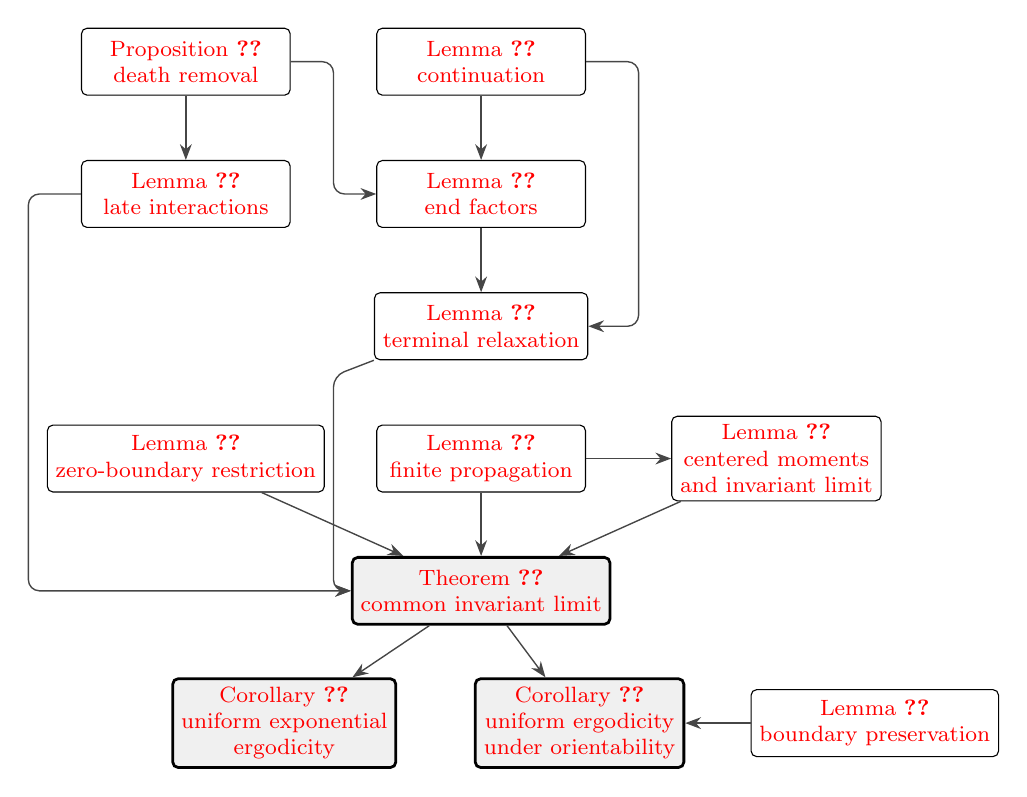
\begin{tikzpicture}[
  x=1.25cm,y=1.05cm,
  res/.style={draw,text=red,rounded corners=2pt,align=center,font=\footnotesize,
    minimum width=2.65cm,minimum height=0.85cm,inner sep=3pt,fill=white},
  main/.style={res,line width=1pt,fill=gray!12},
  dep/.style={-{Stealth[length=2mm]},line width=0.5pt,gray!55!black,rounded corners=4pt}
]
\node[res] (death) at (-2,0) {Proposition~\ref{prop:death-removal}\\death removal};
\node[res] (continue) at (1,0) {Lemma~\ref{prop:no-late-continuation-identity}\\continuation};
\node[res] (late) at (-2,-1.6) {Lemma~\ref{lem:late-interactions}\\late interactions};
\node[res] (end) at (1,-1.6) {Lemma~\ref{lem:end-factor-relaxation}\\end factors};
\node[res] (relax) at (1,-3.2) {Lemma~\ref{lem:no-late-relaxation}\\terminal relaxation};
\node[res] (compat) at (-2,-4.8) {Lemma~\ref{lem:zero-boundary-compatibility}\\zero-boundary restriction};
\node[res] (propagation) at (1,-4.8) {Lemma~\ref{lem:finite-propagation}\\finite propagation};
\node[res] (cone) at (4,-4.8) {Lemma~\ref{lem:centered-cone-preservation}\\centered moments\\and invariant limit};
\node[main] (main) at (1,-6.4) {Theorem~\ref{thm:common-invariant-limit}\\common invariant limit};
\node[main] (uniform) at (-1,-8) {Corollary~\ref{cor:uniform-exponential-ergodicity}\\uniform exponential\\ergodicity};
\node[main] (oriented) at (2,-8) {Corollary~\ref{cor:oriented-ergodicity}\\uniform ergodicity\\under orientability};
\node[res] (boundary) at (5,-8) {Lemma~\ref{lem:boundary-moment-preservation}\\boundary preservation};
\draw[dep] (death)--(late);
\draw[dep] (death.east)--(-0.5,0)--(-0.5,-1.6)--(end.west);
\draw[dep] (continue)--(end);
\draw[dep] (continue.east)--(2.6,0)--(2.6,-3.2)--(relax.east);
\draw[dep] (end)--(relax);
\draw[dep] (late.west)--(-3.6,-1.6)--(-3.6,-6.4)--(main.west);
\draw[dep] (relax.south west)--(-0.5,-3.8)--(-0.5,-6.4)--(main.west);
\draw[dep] (compat)--(main);
\draw[dep] (propagation)--(main);
\draw[dep] (propagation)--(cone);
\draw[dep] (cone)--(main);
\draw[dep] (main)--(uniform);
\draw[dep] (main)--(oriented);
\draw[dep] (boundary)--(oriented);
\end{tikzpicture}}
\caption{\rev{The two estimates and the auxiliary facts used in the
short proof of the main theorem. The separate finite-volume proposition is
a consequence of the same two estimates.}}
\label{fig:dependency-graph}
\end{figure}

\begin{figure}[htbp]
\centering
\resizebox{\linewidth}{!}{%
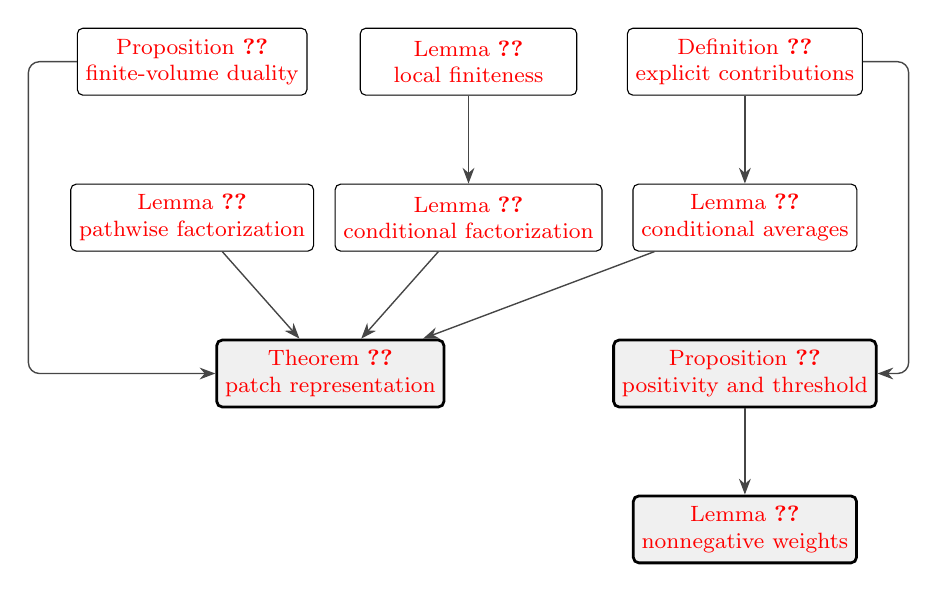
\begin{tikzpicture}[
  x=1.3cm,y=1.1cm,
  res/.style={draw,text=red,rounded corners=2pt,align=center,font=\footnotesize,
    minimum width=2.75cm,minimum height=0.85cm,inner sep=3pt,fill=white},
  main/.style={res,line width=1pt,fill=gray!12},
  dep/.style={-{Stealth[length=2mm]},line width=0.5pt,gray!55!black,rounded corners=4pt}
]
\node[res] (dual) at (-2.7,0) {Proposition~\ref{thm:monomial-duality}\\finite-volume duality};
\node[res] (local) at (0,0) {Lemma~\ref{lem:dual-local-finiteness}\\local finiteness};
\node[res] (formulas) at (2.7,0) {Definition~\ref{def:patch-contributions}\\explicit contributions};
\node[res] (path) at (-2.7,-1.8) {Lemma~\ref{lem:pathwise-factorization}\\pathwise factorization};
\node[res] (factor) at (0,-1.8) {Lemma~\ref{thm:patch-factorization}\\conditional factorization};
\node[res] (averages) at (2.7,-1.8) {Lemma~\ref{lem:contribution-formulas}\\conditional averages};
\node[main] (rep) at (-1.35,-3.6) {Theorem~\ref{thm:patch-representation}\\patch representation};
\node[main] (positive) at (2.7,-3.6) {Proposition~\ref{prop:patch-contribution-positivity}\\positivity and threshold};
\node[main] (weight) at (2.7,-5.4) {Lemma~\ref{lem:nonnegative-patch-weights}\\nonnegative weights};
\draw[dep] (dual.west)--(-4.3,0)--(-4.3,-3.6)--(rep.west);
\draw[dep] (local)--(factor);
\draw[dep] (path)--(rep);
\draw[dep] (factor)--(rep);
\draw[dep] (formulas)--(averages);
\draw[dep] (averages)--(rep);
\draw[dep] (formulas.east)--(4.3,0)--(4.3,-3.6)--(positive.east);
\draw[dep] (positive)--(weight);
\end{tikzpicture}}
\caption{\rev{The construction and interpretation of the patch representation.
Definitions of the skeleton, patch laws, consistency events and patch weights
precede the results that use them.}}
\label{fig:dependency-graph-sec4}
\end{figure}
\FloatBarrier

\begin{table}[htbp]
\centering
\footnotesize
{\color{red}
\begin{tabularx}{\linewidth}{@{}lX@{}}
\hline
\rev{Result} & \rev{Its proof uses}\\
\hline
Theorem~\ref{thm:patch-representation} &
Proposition~\ref{thm:monomial-duality};
Lemmas~\ref{thm:patch-factorization}, \ref{lem:pathwise-factorization},
\ref{lem:contribution-formulas}\\
Proposition~\ref{prop:patch-contribution-positivity} &
Definition~\ref{def:patch-contributions} and its spin-rate formulas\\
Lemma~\ref{lem:nonnegative-patch-weights} &
Proposition~\ref{prop:patch-contribution-positivity}\\
Proposition~\ref{prop:death-removal} &
The generator identity, the contribution formulas, and
Proposition~\ref{prop:patch-contribution-positivity}\\
Lemma~\ref{lem:late-interactions} &
Proposition~\ref{prop:death-removal};
Theorem~\ref{thm:patch-representation};
Lemma~\ref{lem:dual-local-finiteness}\\
Lemma~\ref{prop:no-late-continuation-identity} &
Lemmas~\ref{thm:patch-factorization}, \ref{lem:contribution-formulas};
the composition identity for~$\psi_i$\\
Lemma~\ref{lem:end-factor-relaxation} &
Lemma~\ref{prop:no-late-continuation-identity};
Proposition~\ref{prop:death-removal}\\
Lemma~\ref{lem:no-late-relaxation} &
Lemmas~\ref{prop:no-late-continuation-identity}, \ref{lem:end-factor-relaxation},
\ref{lem:late-interactions}\\
Proposition~\ref{prop:finite-volume-convergence} &
Lemmas~\ref{lem:late-interactions}, \ref{lem:no-late-relaxation}\\
Lemma~\ref{lem:centered-cone-preservation} &
Proposition~\ref{prop:patch-contribution-positivity};
Lemma~\ref{lem:finite-propagation}\\
Theorem~\ref{thm:common-invariant-limit} &
Lemmas~\ref{lem:late-interactions}, \ref{lem:no-late-relaxation},
\ref{lem:finite-propagation}, \ref{lem:zero-boundary-compatibility},
\ref{lem:centered-cone-preservation}\\
Corollary~\ref{cor:oriented-ergodicity} &
Theorem~\ref{thm:common-invariant-limit};
Lemma~\ref{lem:boundary-moment-preservation}\\
Corollary~\ref{cor:infinite-volume-representation} &
Theorem~\ref{thm:patch-representation};
Lemmas~\ref{lem:nonnegative-patch-weights}, \ref{lem:finite-propagation},
\ref{lem:dual-local-finiteness}\\
Lemma~\ref{lem:spatial-confinement} &
Lemma~\ref{prop:confined-interaction-identity};
Corollary~\ref{cor:infinite-volume-representation}\\
Corollary~\ref{cor:invariant-patch-moments} &
Theorem~\ref{thm:common-invariant-limit};
Corollary~\ref{cor:infinite-volume-representation};
the late-interaction and confined relaxation bounds;
Lemma~\ref{lem:spatial-confinement}\\
\hline
\end{tabularx}
}
\caption{\rev{Dependencies in the revised proof order. The last three results
belong to Appendix~\ref{app:spatial-confinement}.}}
\label{tab:dependencies}
\end{table}
\FloatBarrier

\bibliographystyle{amsplain-fullnames}
\bibliography{references}

\end{document}
